\chapter{Application: Cardiac Mechanics}
\label{chap:5}
%
Provided the image-based meshing workflow that has been fully developed in~\chapref{3}, together with the finite element approaches established in~\chapref{4}, the entire image-based modeling and simulation pipeline can now be demonstrated. The application of choice is the mechanical behavior of a beating human heart. Cardiac mechanics is a good testbed for the particular image-based modeling and simulation workflow described because: 1) the application only involves binary image masks, 2) the exact geometry does not grossly affect results since contact modeling is not included, and 3) the use of simulation in this field arguably has the potential to save and improve more lives than any other biomechanics application area.

This chapter introduces and motivates the task of modeling the human heart. The essential components to computational cardiac mechanics are described for an implementation using conventional finite elements, and simulation results are presented. Finally, the details of implementing the same mechanics into a polyhedral finite element code are discussed, together with a suite of verification tests and results.

\section{Introduction}

A brief overview of the anatomy and function of the heart will be presented, followed by a survey of approaches found in the literature.

\subsection{Anatomy and Function of the Heart}
The heart consists of four chambers: the \textit{left ventricle} (LV), \textit{right ventricle} (RV), \textit{left atrium} (LA), and \textit{right atrium} (RA) (See~\figref{anatomy}). The \textit{septum} is the tissue wall that separates the LV and RV. The thinner-walled atria act as blood reservoirs for the ventricles, which are predominantly responsible for the pumping function. The entire heart is encompassed by a fibrous sac known as the \textit{pericardium}, which resists rapid increases in cardiac size. The primary function of the heart is to pump blood throughout the body, delivering nutrients and removing waste from each organ~\cite{holzapfel_2009}. Cyclic pumping of the heart arises from the interaction of its electrical and mechanical function. Namely, the electrical activation of cardiac muscle fibers causes an excitation and contraction of tissue that drives the motion of the organ. Myocardial tissue consists of discrete muscle fiber bundles that exhibit orthotropic material behavior. For a more detailed description of the macro- and microstructural properties of the heart, refer to Holzapfel \textit{et al.}~\cite{holzapfel_2009} and Hunter~\cite{holzapfel_2009} 

\begin{figure}[htbp!]
\centering
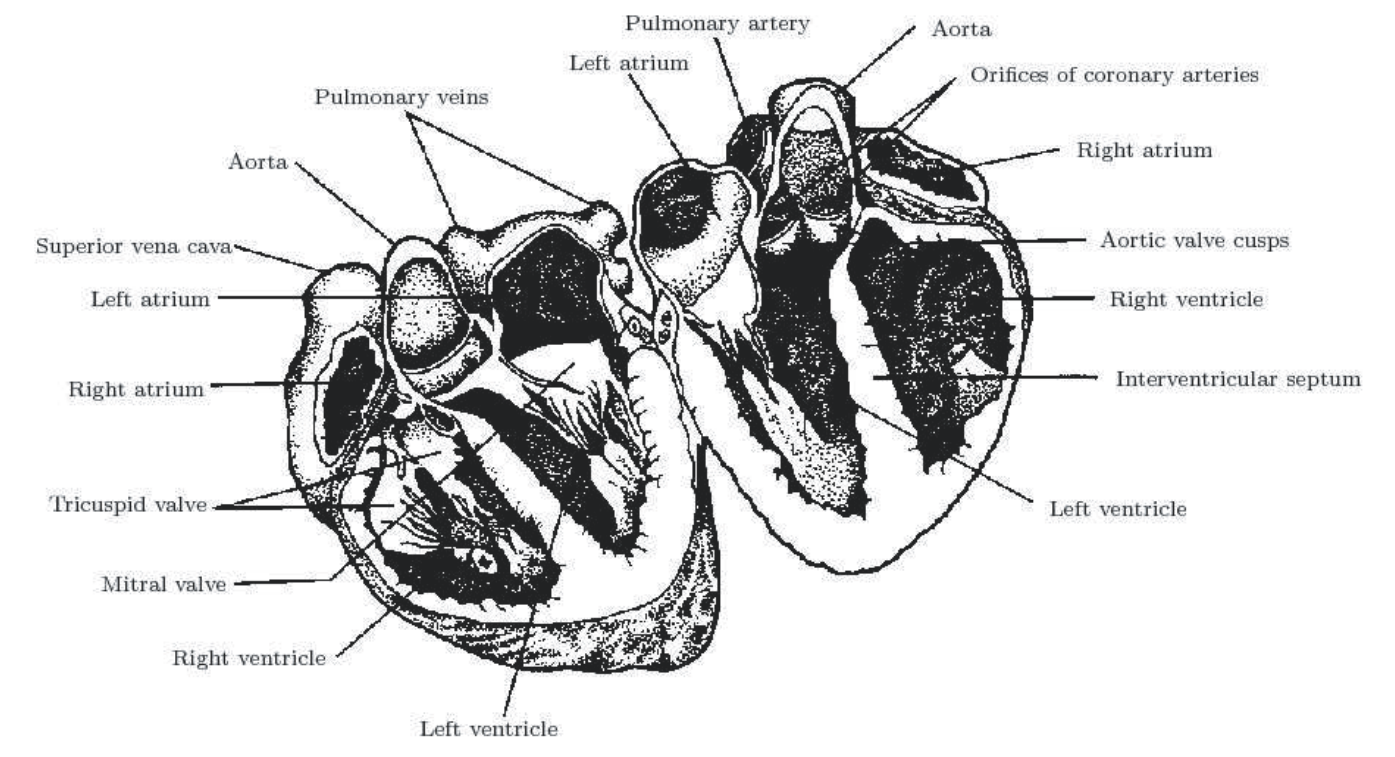
\includegraphics[width=1.0\textwidth]{media/anatomy.png}
\caption{Longitudinal cross-section of the human heart~\cite{katz_2015}}
\label{fig:anatomy}
\end{figure}

\subsection{Related Work}
Cardiovascular disease is the leading cause of death and disability, accounting for about 40$\%$ of all human mortality~\cite{genet_2015}. Heart failure is one of the most common, costly, and deadly medical conditions, affecting more than 25 million people worldwide~\cite{mann_2015}. Better understanding the nuanced electrical and mechanical behavior of normal and pathological hearts is an important step in improving treatment for heart disease. The complexity of the mechanisms of interest, time and cost savings offered by simulation, and the high sensitivity to various patient-specific parameters make \textit{in silico} modeling an important tool in addressing the problem.

Indeed, cardiac mechanics is one of the most mature fields in computational biomechanics. Several well-known groups have advanced the field using a variety of approaches with respect to the geometry and meshing. \textit{The Living Heart Project}~\cite{genet_2015, baillargeon_2014} has arguably gained the most traction in advancing the understanding of whole-heart cardiac mechanics through simulation, albeit using linear tetrahedra for an artificial heart geometry that was not generated from medical imaging. Augustin \textit{et al.}~\cite{augustin_2016} also used linear tetrahedral finite elements, meshed from considerably smoothed surfaces originating from MRI data. Several research groups still only model simplified geometries of the left ventricle~\cite{guccione_2005, sack_2016}, in conjunction even with cubic Hermite finite elements~\cite{mcculloch_2000}. Generally speaking, though, most modern approaches generate either bi-ventricular models (i.e., left and right ventricles) or whole heart models that include the atria and potentially other geometric structures.

Gurev \textit{et al.}~\cite{gurev_2015} performed mechanical simulations on a quadratic hex-dominant mixed element mesh of the human heart ventricles, whose work forms the basis for the cardiac mechanics simulations detailed in this chapter. The review article by Trayanova \textit{et al.}~\cite{trayanova_2011} provides an excellent summary of the various components involved in ventricular electromechanical modeling, many of which are discussed here.

\section[Demonstration using Conventional Finite Elements]{Demonstration using Conventional Finite \\ Elements}

\textit{Cardioid} is a highly efficient and scalable code at Lawrence Livermore National Laboratory that utilizes high performance computing for modeling the electromechanics of cardiac arrhythmia~\cite{richards_2013, gurev_2015}. The key features of the code will be highlighted, as is relevant to image-based cardiac mechanics modeling, and as a demonstration tool for image-based modeling and simulation pipeline using conventional finite element methods.

%%%%%%%%%%%%%%%%%%%%%%%%%%%%%%%%%%%%%%%%%%%%%%%
%%%%%%%%%%%%%%%%%%%%%%%%%%%%%%%%%%%%%%%%%%%%%%%
\subsection{Methods}
\label{Methods}

In Cardioid, the heart is assumed to undergo quasi-static finite deformations, gravitational body forces are assumed negligible, and the stress measure of interest is the second Piola-Kirchoff stress $\bm{S}$. Thus, balance of linear momentum reduces to the following equation:
\begin{equation}
(F_{ik}S_{kj}),_{j} = 0
\end{equation}

In order to fully define and solve these equations, the following are specified: the mesh, constitutive update, solution-dependent pressure boundary conditions, and the finite element solver. Each consideration will be described in turn.

%%%%%%%%%%%%%%%%%%%%%%%%%%%%%%%%%%%%%%%%%%%%%%%
%%%%%%%%%%%%%%%%%%%%%%%%%%%%%%%%%%%%%%%%%%%%%%%
\subsubsection{Mesh Generation}
\label{Mesh Generation}

A bi-ventricular mesh is generated using the procedures described in~\chapref{2} and \chapref{3}. Namely, an MRI of an \textit{ex vivo} human heart from the CardioVascular Research~\cite{cvgg} is segmented using the software Seg3D. Since the ventricles are most responsible for the pumping action, image segmentation is restricted to those geometric structures. A threshold segmentation is applied, and then used as the initial seed to Seg3D's level set segmentation tool. Additional tools to fill holes and dilate-erode the image mask are utilized before a final sweep of manual paintbrushing is employed. Following careful manual inspection, the final image mask is input to Shabaka to generate a high quality surface of the heart ventricles with a total of 50k points. Tetgen is invoked to produce a tetrahedral mesh that honors the input surface and attempts to produce high quality tetrahedra for the purposes of finite element simulations. A maximum element volume of 2 \textit{mm$^3$} was imposed. Again, quadratic tetrahedral elements are chosen in favor of linear elements to avoid volumetric locking and/or impracticably fine meshes. The surface and volume meshes are shown in \figref{tetmesh} - the final quadratc tetrahedral mesh has 374k elements and 595k nodes.

%%%%%%%%%%%%%%%%%%%%%%%%%%%%%%%%%%%%%%%%%%%%%%%
%%%%%%%%%%%%%%%%%%%%%%%%%%%%%%%%%%%%%%%%%%%%%%%
\subsubsection{Material Model}
\label{Material Model}

The cardiac tissue is assumed to exhibit an additive stress decomposition, such that $\bm{S} = \bm{S}_p + \bm{S}_a$ at any point in the model. The \textit{active stress} $\bm{S}_a$ represents the stress induced through active contraction of muscle fibers, and the \textit{passive stress} $\bm{S}_p$ is the stress experienced by the surrounding tissue.

\textbf{Passive Stress}

The passive response of the cardiac tissue is characterized by an incompressible, transversely isotropic constitutive law by Usyk~\textit{et al.}~\cite{usyk_2002}. The strain energy density functional is given by:
\begin{gather}
W(\bm{C}) = \frac{C}{2}\left(e^Q -1\right) \\
Q = b_{ff} E^2_{ff} + b_{ss} E^2_{ss} + b_{nn} E^2_{nn} + b_{fs}\left(E^2_{fs} + E^2_{sf}\right) + b_{fn}\left(E^2_{fn} + E^2_{nf}\right) + b_{ns}\left(E^2_{ns} + E^2_{sn}\right)
\label{eqn:usyk}
\end{gather}
where $\bm{E} = \frac{1}{2}(\bm{C} - \bm{I})$ is the Green-Lagrange strain tensor expressed in a local orthonormal coordinate system with axes parallel to the local fiber, sheet, and sheet-normal $(f,s,n)$ directions, and $C$, $b_{ff}$, $b_{ss}$, $b_{nn}$, $b_{fs}$, $b_{fn}$, and $b_{ns}$ are material parameters.

Incompressibility is fully enforced by solving for pressure unknowns as Lagrange multipliers in addition to nodal unknowns. In order to use the constitutive law in a fully incompressible context, the deviatoric and volumetric portions of the strain energy are separated as is done by Weiss~\textit{et al.}~\cite{weiss_1996}. Rather than defining the passive stress as simply $\bm{S}_p = \frac{\partial W}{\partial \bm{E}}$, the passive stress becomes:
\begin{equation}
\bm{S}_p= 2\frac{\partial{\tilde{W}(\tilde{\bm{C}})}}{\partial{\bm{C}}} - pJ\bm{C}^{-1}
\end{equation}
where $\tilde{W}(\tilde{\bm{C}})$ is the deviatoric component of the strain energy functional, $J = \text{det}(\bm{F})$, and $\tilde{\bm{C}} = J^{-2/3}\bm{C}$. More details regarding the enforcement of incompressibility can be found in Gurev \textit{et al.}~\cite{gurev_2015} and Weiss~\textit{et al.}~\cite{weiss_1996}.

\textbf{Active Stress}

The active stress is defined as :
\begin{equation}
\bm{S}_a = \sigma_a \bm{f} \bm{f}^{T}
\label{eqn:active}
\end{equation}
where $\bm{f}$ is the muscle fiber direction and ${\sigma_a}$ is the scalar active tension induced in the fiber direction. The vector $\bm{f}$ here may refer to the fiber orientation either in the reference configuration or the current configuration - within Cardioid it refers to the direction in the reference configuration.

The model by Lumens \textit{et al.}~\cite{lumens_2009} is used to determine the active tension $\sigma_a$ in the following manner:
\begin{align}
\frac{d\bm{w}}{dt} = \bm{q}(\bm{w}; t_a, \lambda) \\
\sigma_a \equiv \sigma_a(\bm{w}; t_a, \lambda)
\end{align}
The scalar active tension depends on the state variables $\bm{w}$ of the muscle cells, the time $t_a$ at which the muscle cells electrically activate, and the muscle fiber stretch $\lambda$ in the direction of $\bm{f}$. Specifically, the fiber stretch is defined as $\lambda = (\bm{f}\bm{C}\bm{f}^T)^{1/2}$. The state variables are updated using a forward Euler scheme within the constitutive update. Further details on the state variables $\bm{w}$ and the way in which they are updated via $\bm{q}$ can be found in the work by Lumens~\textit{et al.}~\cite{lumens_2009}.

The activation time $t_a$ at each integration point is gathered from the results of the electrophysiology portion of the Cardioid code~\cite{richards_2013}. Specifically, an electrostatics problem is solved numerically for time-varying voltages, and the activation time is determined based on when the voltage at each location passes a certain threshold. A one-way coupling is thus imposed, in which the mechanics code depends on the electrophysiology results, but not vice versa. A fixed beat duration $t_b$ is assumed, such that the myofilament model excites and contracts for the $n$th beat at time $(n-1)t_b + t_a$. Activation times are stored in the mechanics code as a field variable within the bi-ventricular mesh (see \figref{supp1}).

\begin{sidewaysfigure}[htbp!]
\centering
\subfigure[]{%
		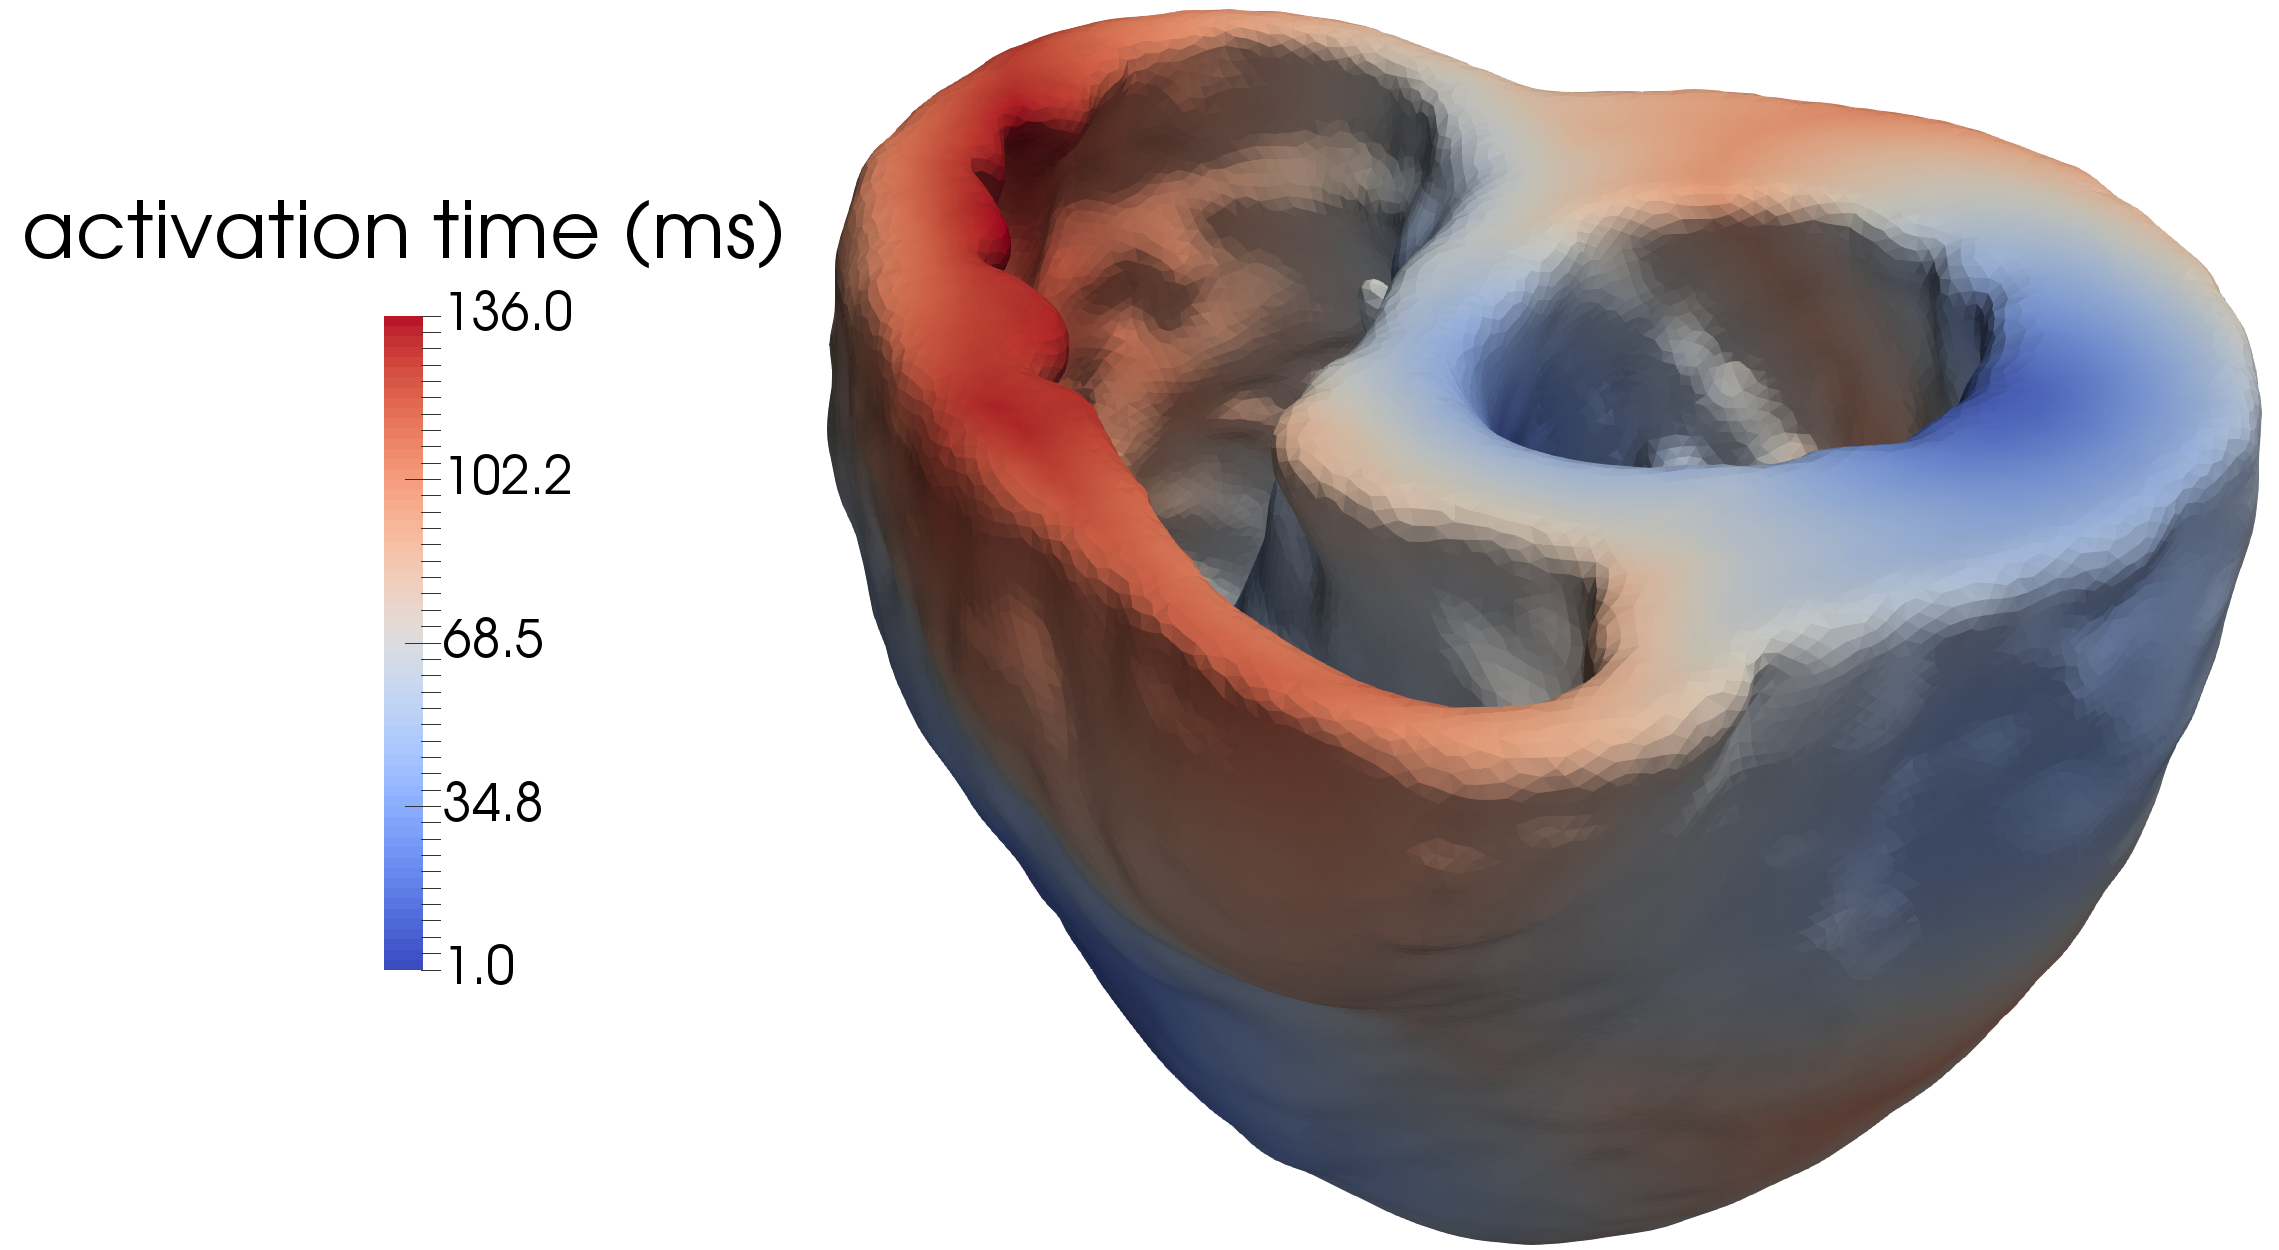
\includegraphics[scale=0.11]{media/4-cardioid/22-activationtime.png}
\label{fig:supp1}}
\subfigure[]{%
		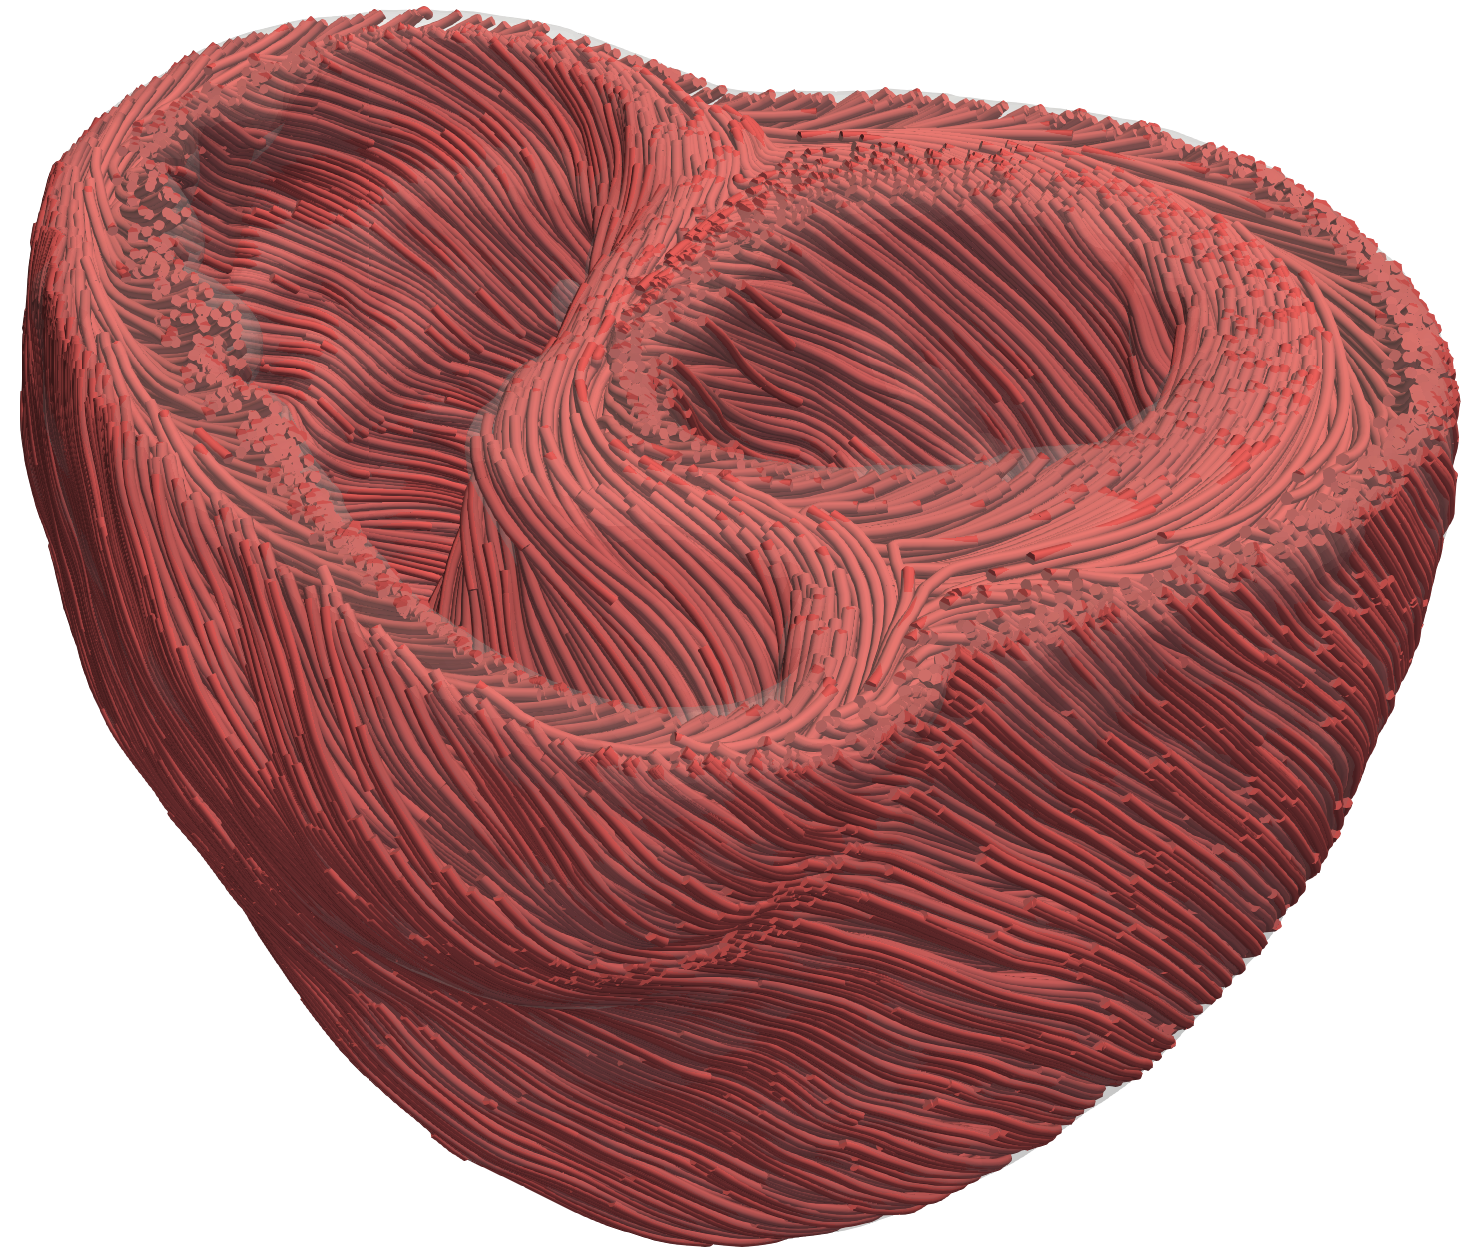
\includegraphics[scale=0.11]{media/4-cardioid/3-fibers.png}
\label{fig:supp2}}
\subfigure[]{%
		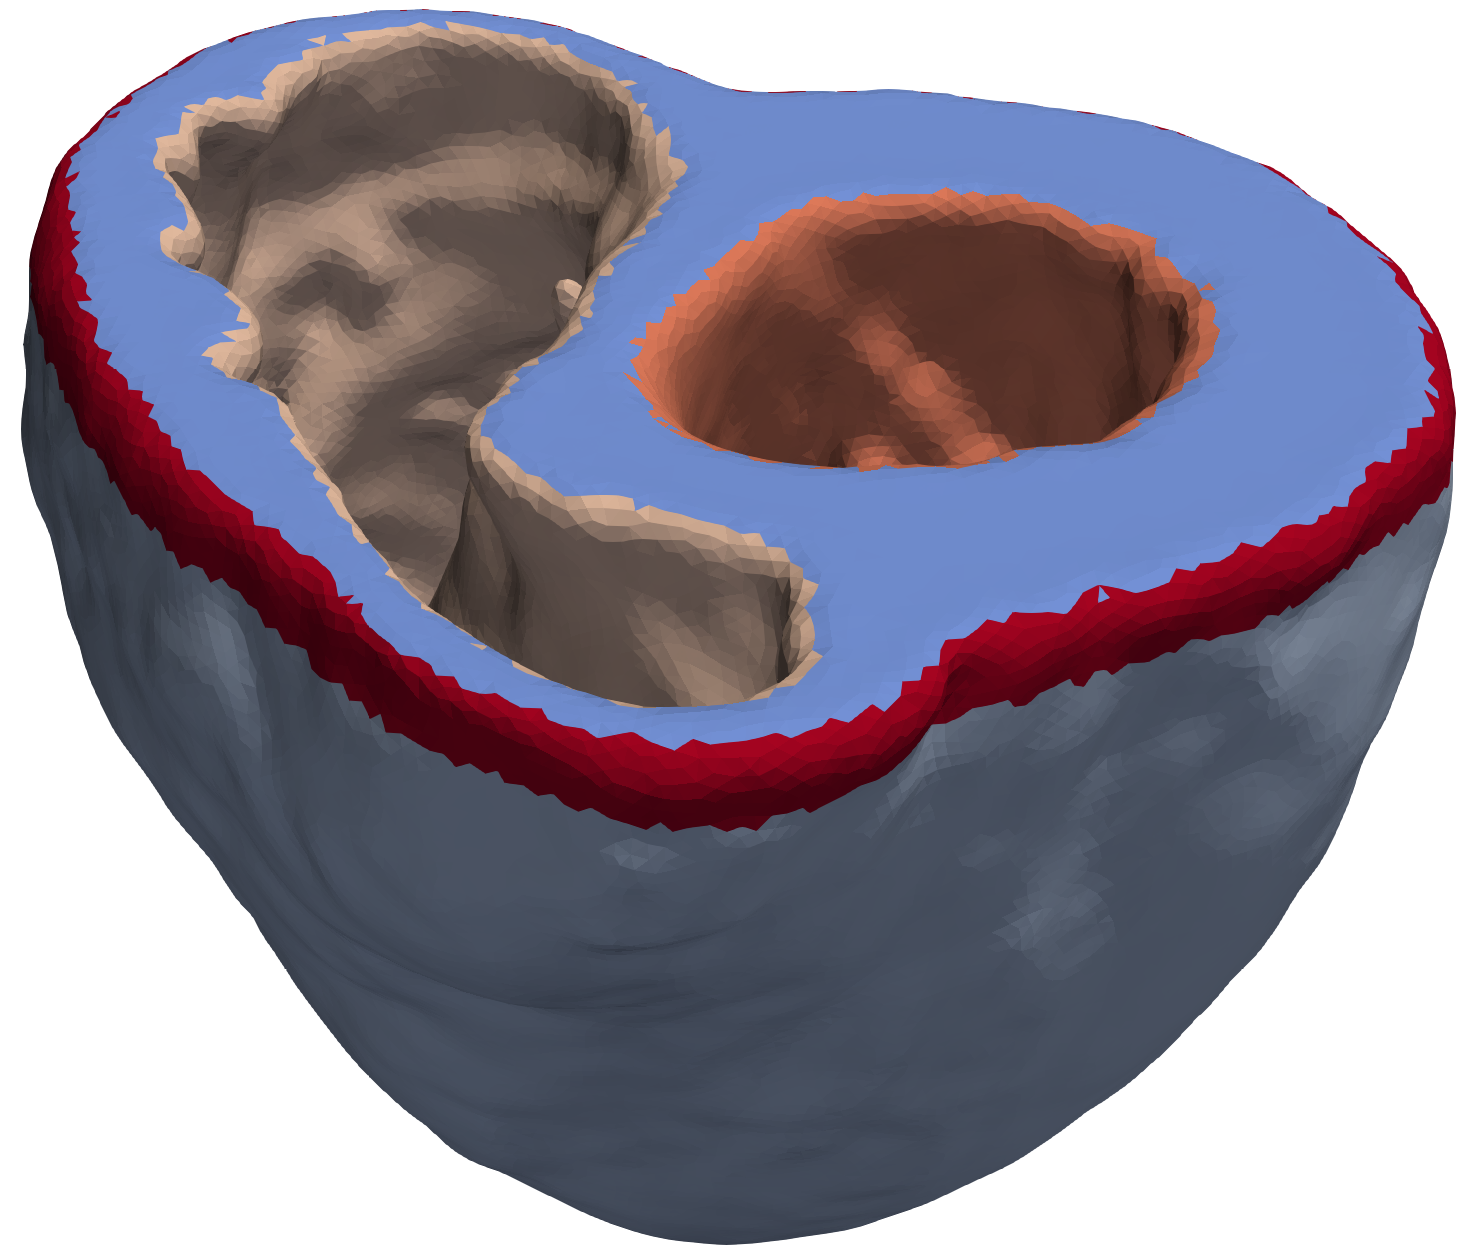
\includegraphics[scale=0.11]{media/4-cardioid/4-tagged.png}
\label{fig:supp3}}
%
\caption{Mechanics modeling considerations: (a) electrical activation times, (b) muscle fiber orientations, and c) surface tagging and prescription of corresponding boundary conditions.}
\label{fig:supp}
\end{sidewaysfigure}

\textbf{Fiber Generation}

Both the passive and active portions of the constitutive model depend on the muscle fiber orientation. Fiber orientations may be generated directly from DTMRI data, but that process requires denoising, smoothing, and interpolating tensor datasets, which can lead to unsatisfactory results. Additionally, DTMRI data is more expensive to acquire, and may not always be available. The Cardioid fiber generation code opts for the more popular \textit{rule-based approach}, in which fiber orientations are artificially generated based on the input mesh. The code utilizes the algorithm by Bayer \textit{et al.}~\cite{bayer_2012}, which involves solving Laplace's equation $\nabla^2\phi = 0$ four times, each with different Dirichlet boundary conditions (see~\figref{bayer}).

\begin{figure}[ht]
\centering
		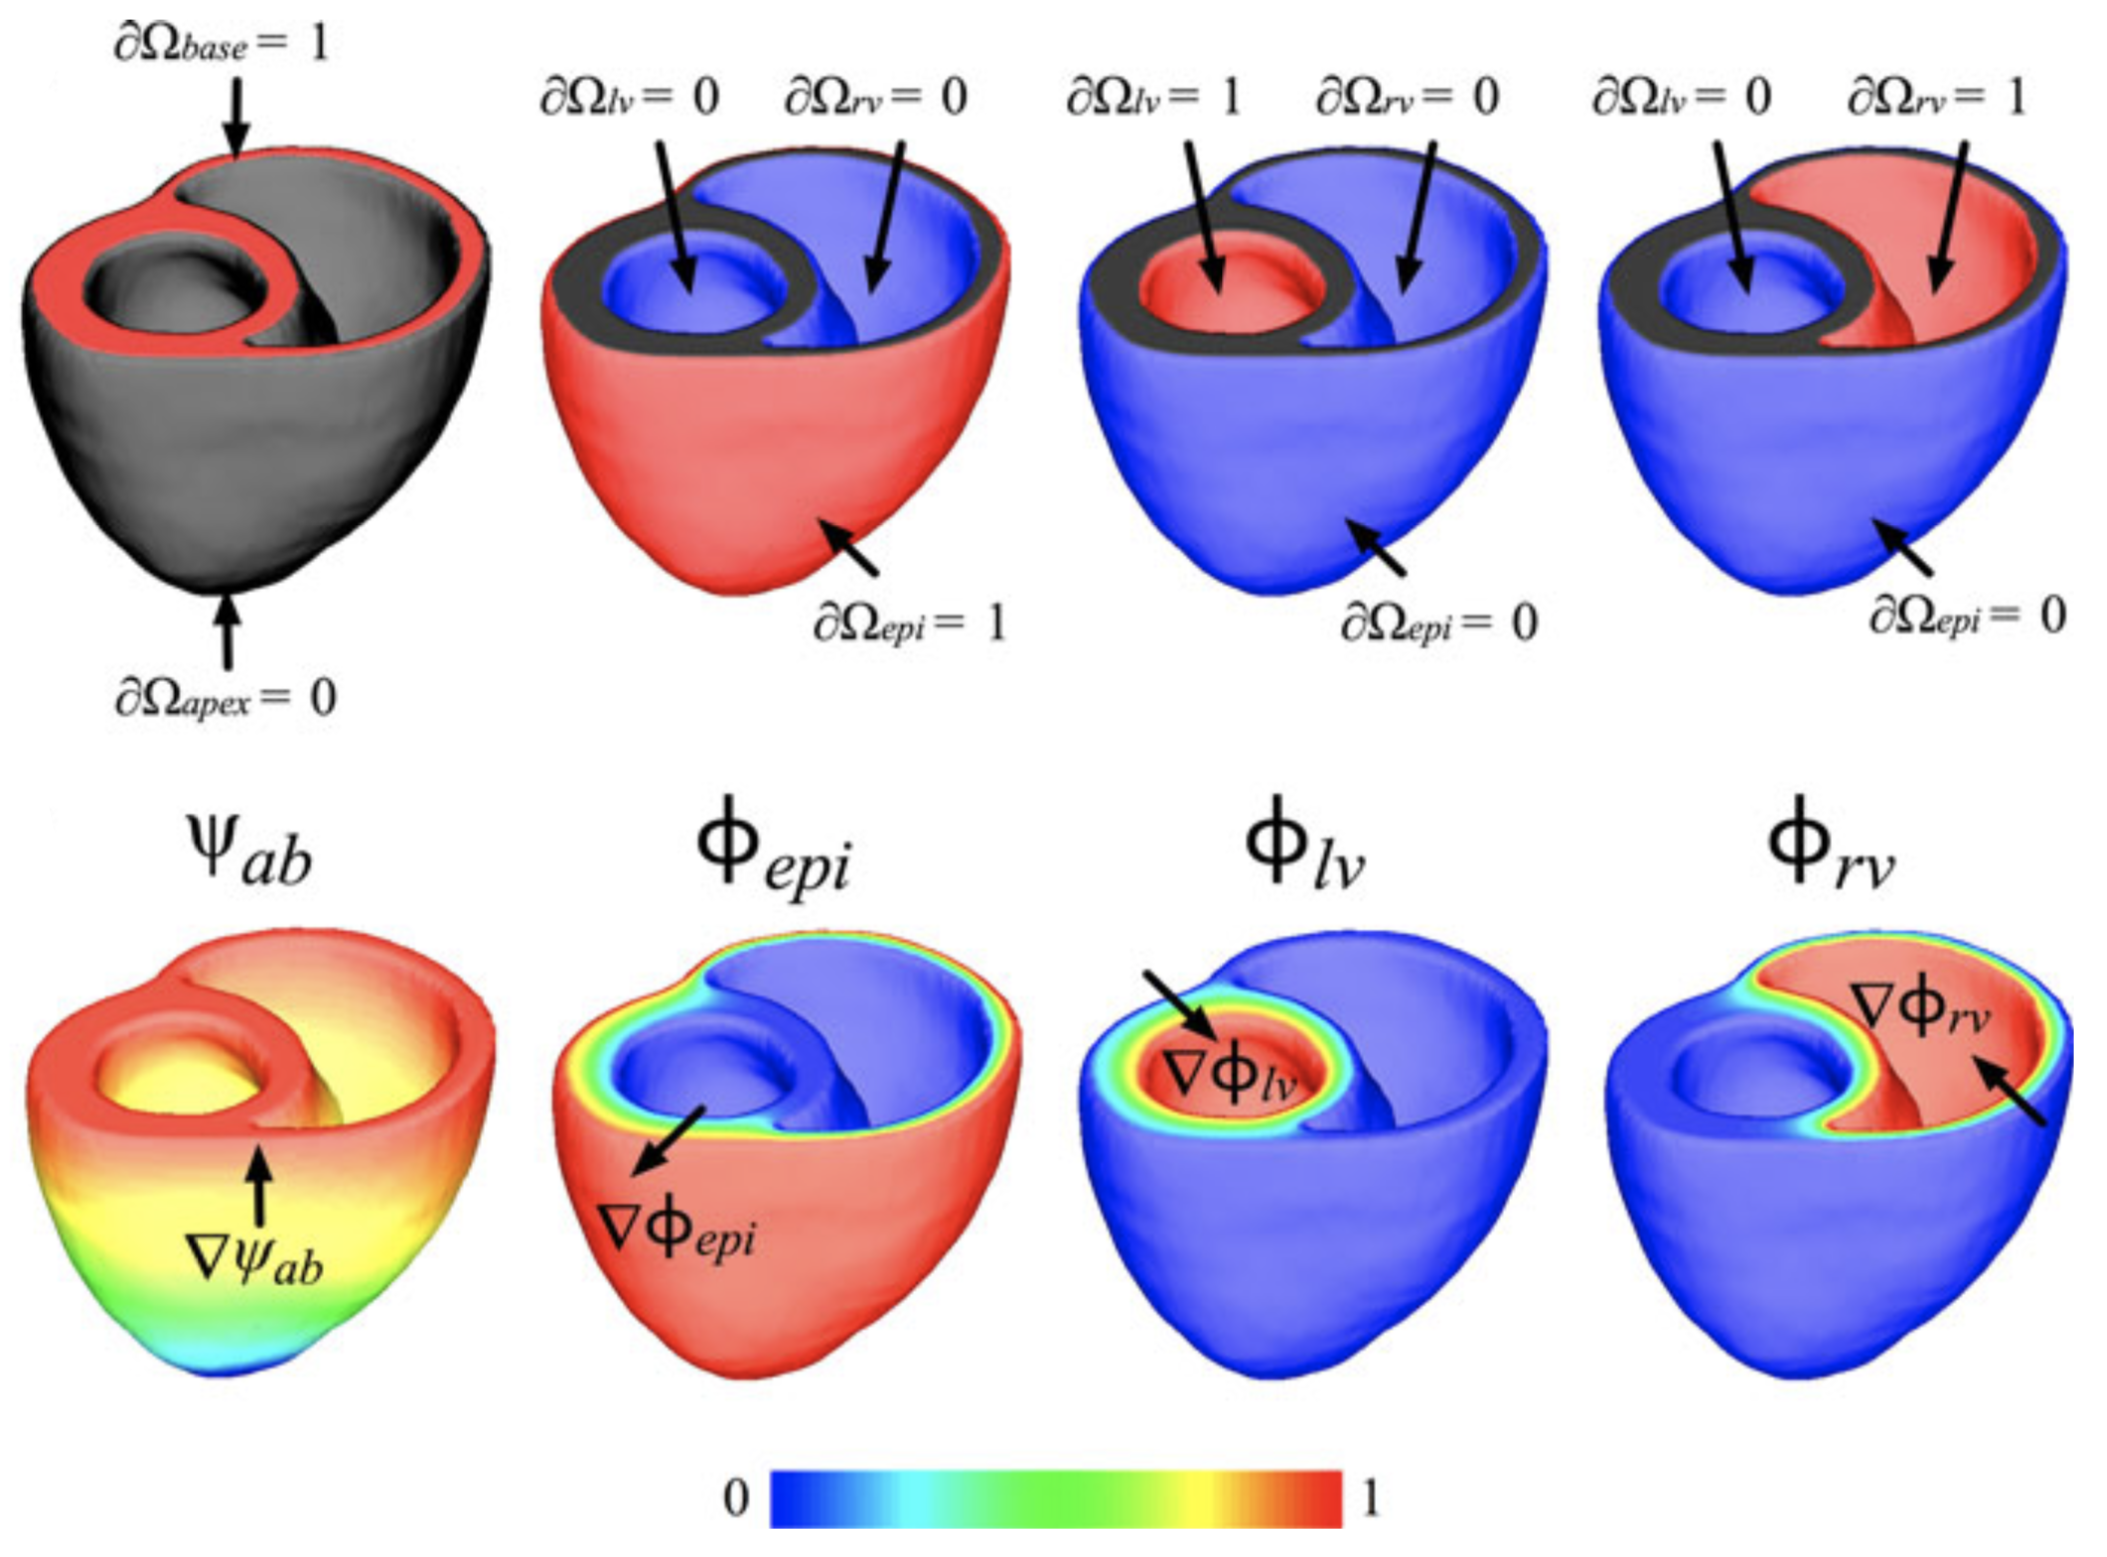
\includegraphics[scale=0.3]{media/bayer.png}
\caption{Boundary conditions and resulting scalar solutions to Laplace's equation in Bayer \textit{et al.}~\cite{bayer_2012}. The gradients of the solutions are used to construct the rule-based fiber orientations}
\label{fig:bayer}
\end{figure}

The gradients of these solutions inform the construction of orthotropic fiber orientations at each solution point. Fiber orientations are then interpolated at the junctions between the LV, RV, and septum to ensure that the fiber direction changes smoothly and continuously throughout the entire myocardium. The details by which the gradients are used to construct the fiber orientations and by which orientations are interpolated are explained in Bayer~\textit{et al.}~\cite{bayer_2012}. The Laplace solves are performed using the highly parallelized finite element code \textit{MFEM}~\cite{mfem-library} on the same input quadratic tetrahedral mesh to be used for the mechanics simulation. The algorithm performs robustly for various geometries and compares well with fiber orientations generated directly from DTMRI data. The computed fiber orientations for the mesh of interest are shown in \figref{supp2}.

%%%%%%%%%%%%%%%%%%%%%%%%%%%%%%%%%%%%%%%%%%%%%%%
%%%%%%%%%%%%%%%%%%%%%%%%%%%%%%%%%%%%%%%%%%%%%%%
\subsubsection{Boundary Conditions}
\label{Boundary Conditions}

Fluid flow and fluid-structure interaction are not yet implemented in the Cardioid code, so ventricular volume constraints are imposed to mimic the effect of blood flow. The volumes of the ventricle cavities are calculated based on a lumped circulatory model by Kerckhoffs \textit{et al.}~\cite{kerckhoffs_2006}, which are in turn used to determine the time-varying, solution-dependent pressure boundary conditions.

A system of coupled ODEs describing the time evolution of the left ventricle volume $V_{LV}$ and the right ventricle volume $V_{RV}$ for the circulatory model can be written in the form:
\begin{align}
\frac{d\bm{w}_{c}}{dt} = \bm{q}_c(\bm{w}_c, p_{LV}, p_{RV}; t) \\
\frac{dV_{LV}}{dt} = g_{LV}(p_{LV}, \bm{w}_c; t) \\
\frac{dV_{RV}}{dt} = g_{RV}(p_{RV}, \bm{w}_c; t)
\end{align}
where $\bm{w}_c$ is the vector of state variables for the circulatory model, $p_{LV}$ and $p_{RV}$ are the pressures inside the left and right ventricles, and $\frac{dV_{LV}}{dt}$ and $\frac{dV_{RV}}{dt}$ represent the change in blood volume in each of the ventricles. The right hand side functions $\bm{q}_c$, $g_{LV}$, and $g_{RV}$ are described in detail in Kerckhoffs~\textit{et al.}~\cite{kerckhoffs_2006}. This paradigm assumes both that the blood is an incompressible fluid, and that the pressure is spatially uniform within each ventricle. For each time step, the ventricular volumes are calculated from the circulatory model and imposed as constraints on the finite element mesh to determine the corresponding ventricular pressures. The details by which the pressures are computed from the volume constraint are detailed in Gurev~\textit{et al.}~\cite{gurev_2015}. The lumped circulatory model is shown in~\figref{bcs}.
\begin{figure}[ht]
\centering
		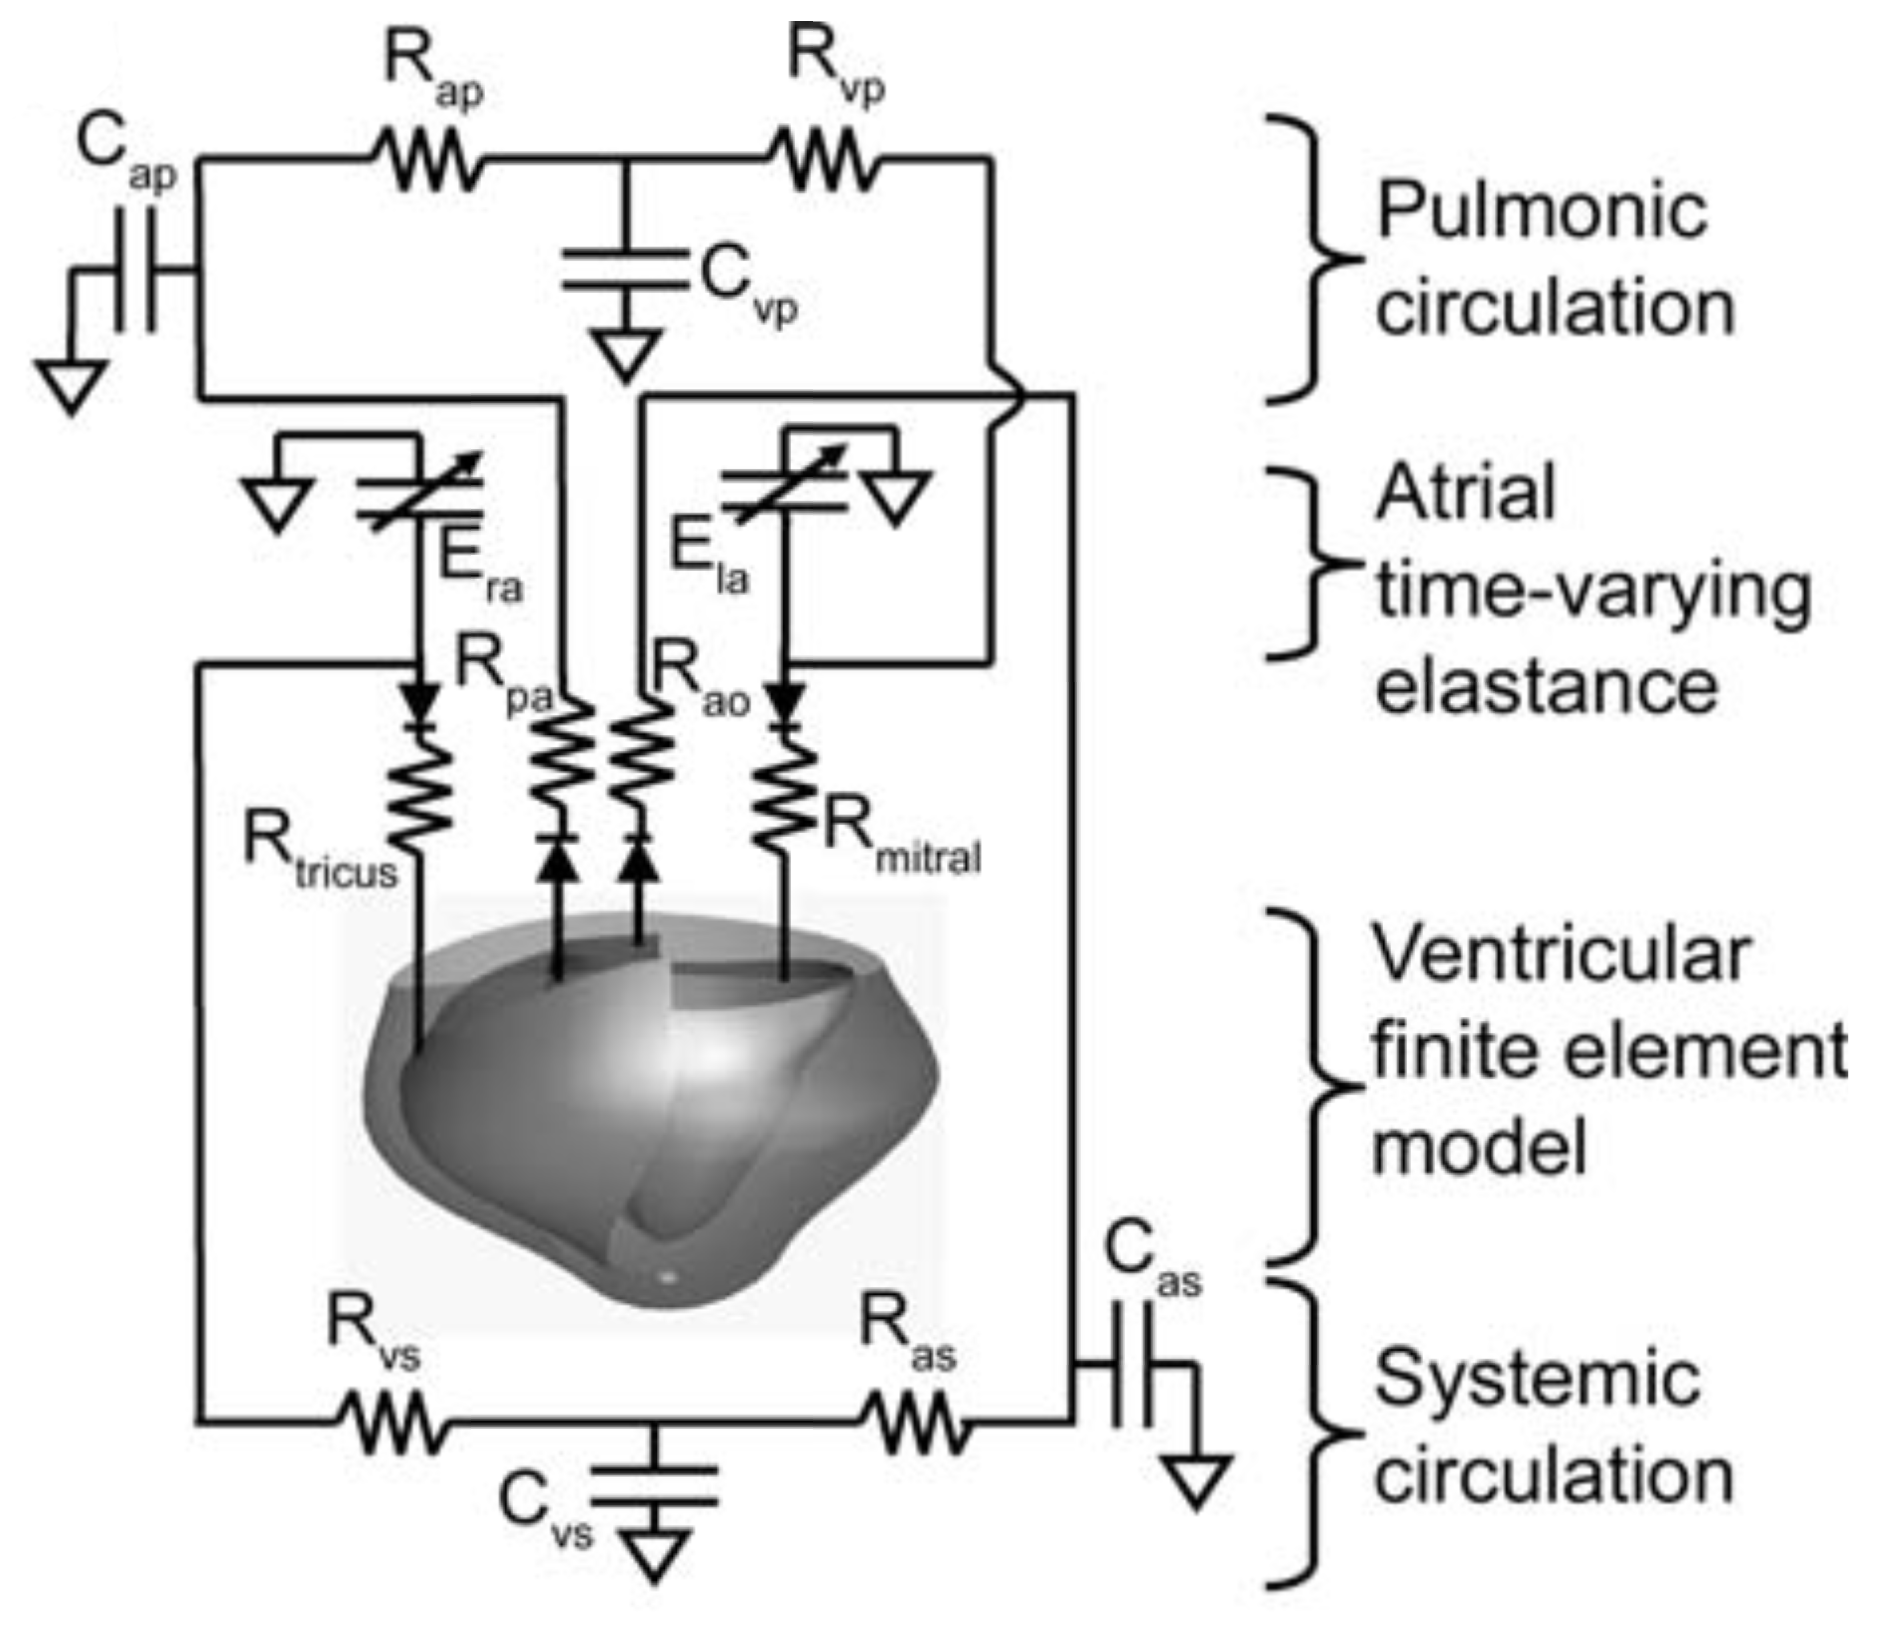
\includegraphics[scale=0.3]{media/bcs.png}
\caption{Lumped circulatory model of Kerckhoffs \textit{et al.}~\cite{kerckhoffs_2006}. Variables shown in the schematic are parameters in the coupled system of ODEs, which are solved to obtain ventricular volumes at each time step.}
\label{fig:bcs}
\end{figure}

In order to avoid highly nonlinear solutions at the start of the simulation, initial pressures are applied linearly in the first 100 ms prior to ``turning on'' the active contraction and ventricular boundary conditions. The first 100 ms may be viewed as the period in which a residual stress is applied.

Displacement boundary conditions are enforced such that the base of the heart is not allowed to move out of plane, and that a strip of the epicardium near the base experiences zero displacements in all directions. In order to enforce these displacement and pressure BCs, the appropriate surfaces must be identified. Identification of the base, epicardium, left ventricle, and right ventricle is a necessary intermediate step in generating fiber directions, so those boundary condition tags are available following execution of the fiber generation code (see~\figref{supp3}).

%%%%%%%%%%%%%%%%%%%%%%%%%%%%%%%%%%%%%%%%%%%%%%%
%%%%%%%%%%%%%%%%%%%%%%%%%%%%%%%%%%%%%%%%%%%%%%%
\subsubsection{Solver}
\label{Solver}

The quadratic tetrahedral mesh described previously is used with the material model and boundary conditions to perform conventional finite element simulations in Cardioid. Cardioid employs a modified version of the freely available finite element library \textit{oomph-lib}~\cite{oomph}.

Because Cardioid uses an implicit mechanics approach, a linear system must be solved for each time step for incremental nodal unknowns. In the interest of solving problems with very fine discretizations, Gurev \textit{et al.} avoid direct solvers of the linear system due to their poor scalability. Instead, they employ a Krylov subspace iterative solver, which is more suitable for large scalable problems. The existence of active contraction creates saddle-points in the linear system that are addressed with a novel preconditioner. The details of the iterative solver may be found in Gurev \textit{et al.}~\cite{gurev_2015}.

The simulation was performed on the \textit{Surface} computing platform at Lawrence Livermore National Laboratory. The Moab schedule manager was used to submit the job, which was run on 50 nodes with 16 cores per node, for a total of 800 processes. With an assumed beat duration of 1000 $ms$ for a healthy human heart (i.e., 60 beats per minute), the simulation was run to a time of 5100 ms with a $\Delta t = 1$ $ms$ time increment. The simulation completed roughly one heartbeat per 24 hours of wall clock time. As mentioned, the first 100 ms are used to linearly apply the initial pressures for the simulation. The first beat is discarded to allow the simulation to reach a dynamic steady state, and thus four full beats of a healthy human heart are extracted from the results.

%%%%%%%%%%%%%%%%%%%%%%%%%%%%%%%%%%%%%%%%%%%%%%%
%%%%%%%%%%%%%%%%%%%%%%%%%%%%%%%%%%%%%%%%%%%%%%%
\subsection{Results}
\label{Results}

Simulation results are shown in \figref{pv} and~\figref{snaps}. \figref{pv1} is known as a \textit{P-V loop} of the left ventricle, and \figref{pv2} is a time history plot of the pressures in the left and right ventricles. \figref{pv1} demonstrates the four stages of the cardiac cycle: 1) \textit{isovolumetric contraction} from label a to b, 2) \textit{ventricular ejection} of blood from label b to c, 3) \textit{isovolumetric relaxation} from label c to d, and 4) \textit{ventricular filling} from label d to a~\cite{slideshare}. Isovolumetric contraction and ventricular ejection comprise what is known as \textit{systole}, during which the ventricles are contracting. Isovolumetric relaxation and ventricular filling are known as \textit{diastole}, during which the ventricles are relaxing. The labels in \figref{pv1} correspond to the panels in~\figref{snaps}, which show the fiber stretch $\lambda$ plotted on deformed meshes at different points in the cardiac cycle. During a cycle, fiber stretch ranges from 0.6 to 1.4, certainly justifying the finite deformation approach. The results closely match those in Gurev~\textit{et al.}~\cite{gurev_2015}, in which a different heart geometry and electrophysiology were used. The full video of four heartbeats played at one quarter speed may be viewed at \href{http://youtu.be/RtQKEjdR4MU}{{\url{http://youtu.be/RtQKEjdR4MU}}}.

In the process of performing simulations, the workflow for: generating the mesh, generating fiber orientations, running the electrophysiology code to produce activation times, running the mechanics code, and post-processing results was improved, simplified, and automated via Python scripts. A robust workflow for performing bi-ventricular cardiac mechanics simulations has thus been demonstrated. It will directly facilitate the current Cardioid research project involving machine learning, which requires a robust and timely generation of simulation results for large numbers of patient imaging data. Additional validation of the results, quantitiative metrics for solution quality, and sensitivity studies of the simulation parameters are still necessary before the tools may be used directly for clinical use.

\begin{figure}[ht]
\centering
\subfigure[]{%
		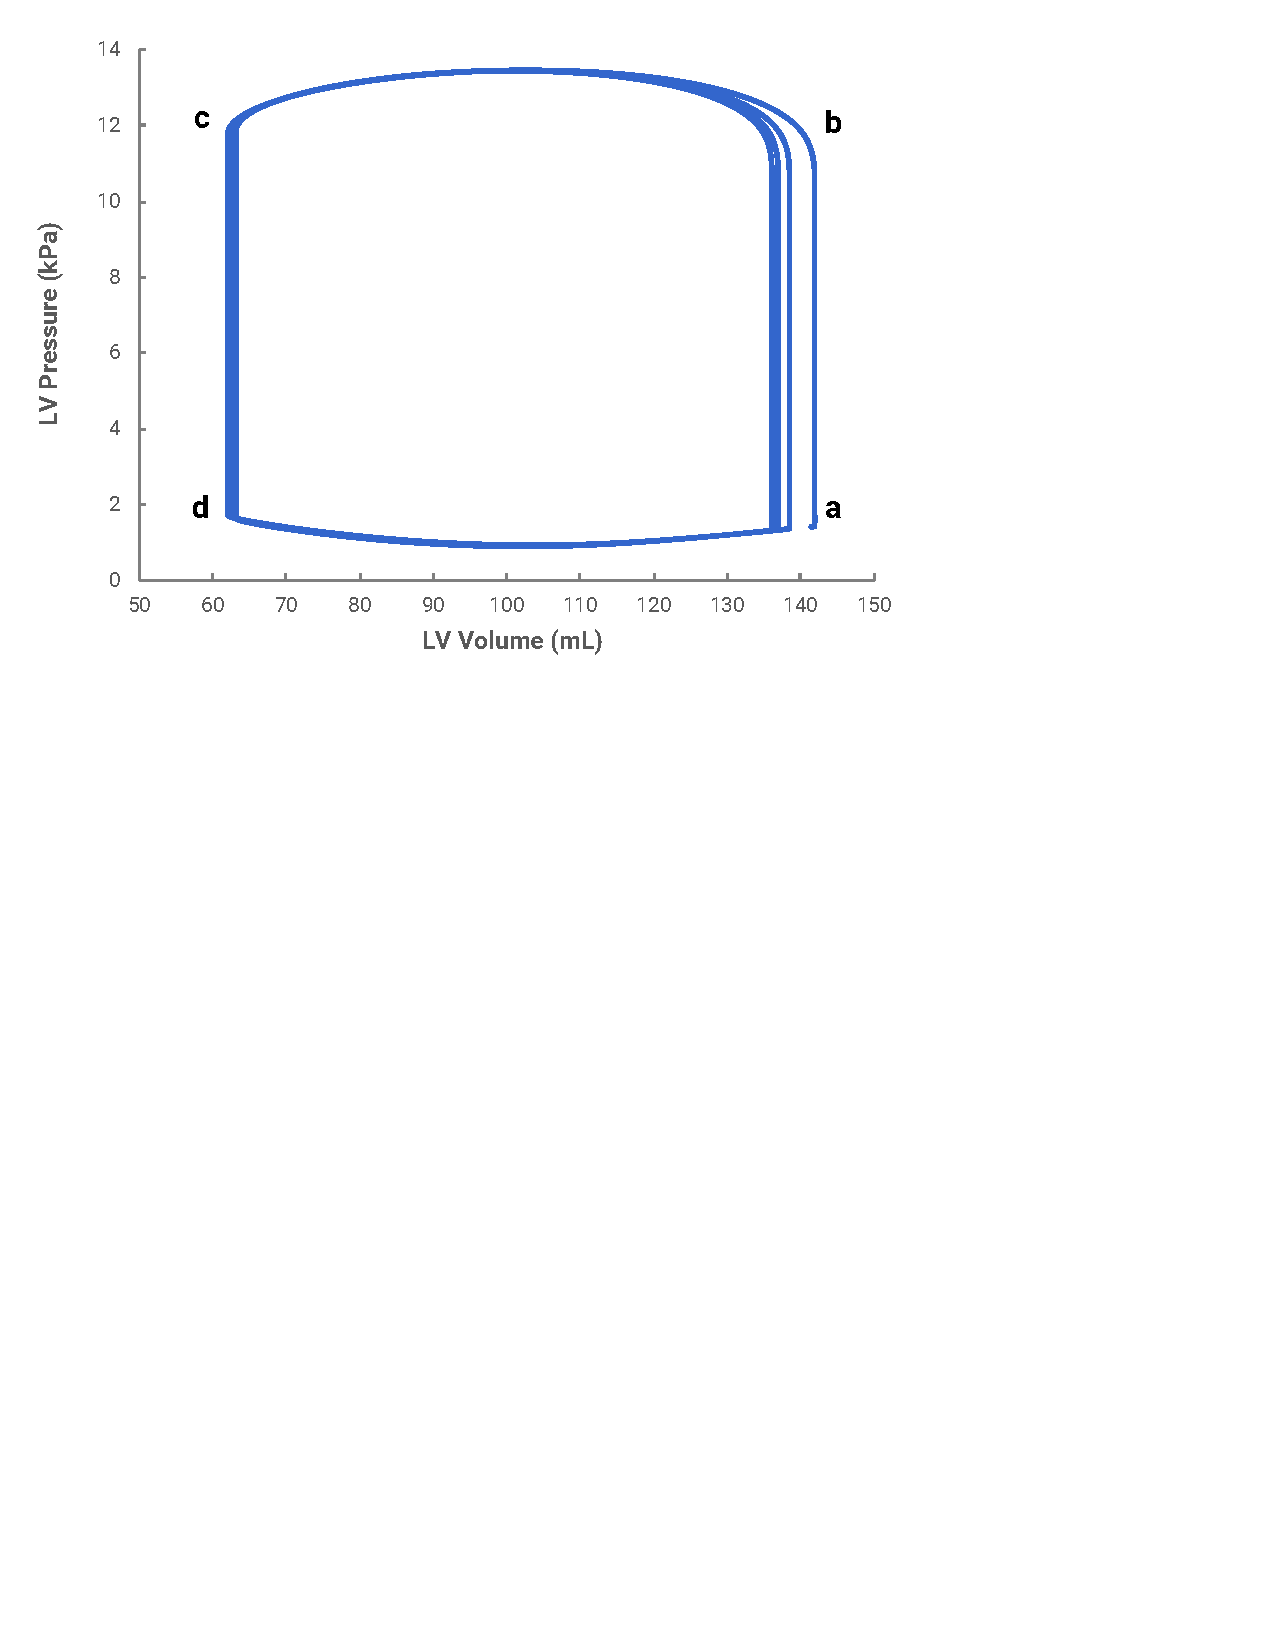
\includegraphics[scale=0.5]{media/4-cardioid/5-pv/pressure_volume-1.pdf}
\label{fig:pv1}}		
\subfigure[]{%
		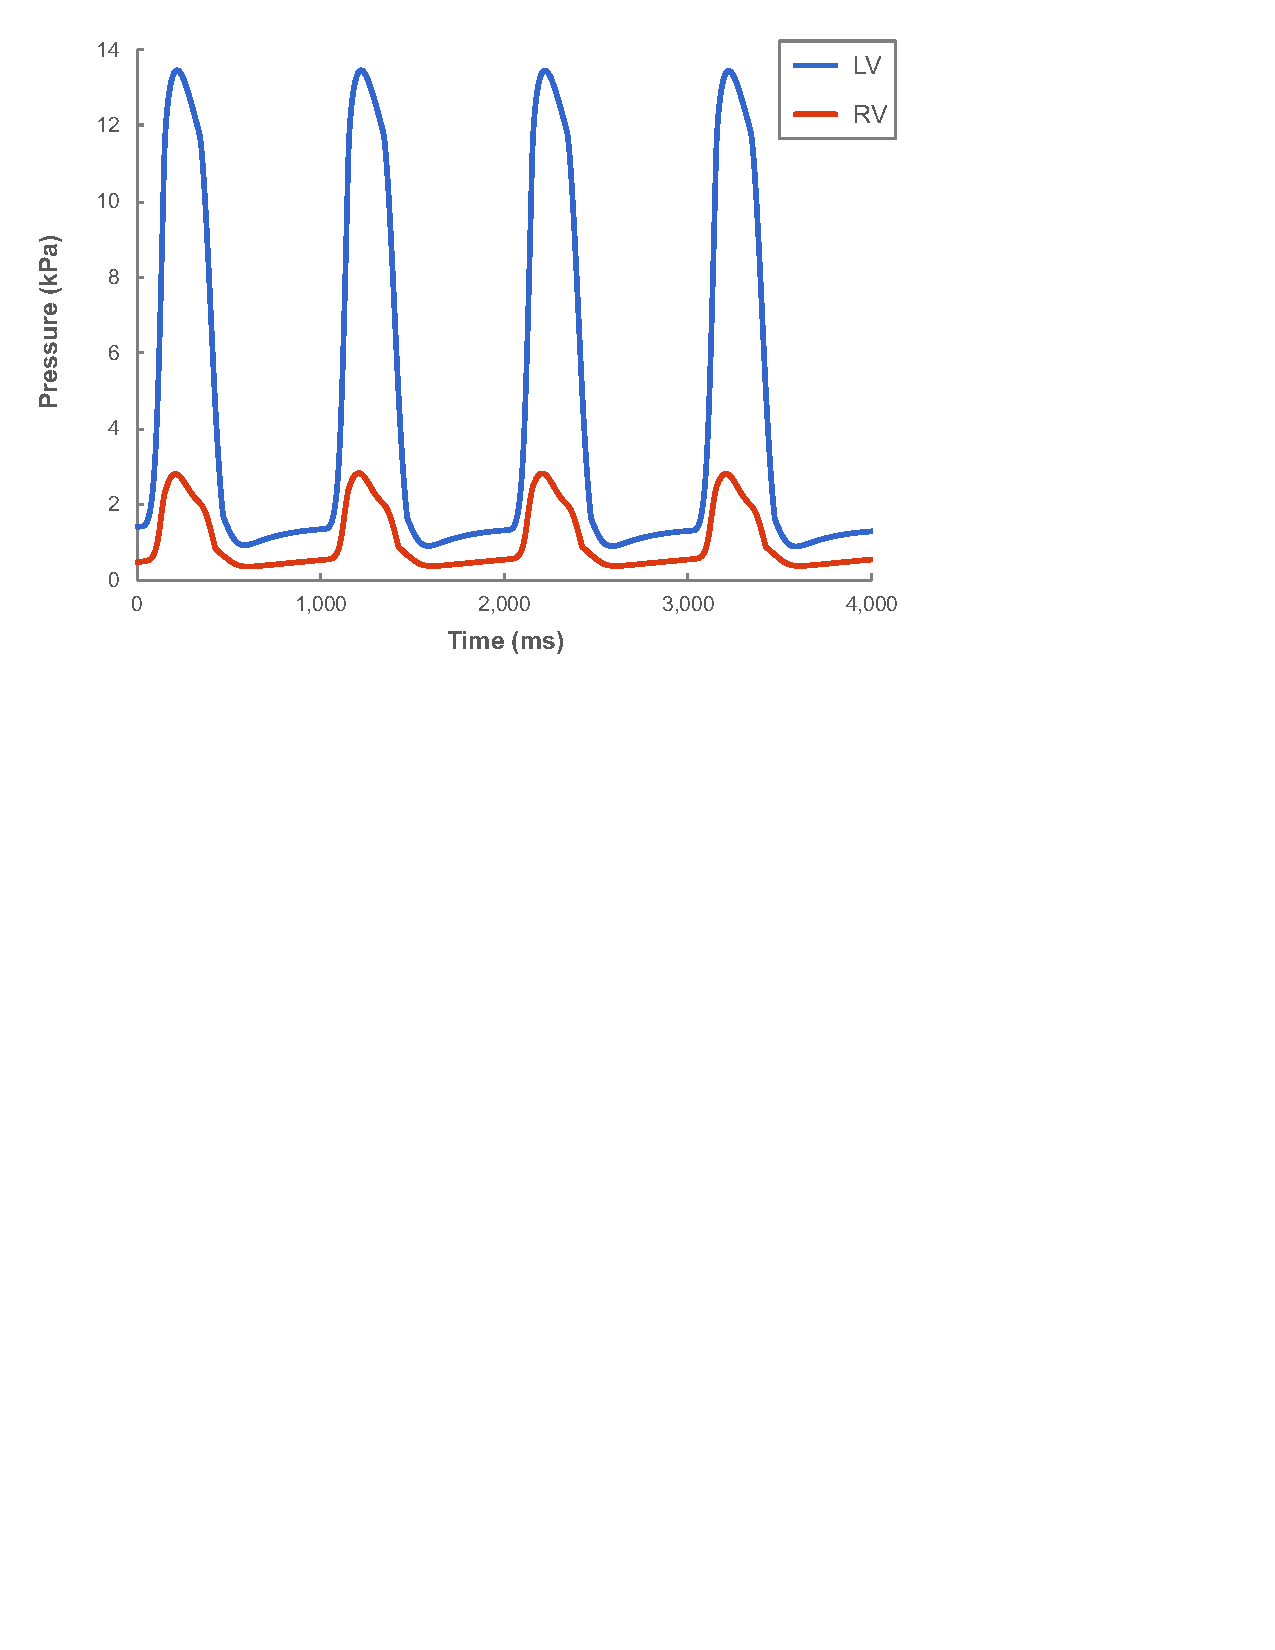
\includegraphics[scale=0.5]{media/4-cardioid/5-pv/pressure_volume-2.pdf}
\label{fig:pv2}}		
%
\caption{Results from Cardioid simulation: (a) P-V loop of left ventricle, (b) pressure time history in left and right ventricles.}
\label{fig:pv}
\end{figure}

\begin{sidewaysfigure}[htbp!]
\centering
\subfigure[]{%
		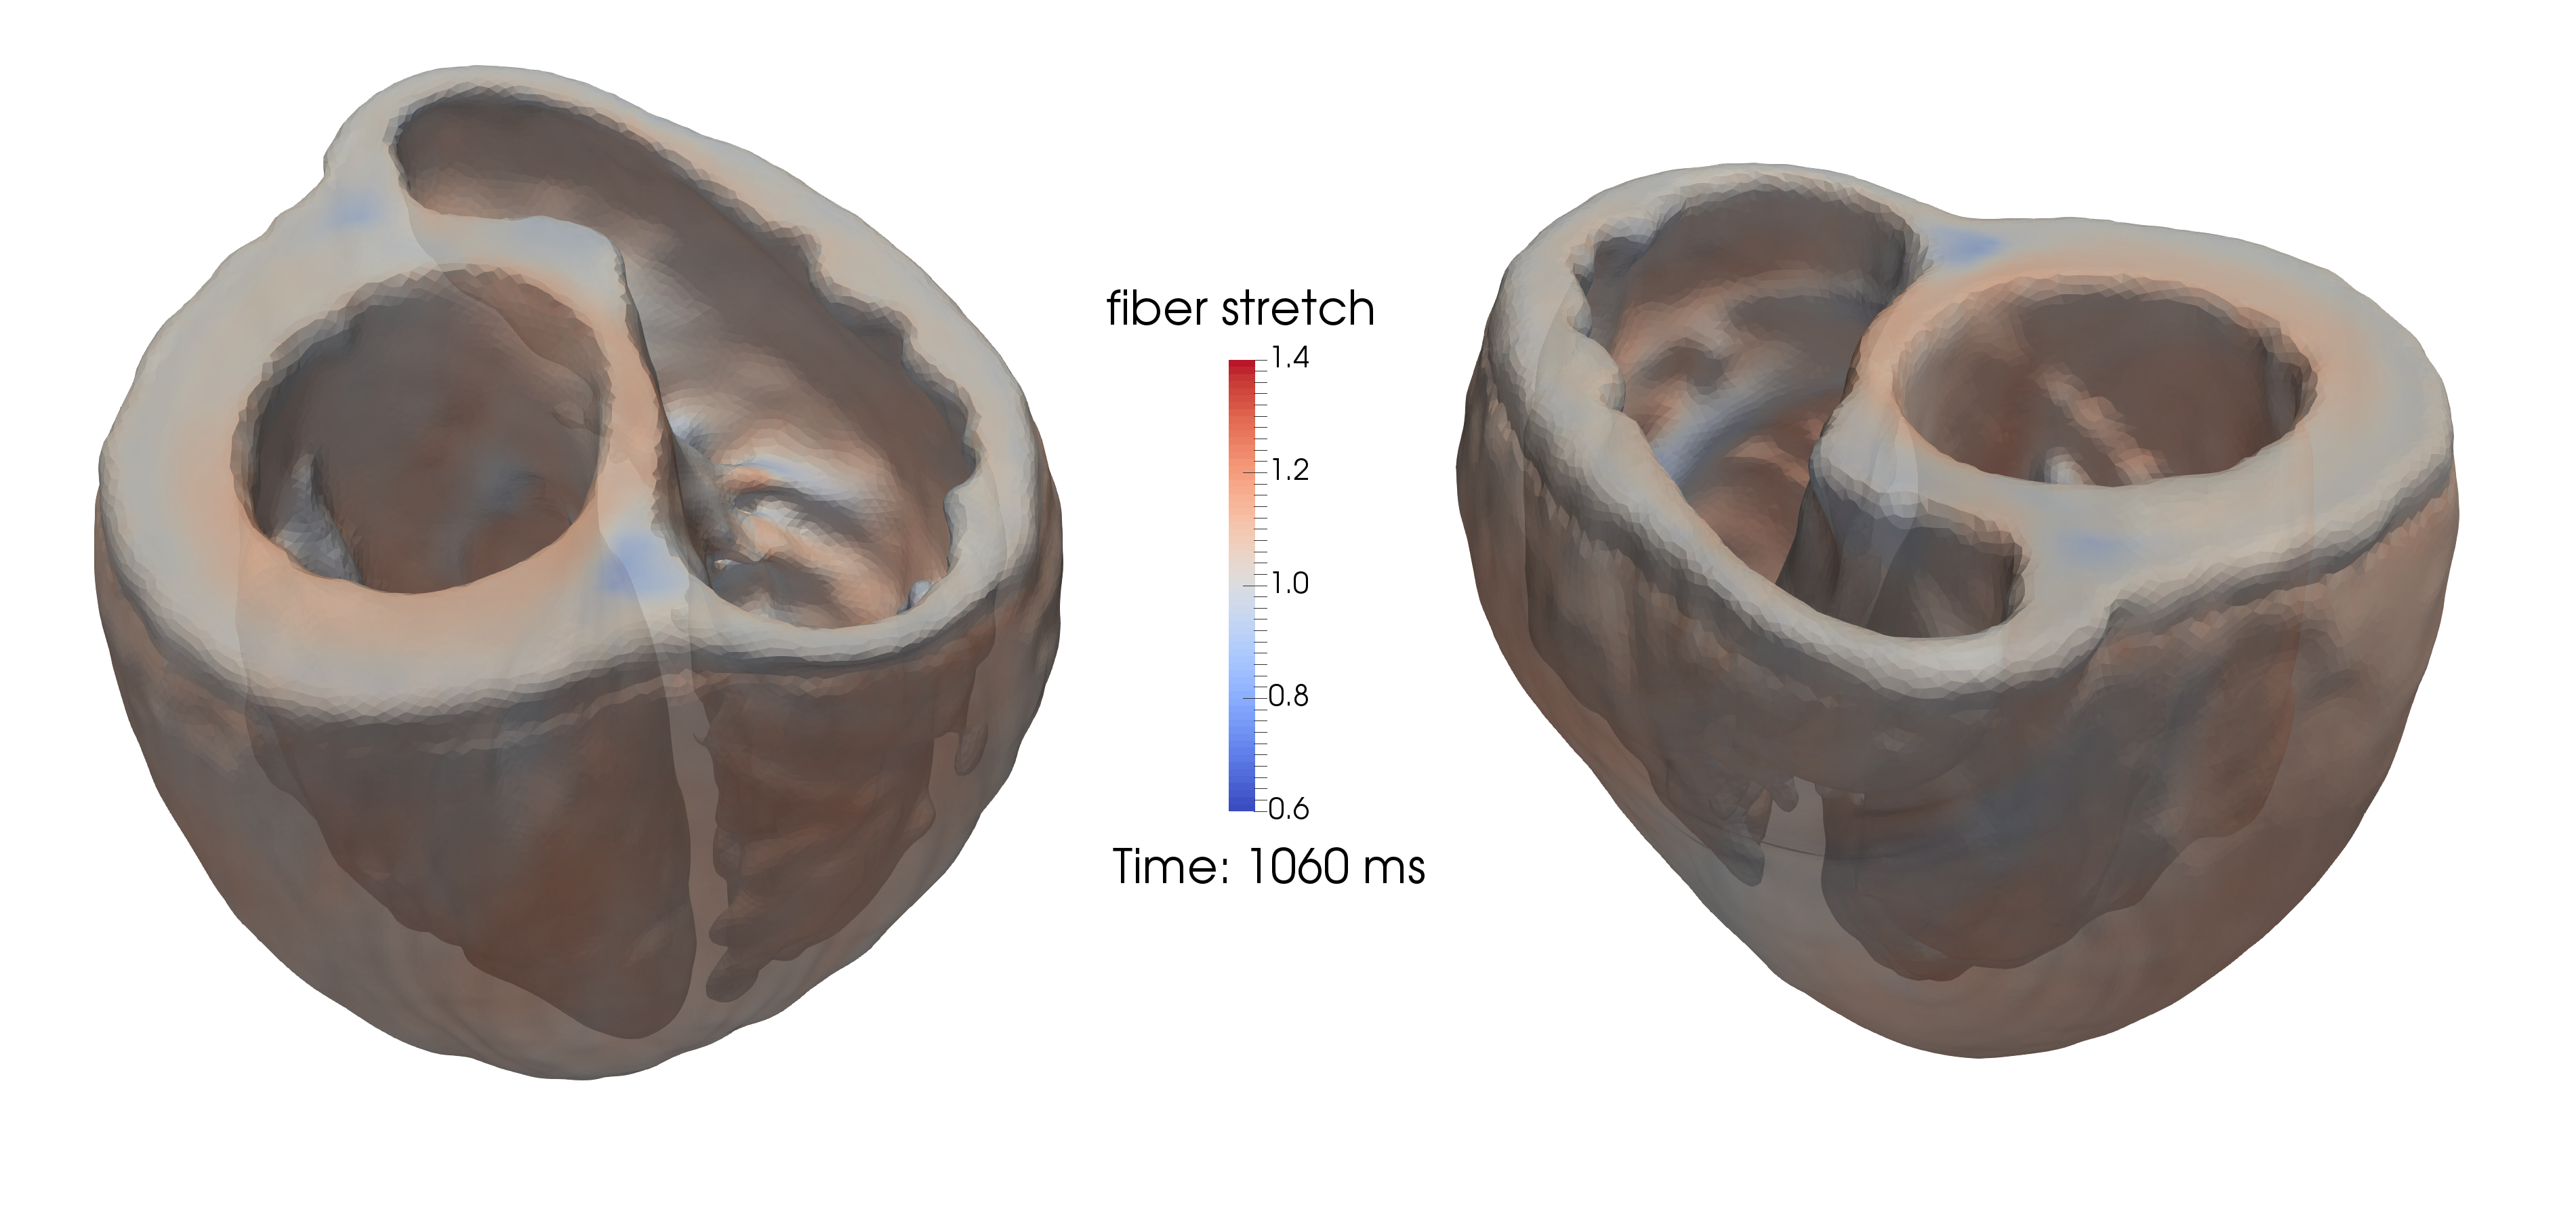
\includegraphics[scale=0.08]{media/4-cardioid/6-vid/a.png}
\label{fig:snaps1}}		
\subfigure[]{%
		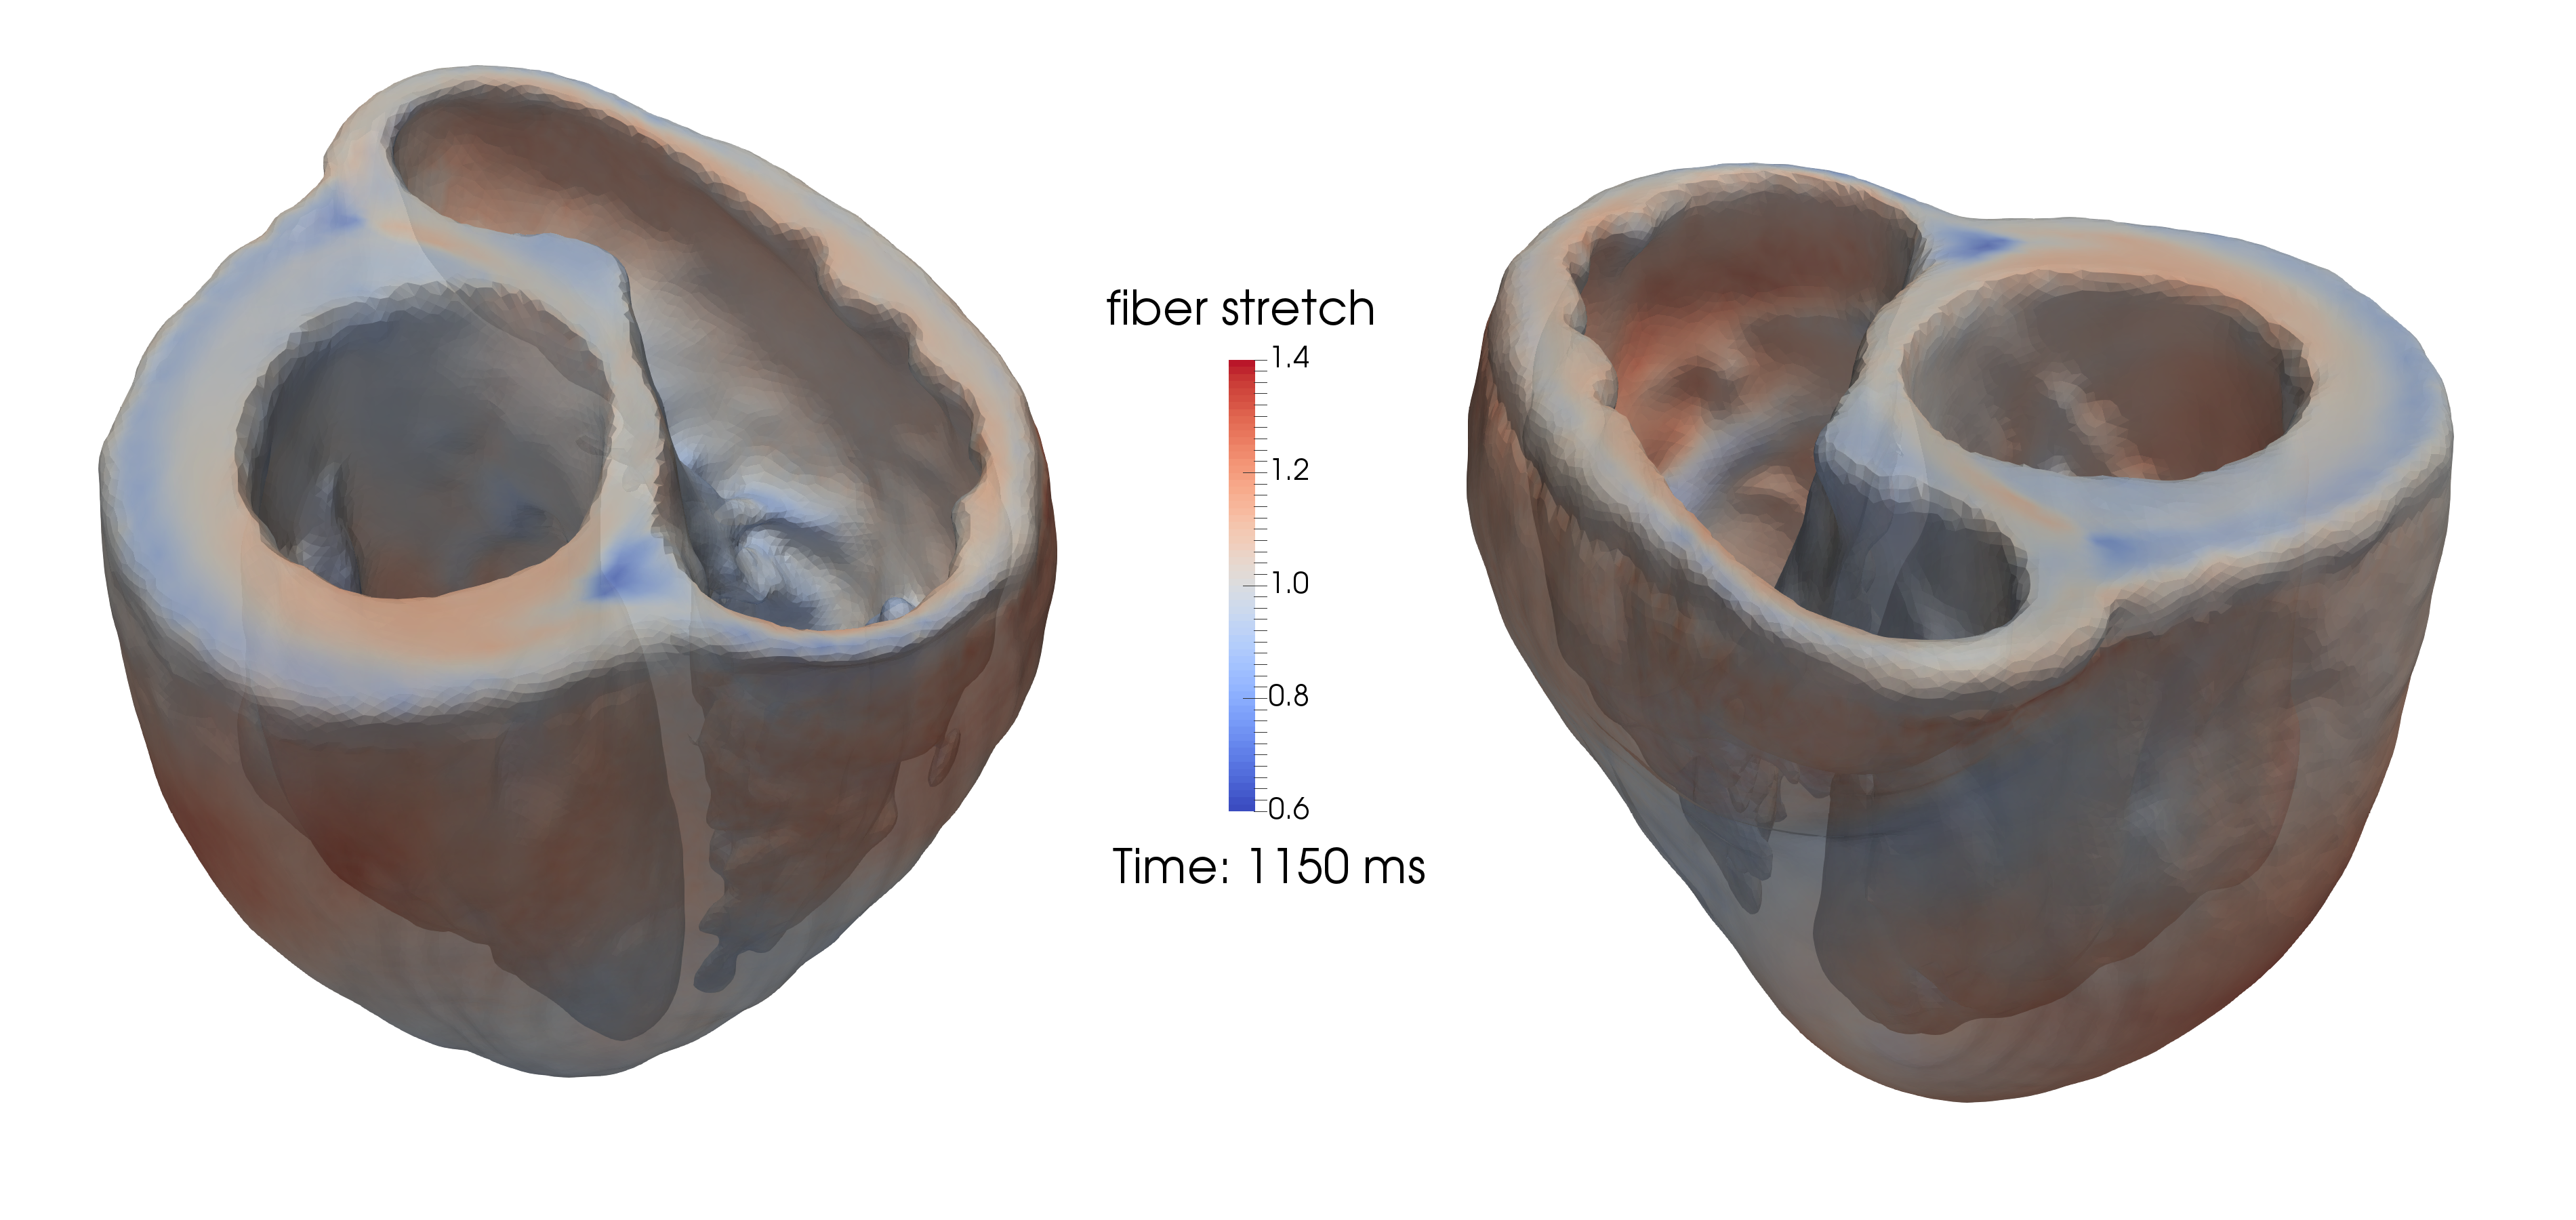
\includegraphics[scale=0.08]{media/4-cardioid/6-vid/b.png}
\label{fig:snaps2}}
\\
\subfigure[]{%
		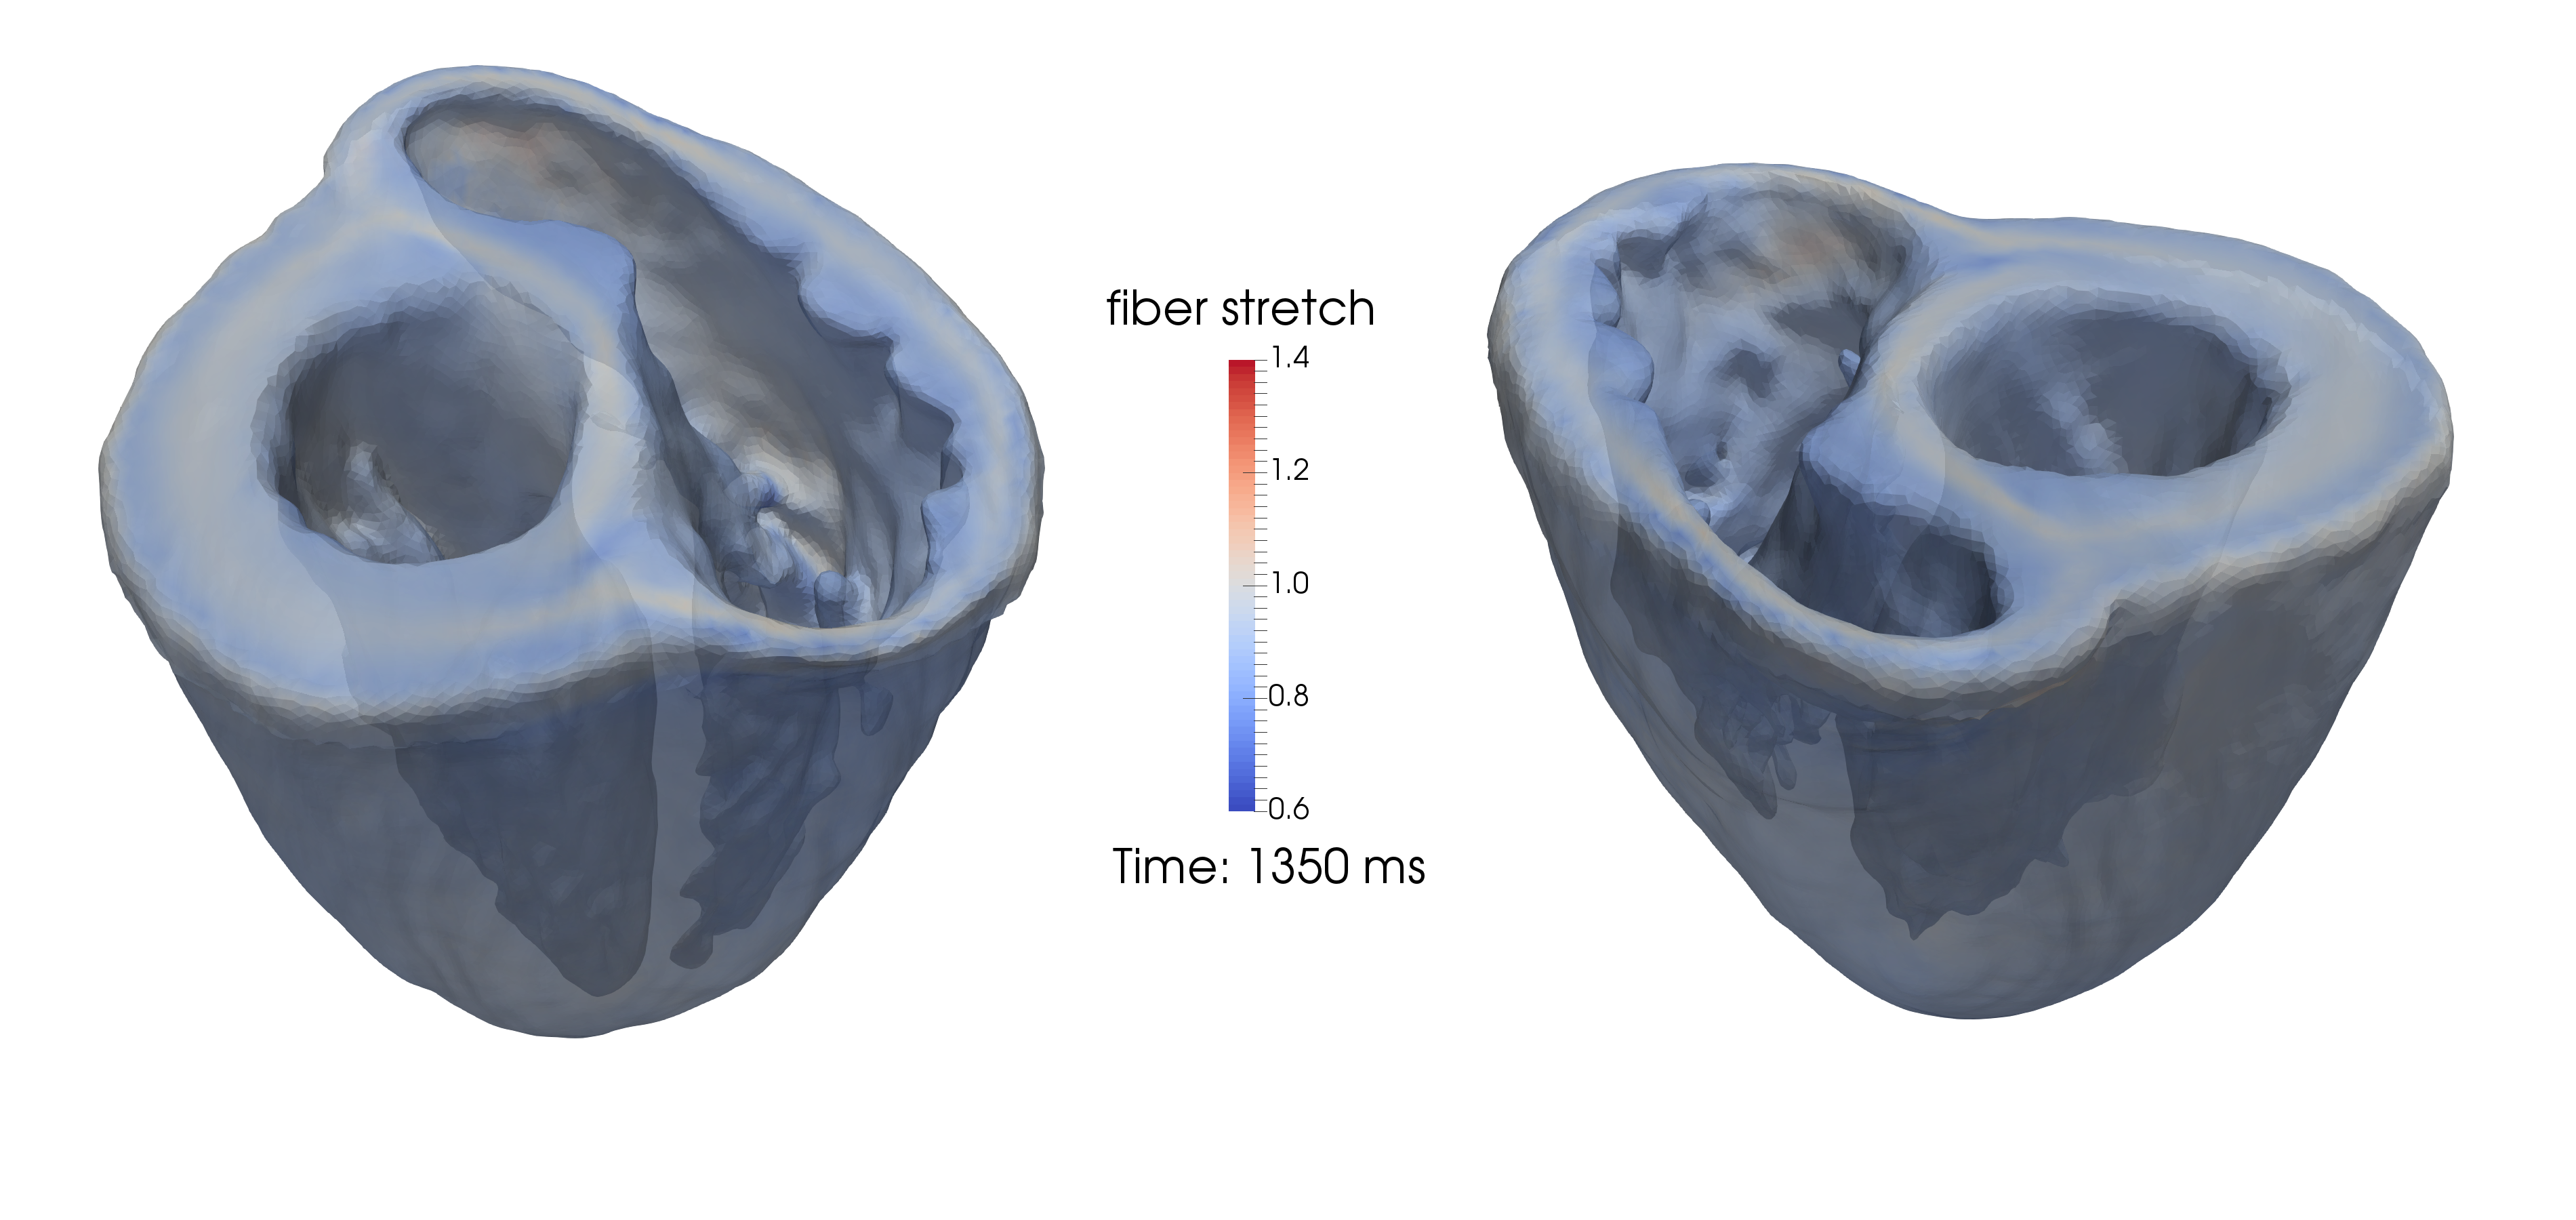
\includegraphics[scale=0.08]{media/4-cardioid/6-vid/c.png}
\label{fig:snapsf3}}		
\subfigure[]{%
		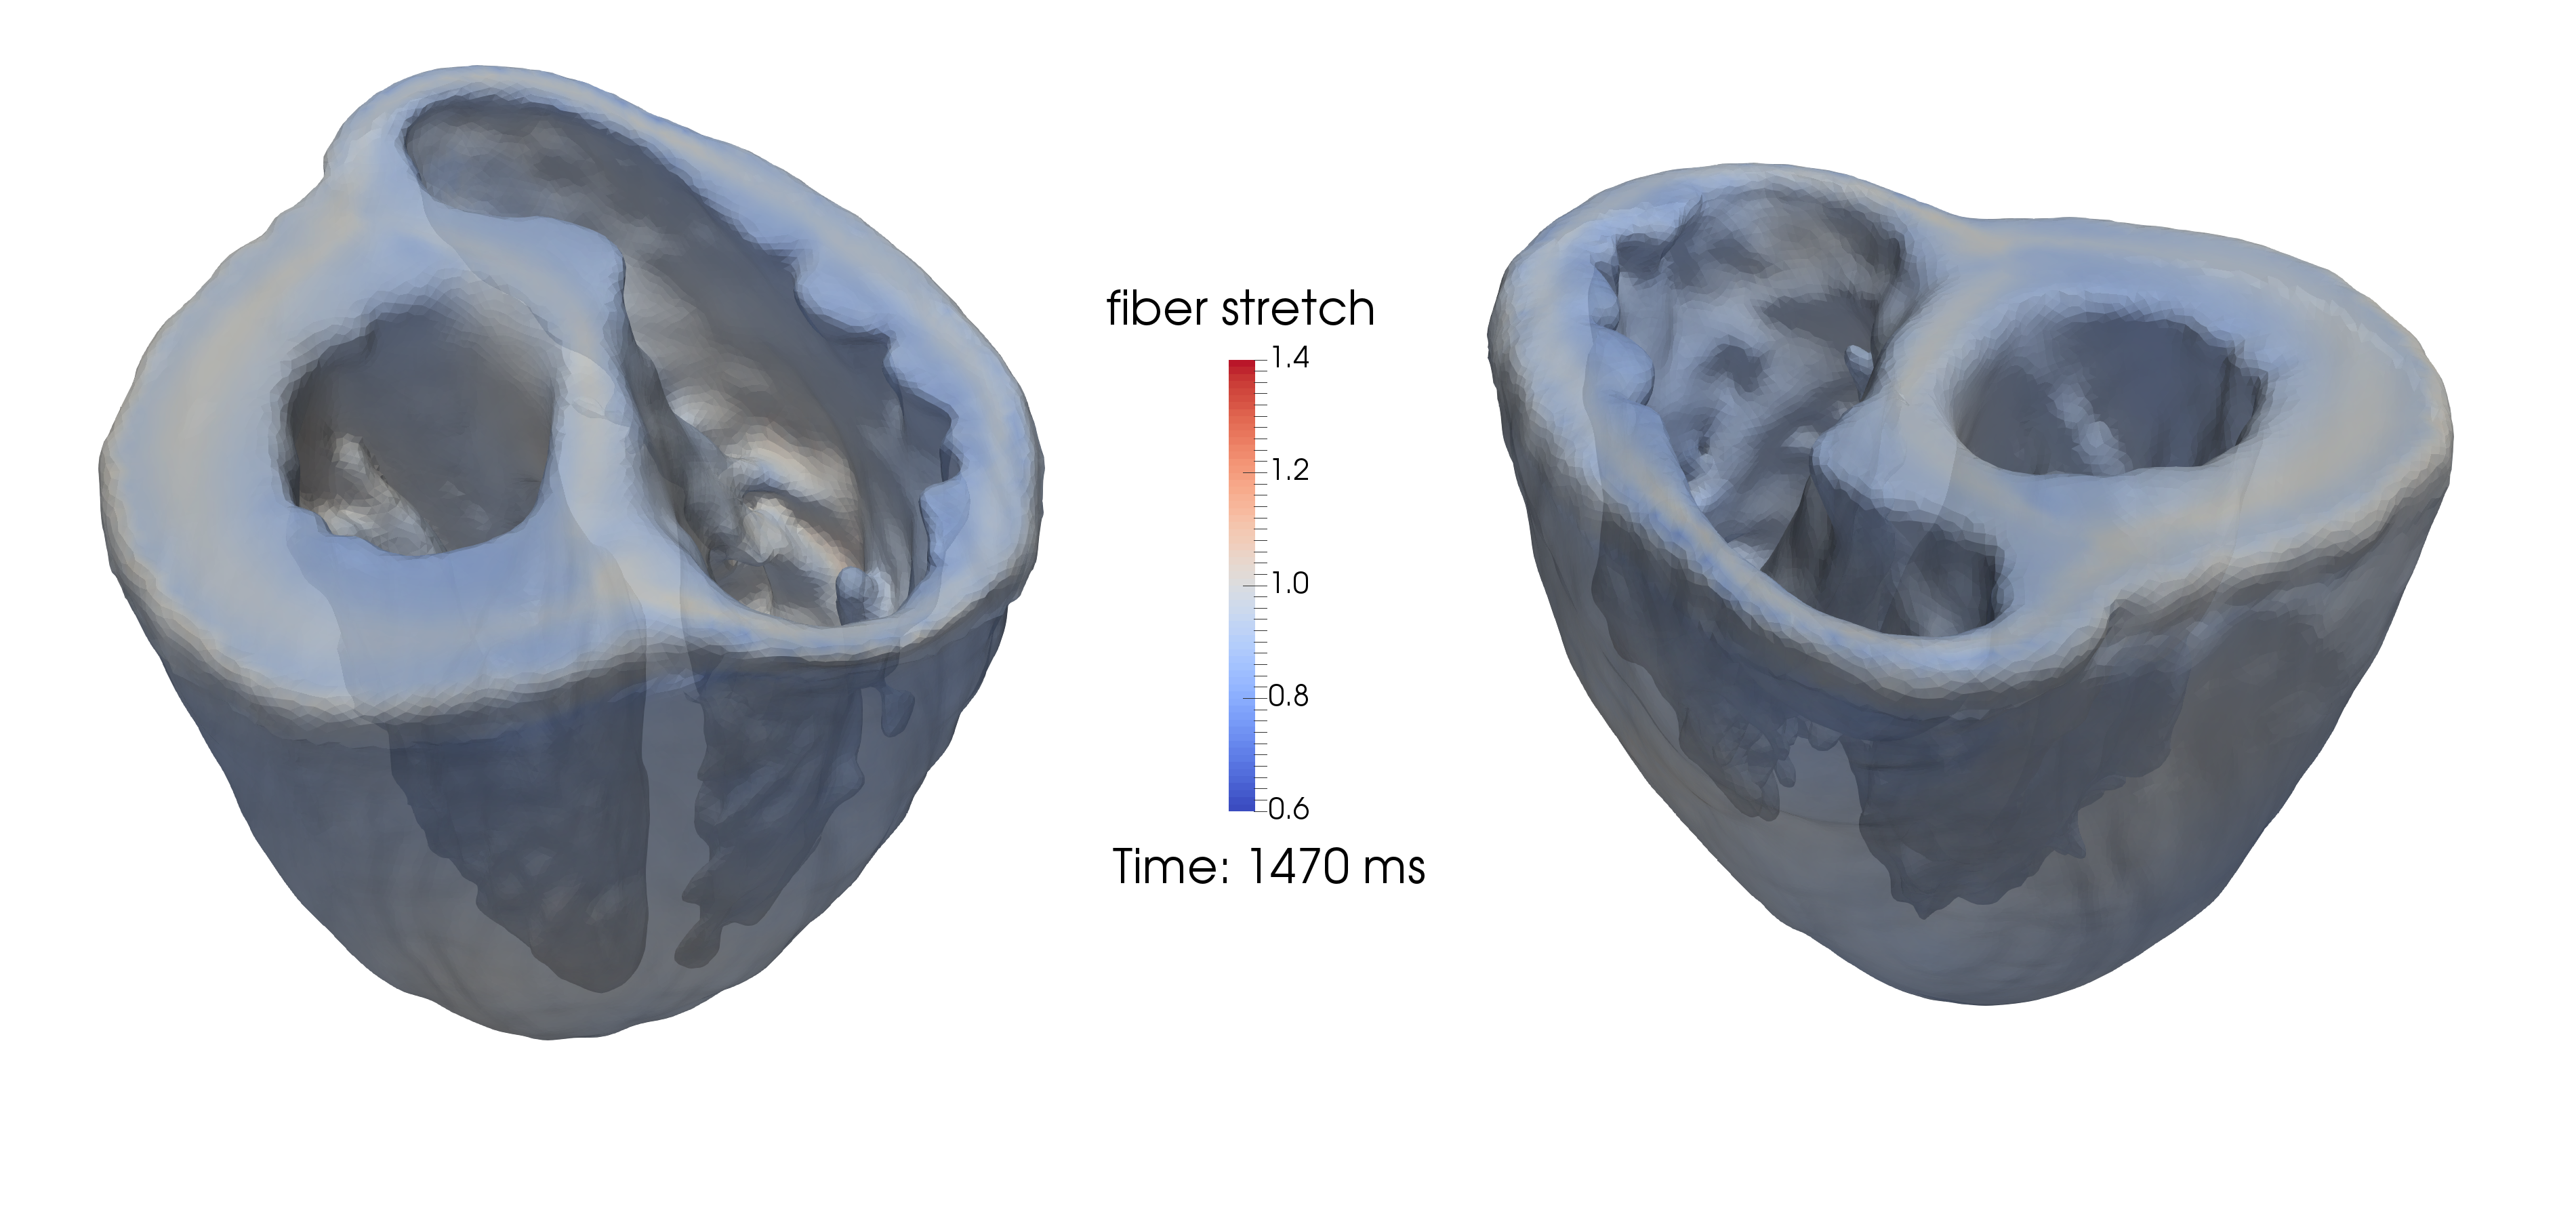
\includegraphics[scale=0.08]{media/4-cardioid/6-vid/d.png}
\label{fig:snaps4}}		
%
\caption{Deformed mesh from Cardioid simulation at different stages of cardiac cycle. Panels (a), (b), (c), and (d) correspond to the stages in the P-V loop denoted in~\figref{pv}.}
\label{fig:snaps}
\end{sidewaysfigure}

%%%%%%%%%%%%%%%%%%%%%%%%%%%%%%%%%%%%%%%%%%%%%%%
%%%%%%%%%%%%%%%%%%%%%%%%%%%%%%%%%%%%%%%%%%%%%%%
\section{Extension to Polyhedral Finite Elements}
\label{Polyhedral Finite Elements}

Efforts have been made to implement the mechanics described in this chapter into the polyhedral FEM code \textit{Celeris}. The details of the implementation will be discussed, followed by a showcase of cardiac verification results using polyhedral finite elements.

\subsection{Implementation}

The same surface mesh used to produce the quadratic tetrahedral mesh for Cardioid is used to produce the polyhedral mesh in Celeris, shown in \figref{cel}. As mentioned in \chapref{3}, a significant reduction in the number of degrees of freedom is exhibited in comparison to the quadratic tet mesh used for Cardioid. The fiber orientations, activation times, and surface tags are generated using Cardioid and subsequently read into Celeris for use. The Dirichlet boundary conditions applied in Cardioid are applied in Celeris using the same surface tags shown in \figref{supp3}. For simplicity, the ventricular pressure time histories from the Cardioid simulation are used directly for the imposition of ventricular boundary conditions in Celeris, rather than imposing volume constraints as described previously. The Cauchy pressure time histories $p_{LV}(t)$ and $p_{RV}(t)$ are sufficient in demonstrating an image-based polyhedral FEM workflow. Of course, in the future the volume constraint would be implemented as well so that the Celeris mechanics code is completely independent of the Cardioid mechanics results. 

The remaining consideration to perform cardiac simulations using polyhedral FEM is the implementation of the constitutive update.

\subsubsection{Material Model}
The Usyk material model is implemented within the Celeris framework. Rather than full incompressibility via a mixed pressure-displacement formulation, \textit{near-incompressibility} is enforced via a penalty term in the strain energy for volumetric material response, together with an \textit{F-bar projection method}. Regarding the penalty term, the strain energy is defined in the following manner, as is done by Usyk \textit{et al.}~\cite{usyk_2002}:
\begin{equation}
W = \frac{C}{2}\left(e^Q -1\right) + C_{compr} (J \cdot \ln J - J + 1) \\
\end{equation}
The parameter $C_{compr}$ is defined such that the volumetric response of the material is significantly stiffer than the deviatoric response. It was found that a value of $C_{compr} \geq 200  C$ gives good results (compared to simulations enforcing full incompressibility) without significantly making the system poorly conditioned. Near-incompressibility is then enforced by an F-bar projection method, in which the deformation gradient is modified such that the dilatation $det(\bm{F})$ at each integration point is replaced by a constant element-averaged value, as explained in detail by Doll~\textit{et al.}~\cite{doll_2000}.

\textbf{Passive stress}

The material model framework in Celeris currently accepts material definitions in \textit{incremental form}. The incremental material model receives as input: the beginning step Cauchy stress $\overline{\bm{T}}$, beginning step state variables $\overline{\bm{s}}$, strain rate $\bm{D}$, and material properties and other field parameters. Following the constitutive update, the model produces as output: the end step unrotated Cauchy stress $\tilde{\bm{T}}$, end step unrotated state variables $\tilde{\bm{s}}$, and end step tangent modulus $\frac{\partial \tilde{\bm{T}}}{\partial (\bm{D}\Delta{t})}$. However, hyperelastic materials are generally defined as functions of the deformation gradient $\bm{F}$, not of the strain rate $\bm{D}$. As is done in \chapref{4} for the Mooney-Rivlin material, it is assumed that $\hat{\bm{U}} = \text{exp}(\bm{D}\Delta{t})$, which is approximated using its Taylor expansion.

The beginning step deformation gradient $\overline{\bm{F}}$ is stored as a state variable to accommodate the incremental material form. Thus, the state variables $\bm{s}$ are comprised of $\overline{\bm{F}}$ and the active tension model state variables $\bm{w}$. Material parameters were previously defined in \eqnref{usyk}. The field parameters at each integration point are the fiber transformation matrix $\bm{Q}$ and activation time $t_a$. Both quantities are computed using Cardioid \textit{a priori} and are imported into Celeris at the integration points. It is important to distinguish between the \textit{transformation matrix} $\bm{Q}$ from the global to local fiber coordinate frames, and the \textit{rotation increment} $\hat{\bm{R}}$ that comprises the rotation portion of the incremental deformation gradient $\hat{\bm{F}}$. Lastly, the material model admits the beat duration $t_b$ and the beginning and end step times $t_n$ and $t_{n+1}$, which are used for the calculation of active stress.

Because of the assumed additive stress decomposition $\tilde{\bm{T}} = \tilde{\bm{T}}_p + \tilde{\bm{T}}_a$, the passive and active stress are computed independently and then added together at the end of the constitutive update. The passive material update proceeds as follows: 1) the end step unrotated deformation gradient is calculated as $\tilde{\bm{F}} = \hat{\bm{U}}\bm{F}$, 2) the deformation gradient $\tilde{\bm{F}}$ is transformed into the local fiber coordinate system as $\tilde{\bm{F}}'$, 3) the end step unrotated Cauchy stress in the local fiber coordinate system $\tilde{\bm{T}}'$ is computed based on $\tilde{\bm{F}}'$, and finally 4) the stress is transformed back into the global coordinate frame as the desired quantity $\tilde{\bm{T}}$. The ``prime'' here corresponds to the tensor of interest being expressed as a matrix in the local fiber coordinate frame. The computations proceed in the following manner:
\begin{equation}
\hat{\bm{U}} = \bm{I} + \bm{D}\Delta{t} + \frac{1}{2}(\bm{D}\Delta{t})^2 + \frac{1}{6}(\bm{D}\Delta{t})^3
\end{equation}
\begin{align}
\tilde{\bm{F}} &= \hat{\bm{U}}\bm{F} \\
\tilde{\bm{F}}' &= \bm{Q}^T\tilde{\bm{F}}\bm{Q} \\
\bm{C}' &= \tilde{\bm{F}}'^T \tilde{\bm{F}}' \\
\bm{E}' &= \frac{1}{2}(\bm{C}' - \bm{I}) \\
J  &= \det{\tilde{\bm{F}}'}
\end{align}
\begin{equation}
\begin{aligned}
Q' &= b_{ff} E'^2_{ff} + b_{ss} E'^2_{ss} + b_{nn} E'^2_{nn} + \\
&\text{\ \ \ }b_{fs}\left(E'^2_{fs} + E'^2_{sf}\right) + b_{fn}\left(E'^2_{fn} + E'^2_{nf}\right) + b_{ns}\left(E'^2_{ns} + E'^2_{sn}\right)
\end{aligned}
\end{equation}
\begin{align}
N_{pq} &= 2 \left[\begin{array} {ccc} b_{ff} & b_{fs} & b_{fn} \\ b_{fs} & b_{ss} & b_{sn} \\ b_{fn} & b_{sn} & b_{nn} \end{array} \right] \\
\frac{\partial Q'}{\partial \bm{E}'} &= \bm{N} \circ \bm{E}' \\
\tilde{\bm{T}}' &= \frac{C}{2J}e^{Q'}\tilde{\bm{F}}'\frac{\partial{Q'}}{\partial{\bm{E}'}}\tilde{\bm{F}}'^T + (C_{comp}\text{ln}J)\bm{I} \\
\tilde{\bm{T}}_p &= \bm{Q} \tilde{\bm{T}}' \bm{Q}^T
\end{align}
Note the Cauchy stress is computed from the strain energy by making use of the relationship $\bm{T} = J^{-1}\bm{F}\frac{\partial\bm{W}}{\partial \bm{E}} \bm{F}^T$. The \textit{Hadamard} or \textit{entrywise product} is employed in defining $\frac{\partial Q'}{\partial \bm{E}'}$, namely $\frac{\partial Q'}{\partial E'_{pq}} = N_{pq}E'_{pq}$ with no implied sum on the indices. The sequence of calculations result in the desired end step unrotated passive Cauchy stress $\tilde{\bm{T}}_p$.

The tangent modulus of the passive portion of stress $\frac{\partial \tilde{\bm{T}}_p}{\partial (\bm{D}\Delta{t})}$ is computed via successive use of the chain rule of differentiation:
\begin{equation}
\frac{\partial \tilde{\bm{T}}_p}{\partial (\bm{D}\Delta{t})} = \frac{\partial \tilde{\bm{T}}_p}{\partial \tilde{\bm{T}'}}\frac{\partial \tilde{\bm{T}'}}{\partial \tilde{\bm{F}'}}\frac{\partial \tilde{\bm{F}'}}{\partial \tilde{\bm{F}}}\frac{\partial \tilde{\bm{F}}}{\partial \hat{\bm{U}}}\frac{\partial \hat{\bm{U}}}{\partial (\bm{D}\Delta{t})}
\label{eqn:tanmod}
\end{equation}

Each of the terms are defined below:
\begin{align}
\frac{\partial (\tilde{T}_p)_{ij}}{\partial \tilde{T}'_{mn}} &= \frac{1}{2}\left[Q'_{im}Q'_{jn} + Q'_{in}Q'_{jm}\right] \\
A_{pq} &\equiv \frac{\partial Q'}{\partial E'_{pq}} \\
Z_{pqkl} &\equiv \frac{1}{2}N_{pq}\left[F_{kq}\delta_{pl} + F_{kp}\delta_{ql}\right] \text{ (no sum)}
\end{align}
\begin{equation}
\begin{aligned}
\frac{\partial \tilde{T}'_{ij}}{\partial \tilde{F}'_{kl}} &= \frac{C}{2J}e^{Q'} \Bigg[-\tilde{F}'^{-1}_{lk}A_{pq}\tilde{F}'_{ip}\tilde{F}'_{jq} + \frac{1}{2}(A_{ln}\tilde{F}'_{kn} + A_{ml}\tilde{F}'_{km})A_{pq}\tilde{F}'_{ip}\tilde{F}'_{jq} + \\
&\text{\ \ \ }Z_{pqkl}\tilde{F}'_{ip}\tilde{F}'_{jq} + \delta_{ik}A_{pl}\tilde{F}'_{jp} + \delta_{jk}A_{lq}\tilde{F}'_{iq}\Bigg] + C_{comp}\delta_{ij}\tilde{F}'^{-1}_{lk}
\end{aligned}
\end{equation}
\begin{align}
\frac{\partial \tilde{F}'_{ij}}{\partial \tilde{F}_{mn}} &= Q'_{mi}Q'_{nj} \\
\frac{\partial \tilde{F}_{ij}}{\partial \hat{U}_{kl}} &= \frac{1}{2}\left[\delta_{ik}\overline{F}_{lj} + \delta_{il}\overline{F}_{kj}\right]
\end{align}
\begin{equation}
\begin{aligned}
\frac{\partial \hat{U}_{ij}}{\partial D_{kl}} = &\frac{1}{2}\left[\delta_{ik}\delta_{jl} + \frac{1}{2}\delta_{ik}D_{lj} + \frac{1}{2}D_{ik}\delta_{jl} + \frac{1}{6}\delta_{ik}D_{ln}D_{nj} + \frac{1}{6}D_{ik}D_{lj} + \frac{1}{6}D_{im}D_{mk}\delta_{jl}\right] + \\
&\frac{1}{2}\left[\delta_{il}\delta_{jk} + \frac{1}{2}\delta_{il}D_{kj} + \frac{1}{2}D_{il}\delta_{jk} + \frac{1}{6}\delta_{il}D_{kn}D_{nj} + \frac{1}{6}D_{il}D_{kj} + \frac{1}{6}D_{im}D_{ml}\delta_{jk}\right]
\end{aligned}
\end{equation}
Again, the derivatives are then combined to produce the tangent modulus defined in \eqnref{tanmod}.

The passive material model has been implemented, and the computed stress and corresponding tangent modulus have been thoroughly verified against finite difference approximations for accurate and quickly converging solutions.

\textbf{Active stress}

%%%%%%%%%%%%%%%%%%%%%%%%%%%%%%%%%%%%%%%%%%%%%%%%%%
The Fortran code to compute the active stress $\tilde{\bm{T}}_a$ and corresponding tangent modulus $\frac{\partial \tilde{\bm{T}}_a}{\partial (\bm{D}\Delta{t})}$ is generated using the Cardioid tool \textit{Melodee}~\cite{melodee}, a new language for expressing systems of ODEs that generates optimized code for various languages and platforms. Melodee has been tested and verified to generate a working Fortran subroutine for the Lumens active stress model.

Finally, the passive and active stress, along with their tangent moduli, are combined in the following manner:
\begin{align}
\tilde{\bm{T}} &= \tilde{\bm{T}}_p + \tilde{\bm{T}}_a \\
\frac{\partial \tilde{\bm{T}}}{\partial (\bm{D}\Delta{t})} &= \frac{\partial \tilde{\bm{T}}_p}{\partial (\bm{D}\Delta{t})}+ \frac{\partial \tilde{\bm{T}}_a}{\partial (\bm{D}\Delta{t})}
\end{align}

Following the constitutive update routine, the end step Cauchy stress and tangent modulus are forward rotated as discussed in \chapref{4}. Additionally, the state variable $\bm{F}$ is forward rotated simply via $\bm{F} =\hat{\bm{R}}\tilde{\bm{F}}$.

%%%%%%%%%%%%%%%%%%%%%%%%%%%%%%%%%%%%%%%%%%%%%%%%%%%%%%%%
%%%%%%%%%%%%%%%%%%%%%%%%%%%%%%%%%%%%%%%%%%%%%%%%%%%%%%%%

\subsection{Verification}

All compoenents required to perform a complete cardiac simulation have been implemented. Prior to running a complete cardiac simulation, the polyhedral workflow was tested for a suite of verification problems. Six verification problems were identified: three from Gurev \textit{et al.}~\cite{gurev_2015} and three from Land \textit{et al.}~\cite{land_2015}. The specifics of those problems can be found in the those papers. See \figref{beams} and \figref{ventricles} for the nomenclature used to identify the problems, as well as the type of mechanics being tested for each one.

\begin{figure}[ht]
\centering
\subfigure[]{%
		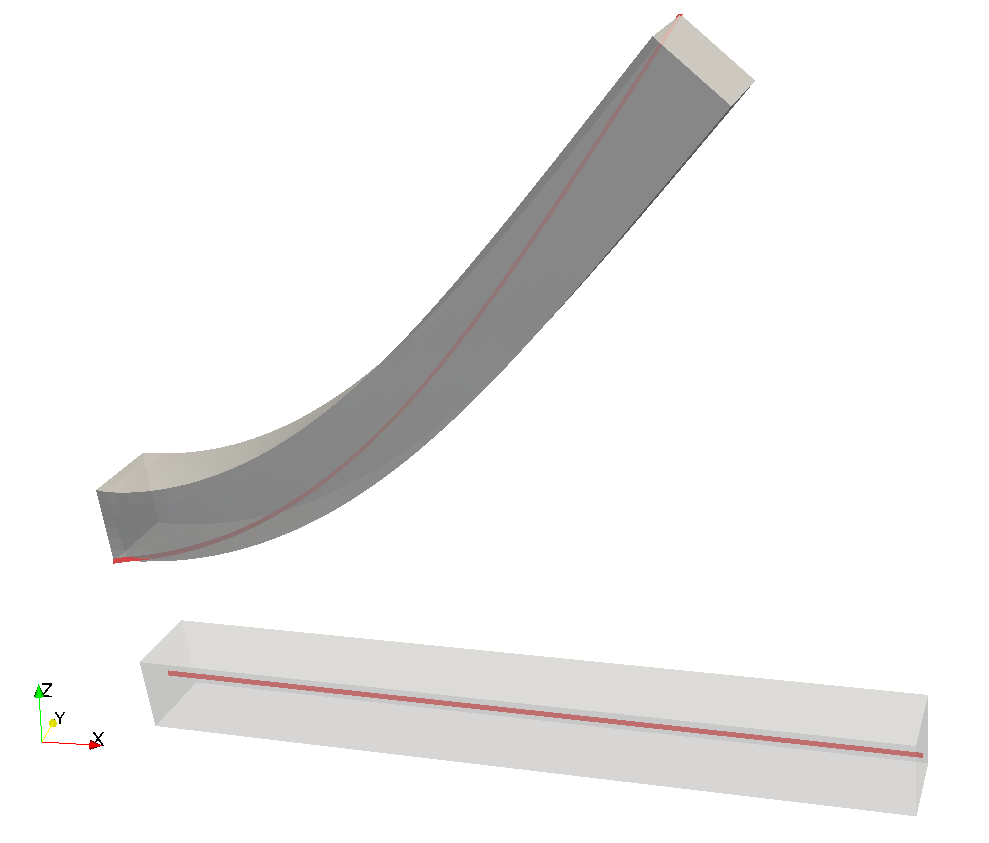
\includegraphics[scale=0.18]{media/5-verif/1-gurev2/gurev2.png}
\label{fig:beams1}}		
\subfigure[]{%
		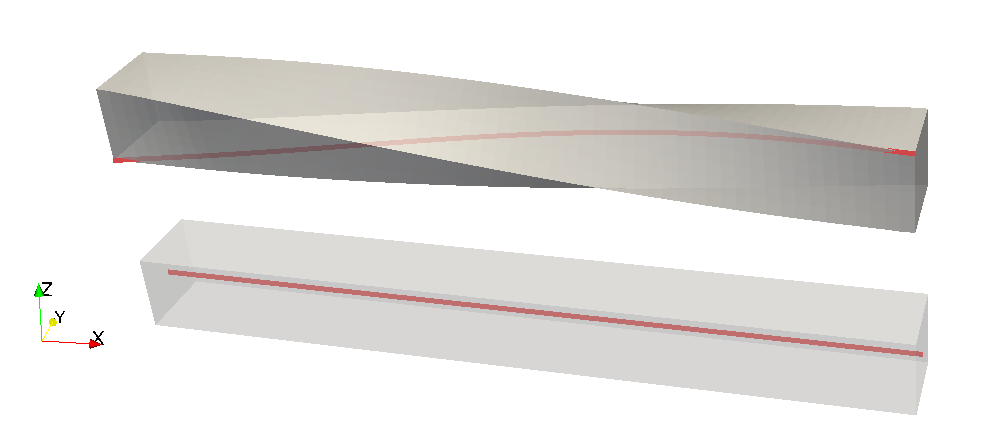
\includegraphics[scale=0.18]{media/5-verif/2-gurev3/gurev3.png}
\label{fig:beams2}}		
\subfigure[]{%
		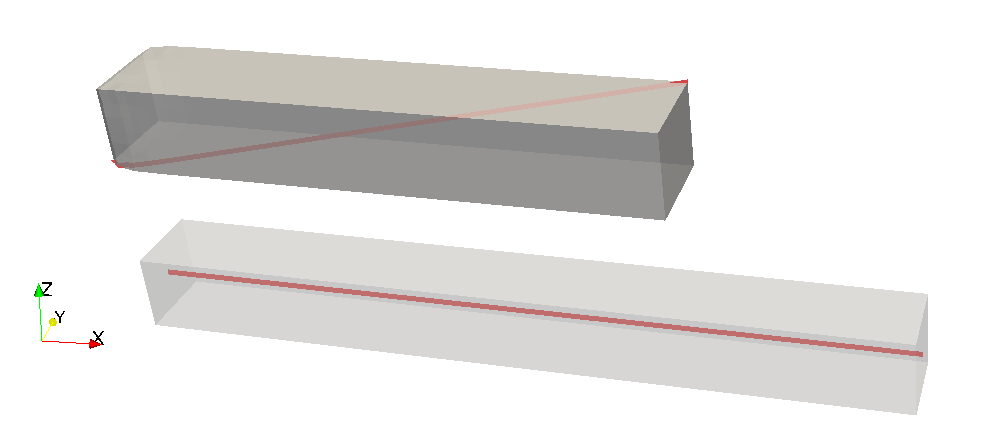
\includegraphics[scale=0.18]{media/5-verif/3-gurev4/gurev4.png}
\label{fig:beams3}}		
\subfigure[]{%
		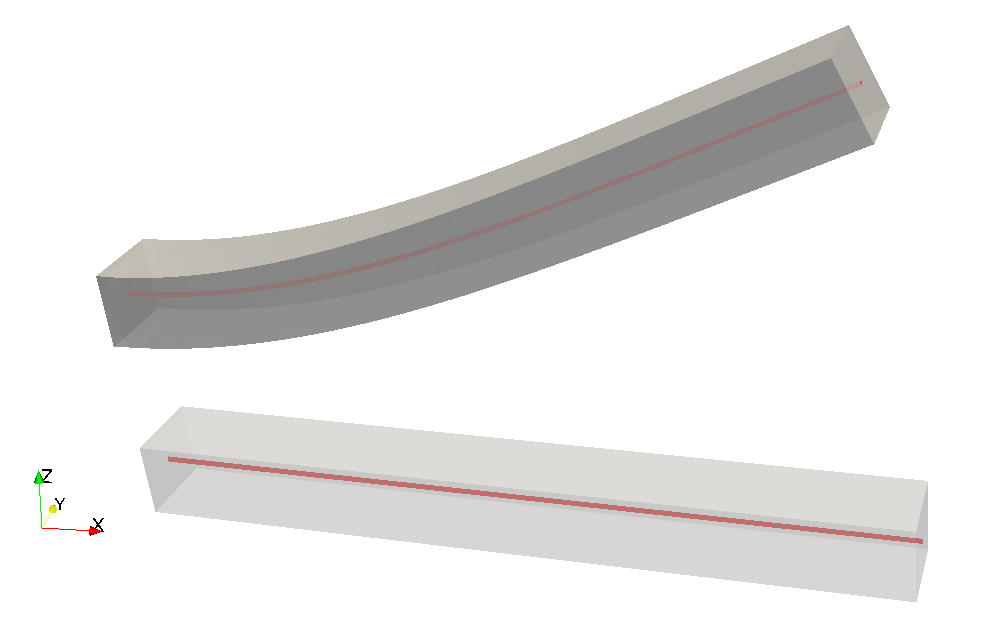
\includegraphics[scale=0.18]{media/5-verif/4-land1/land1.png}
\label{fig:beams4}}		
%
\caption{Undeformed (bottom) and deformed (top) configurations for cantilever beam verification problems: (a) Gurev P2: bending, (b) Gurev P3: torsion, c) Gurev P4: active contraction, and (d) Land P1: bending. The red curve denotes the curve over which displacements and positions are recorded and compared.}
\label{fig:beams}
\end{figure}

\begin{figure}[ht]
\centering
\subfigure[]{%
		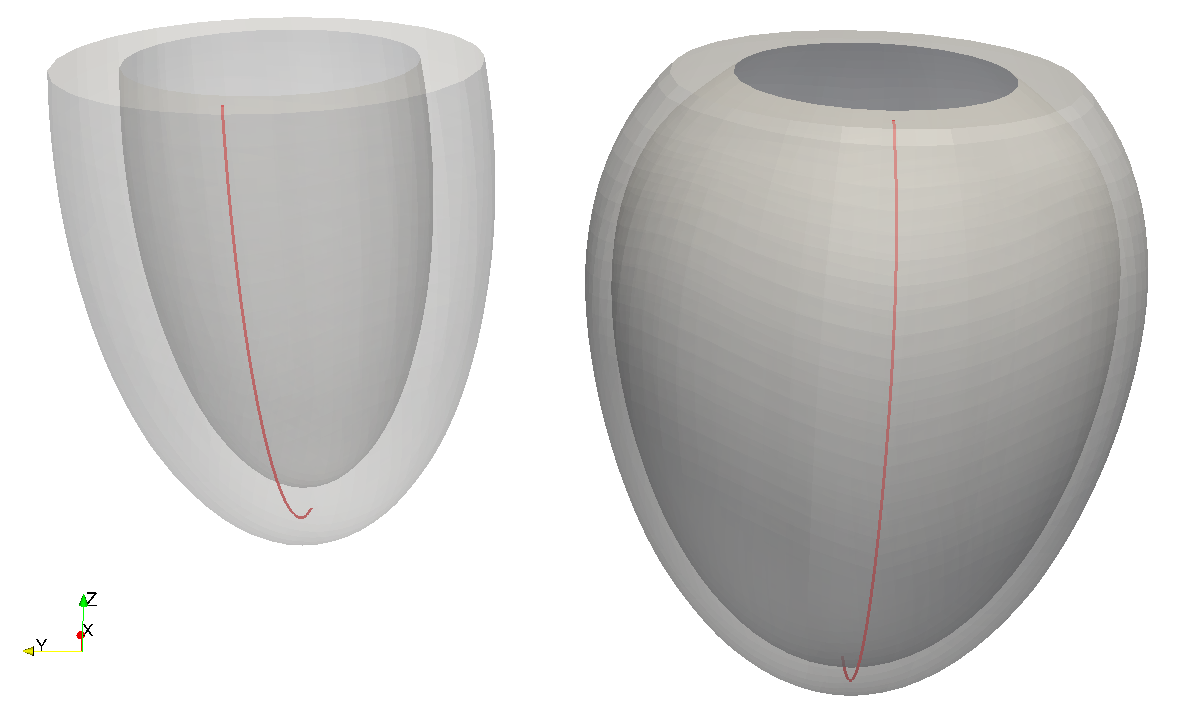
\includegraphics[scale=0.18]{media/5-verif/5-land2/land2-1.png}
\label{fig:ventricles1}}		
\subfigure[]{%
		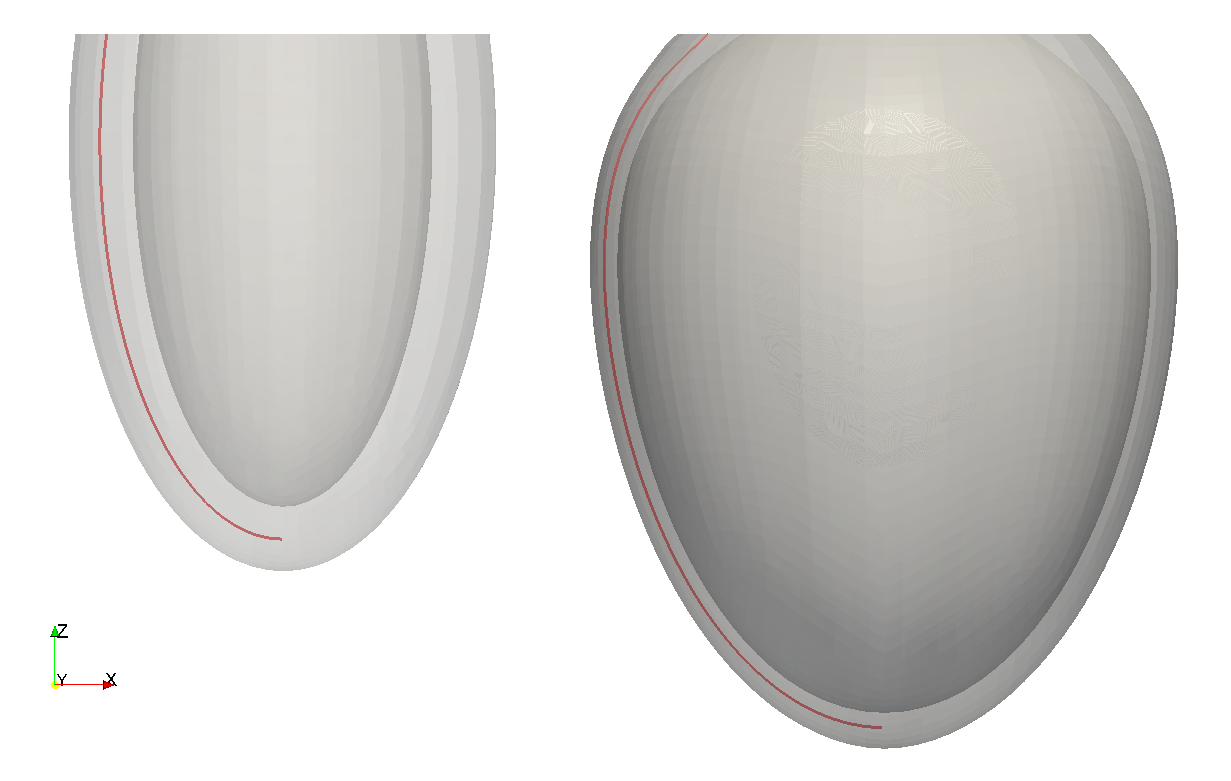
\includegraphics[scale=0.18]{media/5-verif/5-land2/land2-2.png}
\label{fig:ventricles2}}		
\subfigure[]{%
		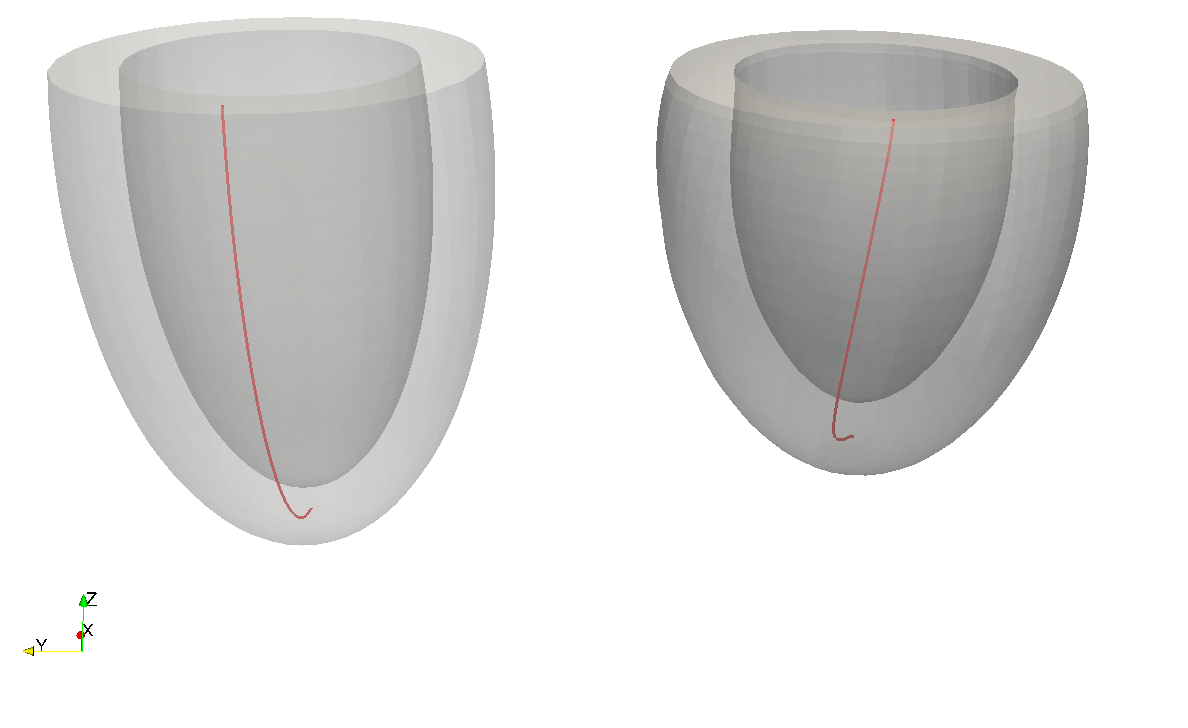
\includegraphics[scale=0.18]{media/5-verif/6-land3/land3-1.png}
\label{fig:ventricles3}}		
\subfigure[]{%
		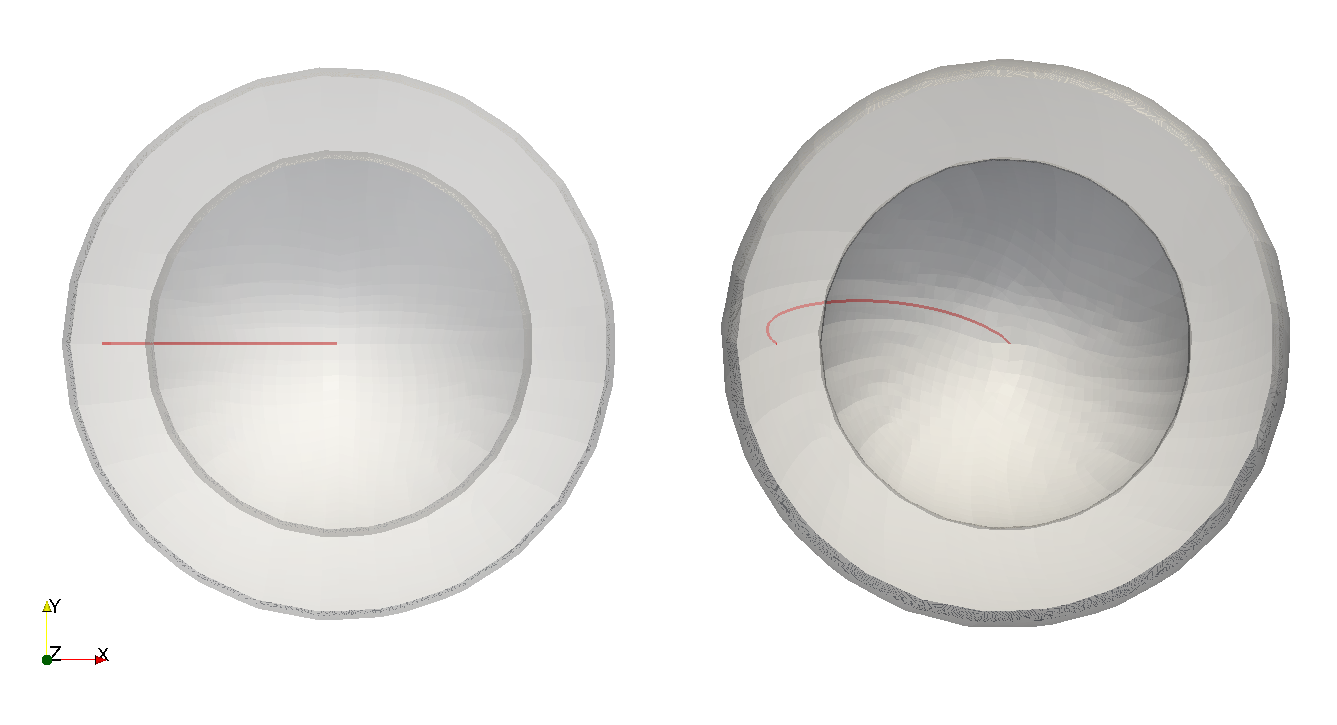
\includegraphics[scale=0.16]{media/5-verif/6-land3/land3-2.png}
\label{fig:ventricles4}}		
%
\caption{Undeformed (left) and deformed (right) configurations for single ventricle verification problems: (a,b) Land P2: inflation, and (c,d) Land P3: inflation and active contraction. The red curve denotes the curve over which displacements and positions are recorded and compared.}
\label{fig:ventricles}
\end{figure}

Figures \ref*{fig:gurev2}-\ref*{fig:land3.2} show the results for the six verification problems, mimicking the format used in the papers from which they came. The results presented compare Cardioid, Celeris, and an in-house conventional finite element code \textit{Imitor}. The implementation considerations are nearly identical for Imitor and Celeris, which allows us to distinguish between differences related to the finite element formulation and differences related to how incompressibility was enforced.

For the cantilever beam problems Gurev P2, Gurev P3, Gurev P4, and Land P1, a 39 $\times$ 4 $\times$ 4 hex mesh is used. In the case of Cardioid and Imitor, linear hexahedral elements are employed. For the case of Celeris, linear cuboidal PEM elements are used. Thus, the element shapes are the same, but the element formulations differ. The polyhedral code Celeris performs very well in bending, torsion, and active contraction - the deformed meshes nearly identically match for all three codes.

For the single ventricle problems Land P2 and Land P3, quadratic tetrahedral elements are used in Cardioid and linear hexahedral elements are used in Imitor. An adequate number of degrees of freedom were used to achieve converged results. A polyhedral mesh was generated for the problems but has not yet been tested, pending some fixes in the Celeris infrastructure unrelated to the scope of this project. The results for the single ventricle problems are satisfactorily close between Imitor and Cardioid, despite the difference in element choice and enforcement of incompressibility, which is promising since the material model implementation is nearly identical between Imitor and Celeris.

Interestingly, Imitor's results appear to be slightly too stiff in bending, but slightly too compliant for volumetric deformations. The over-stiffness in bending is evidenced in Gurev P2, Land P1, and Land P2, whereas the over-compliance in volumetric deformation is evidenced in Gurev P4 and Land P3. More investigation would be required to attribute this difference to the enforcement near-incompressibility rather than a fully incompressible material. Overall though, the difference in results is small enough to provide confidence that the material model has been implemented correctly in Imitor and in Celeris.

A comparison of the number of degrees of freedom for the three codes in the bending problem Land P1 is provided (\figref{land1-3}). It was not expected to be useful because the meshes are already quite coarse, and automated linear hex meshing for a simple cantilever beam geometry is easily achievable. It is expected that for the single ventricle problems Land P2 and Land P3, accurate results can be achieved using Celeris with a noticeable reduction in the number of DOF, which would complete \figref{land2-3} and \figref{land3.2-3}.

Up to this point, the mechanics implemented in Imitor and Celeris have been verified, and cuboidal polyhedral elements are performing well for the cantilever beam problems. Completing the verification process would involve running Land P2 and Land P3 in Celeris with general polyhedral elements, as well as potentially running the cantilever beam problems again in Celeris with non-cuboidal polyhedral elements. Once the fixes in Celeris are made, the suite of verification problems can be completed, after which point the code would be ready to perform the same cardiac simulations presented using Cardioid.

\begin{figure}[ht]
\centering
\subfigure[]{%
		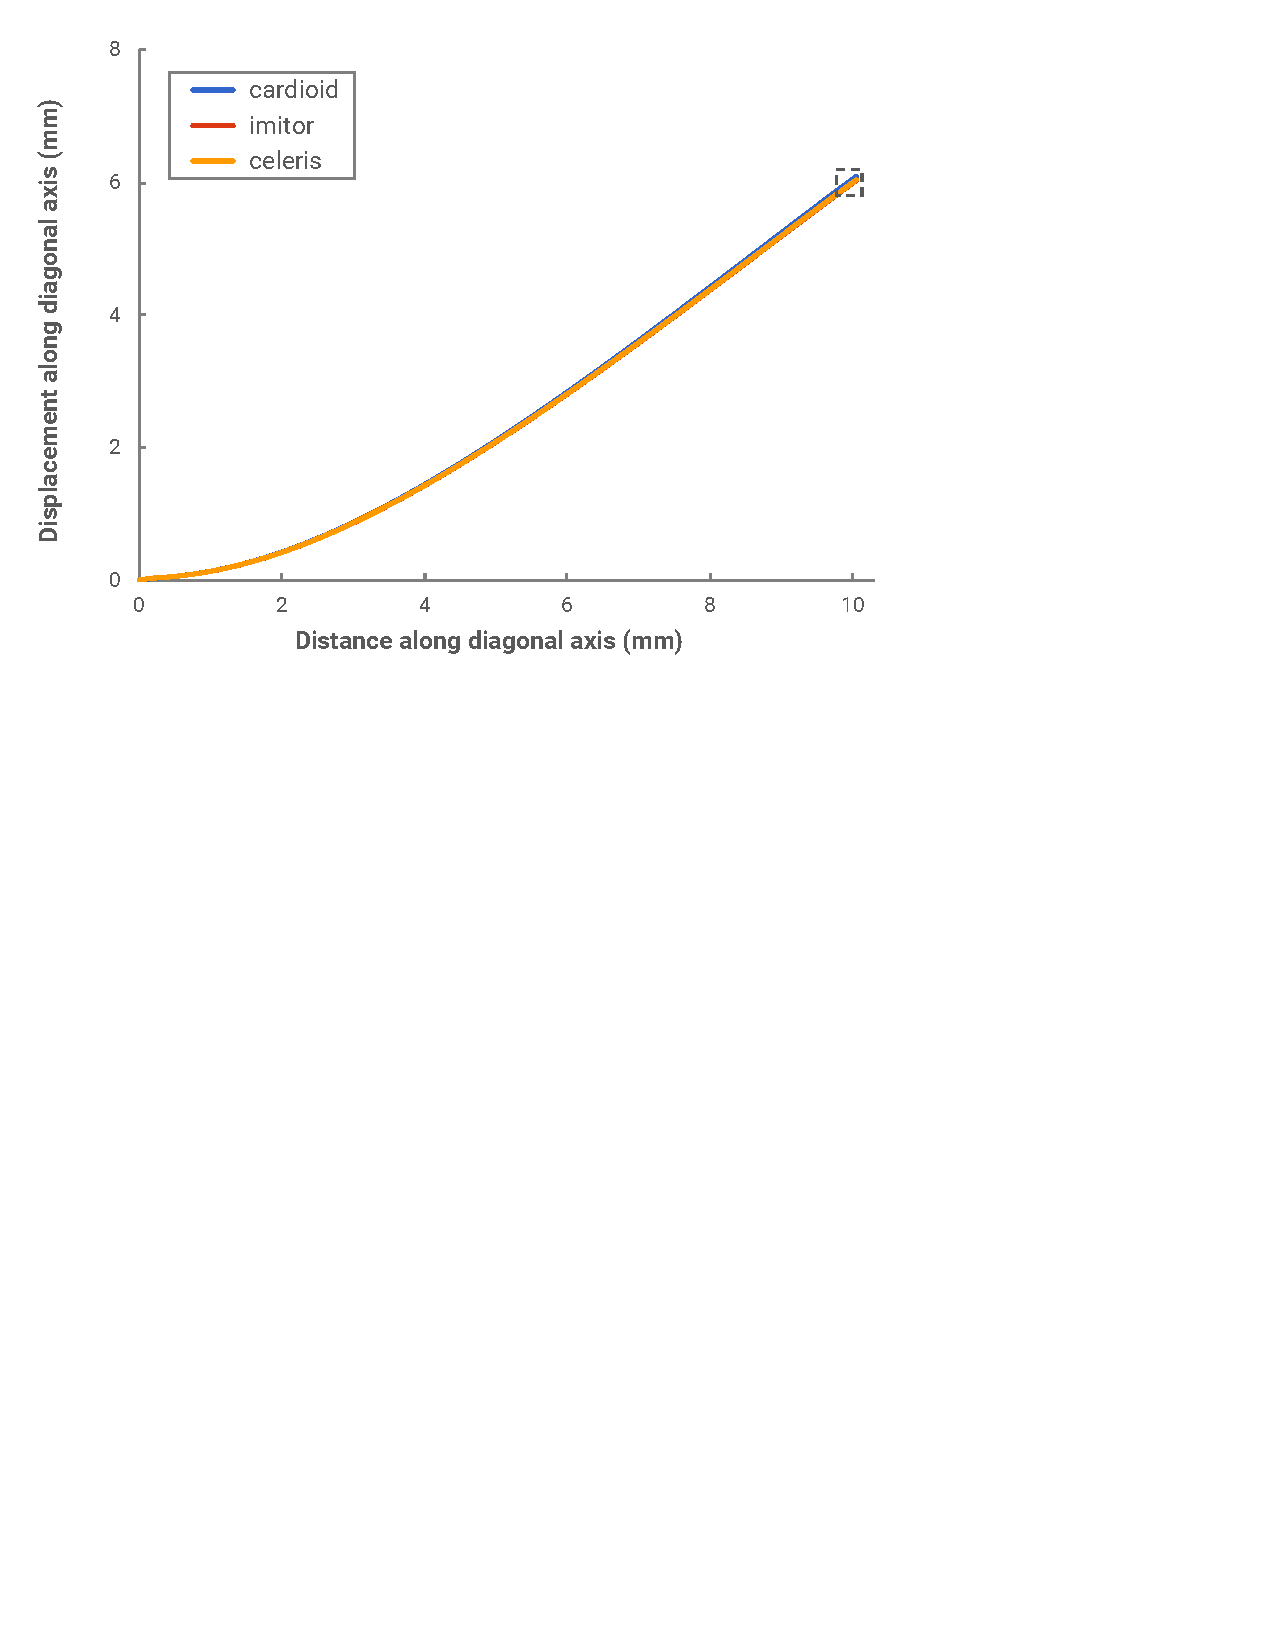
\includegraphics[scale=0.46]{media/5-verif/1-gurev2/gurev2-1.pdf}
\label{fig:gurev2-1}}		
\subfigure[]{%
		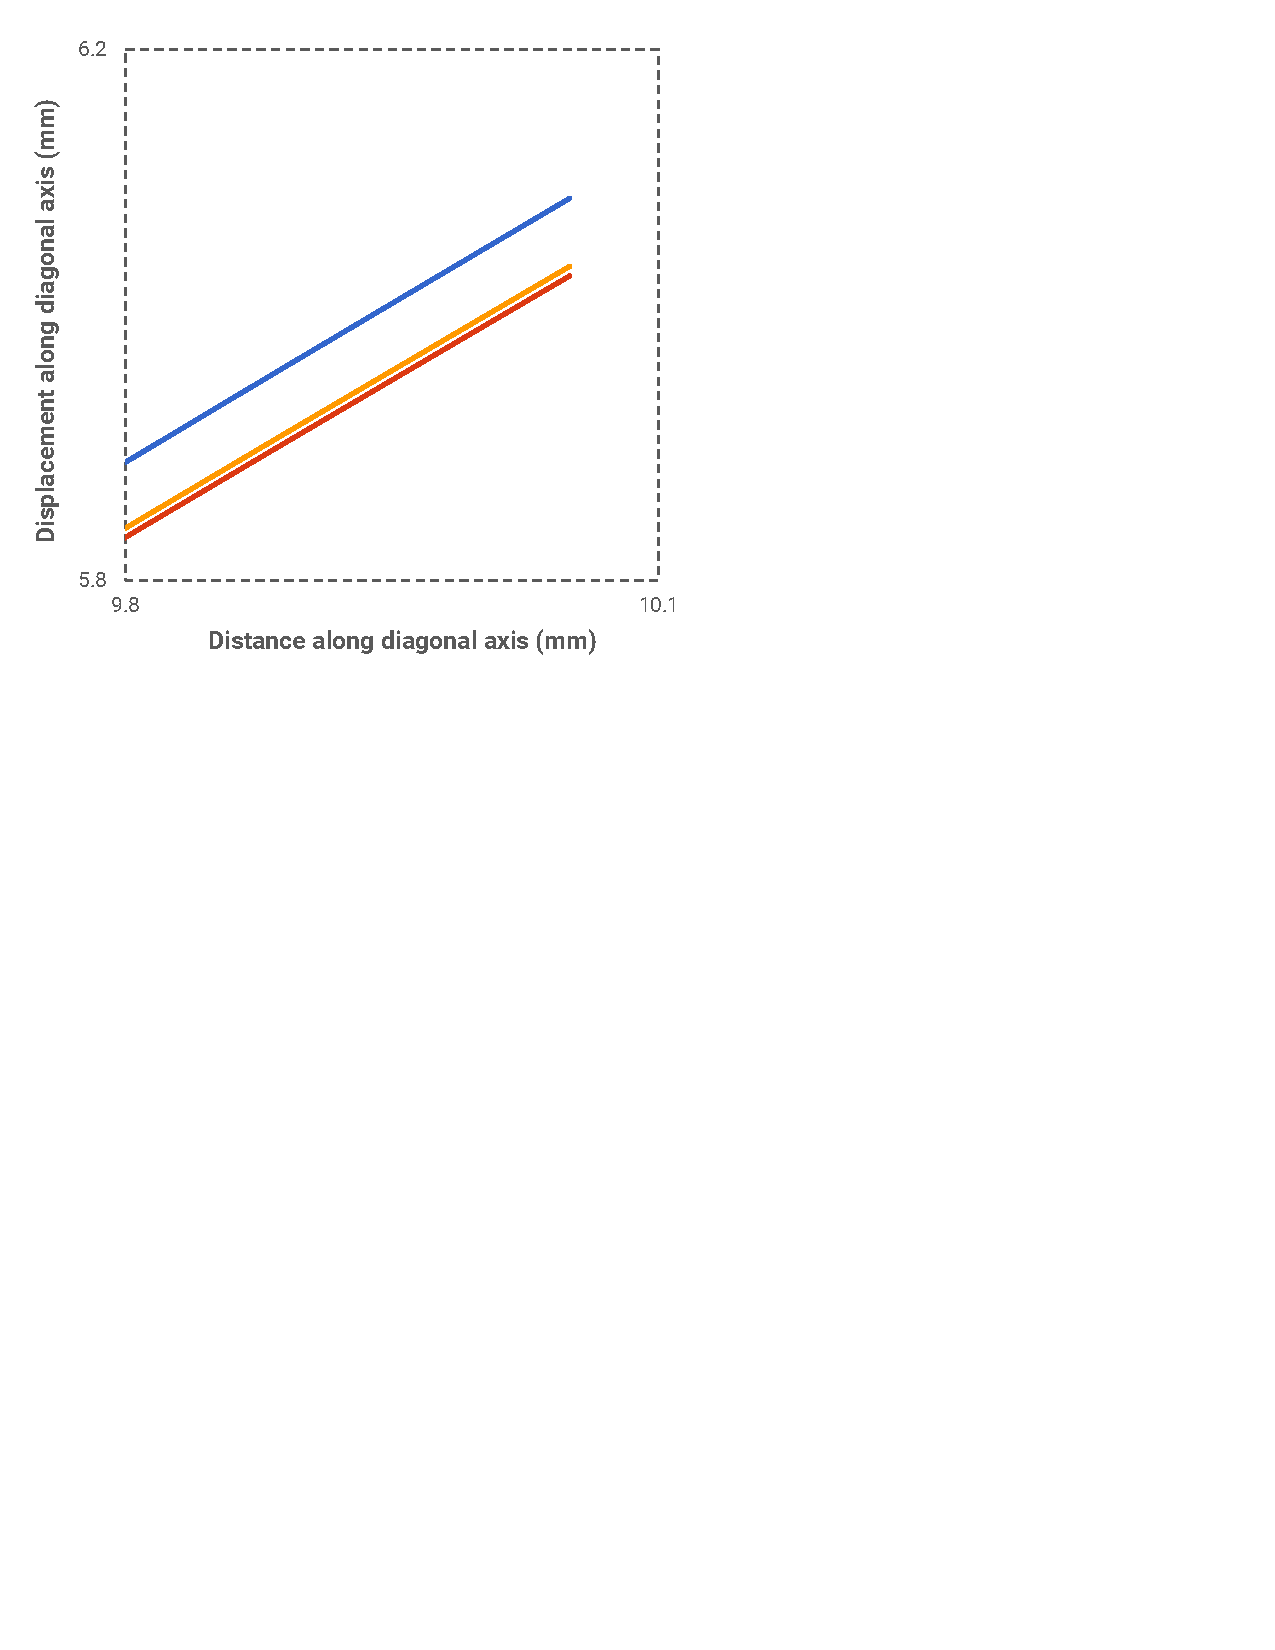
\includegraphics[scale=0.46]{media/5-verif/1-gurev2/gurev2-2.pdf}
\label{fig:gurev2-2}}		
%
\caption{Results for Gurev P2 verification problem: (a) Displacement magnitude along diagonal axis, with (b) details for the free end of the beam}
\label{fig:gurev2}
\end{figure}

\begin{figure}[ht!]
\centering
\subfigure[]{%
		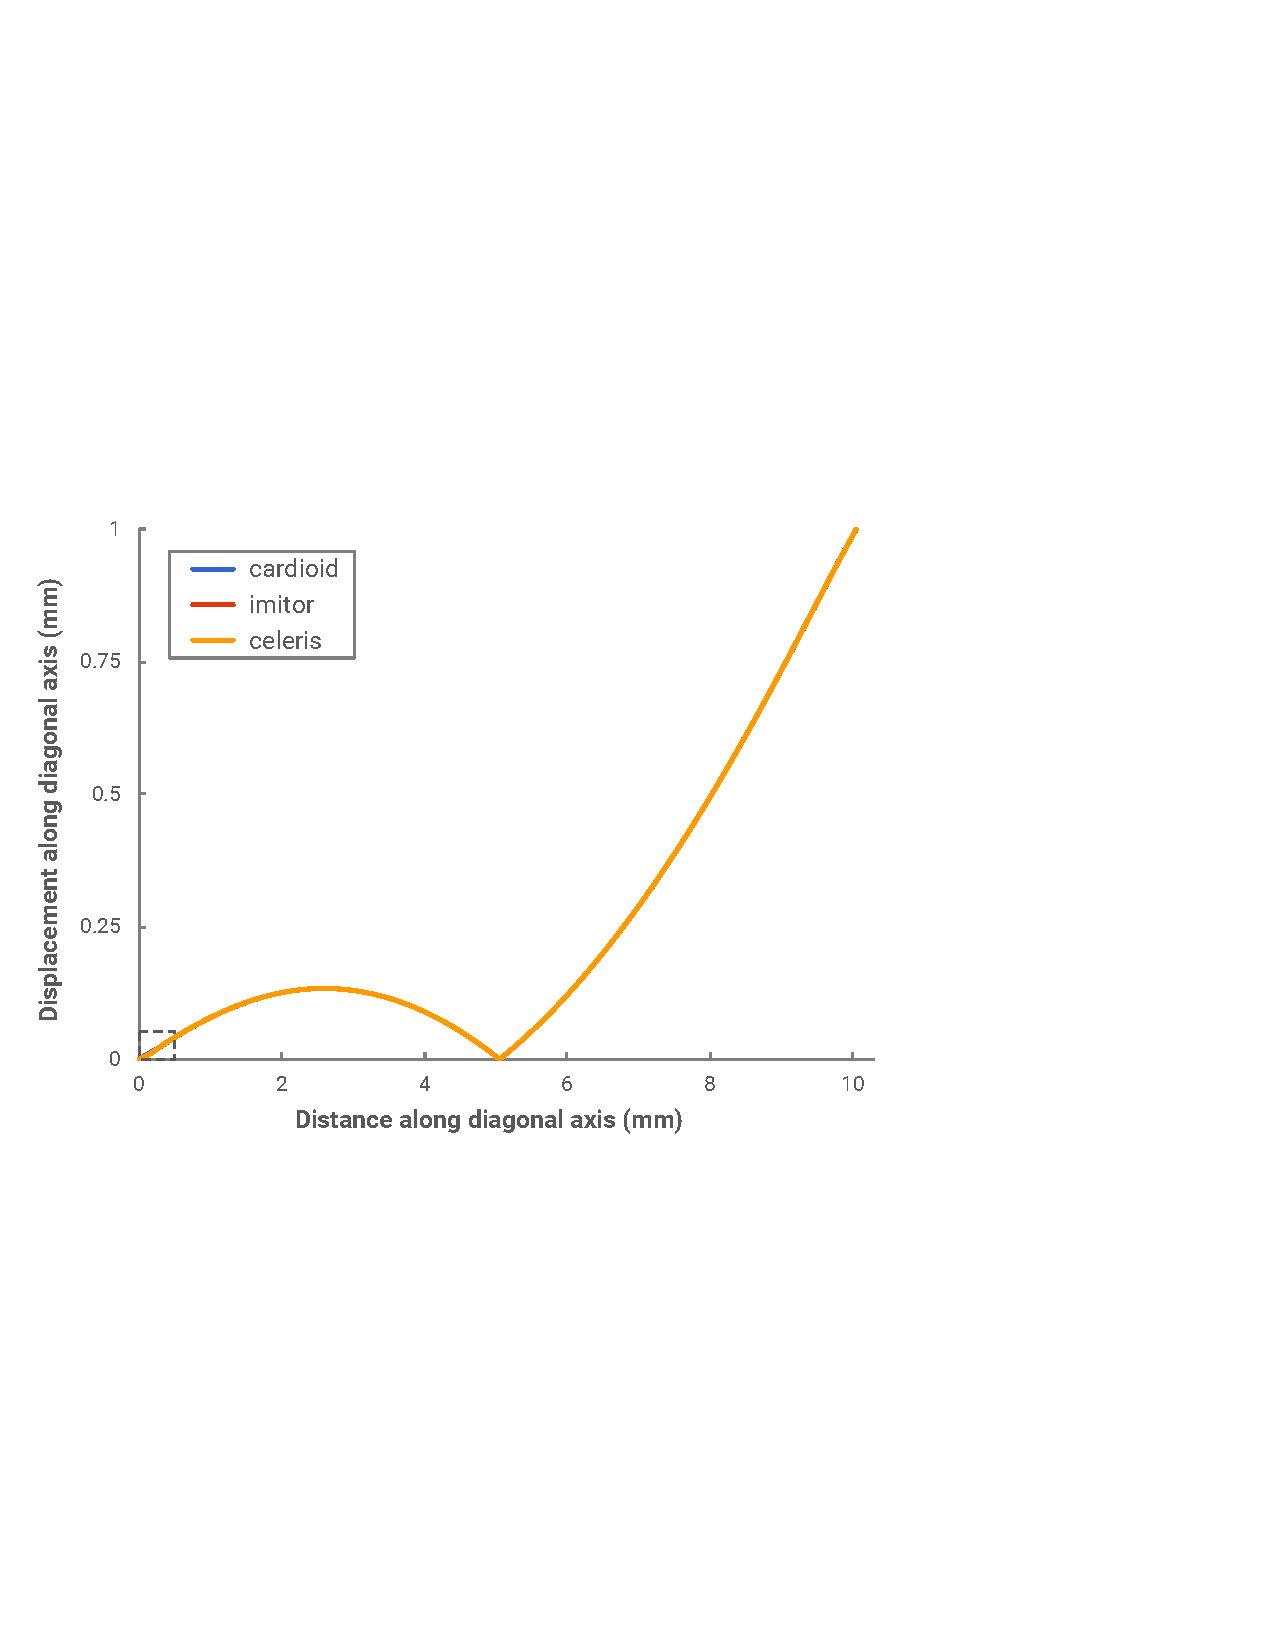
\includegraphics[scale=0.46]{media/5-verif/2-gurev3/gurev3-1.pdf}
\label{fig:gurev3-1}}		
\subfigure[]{%
		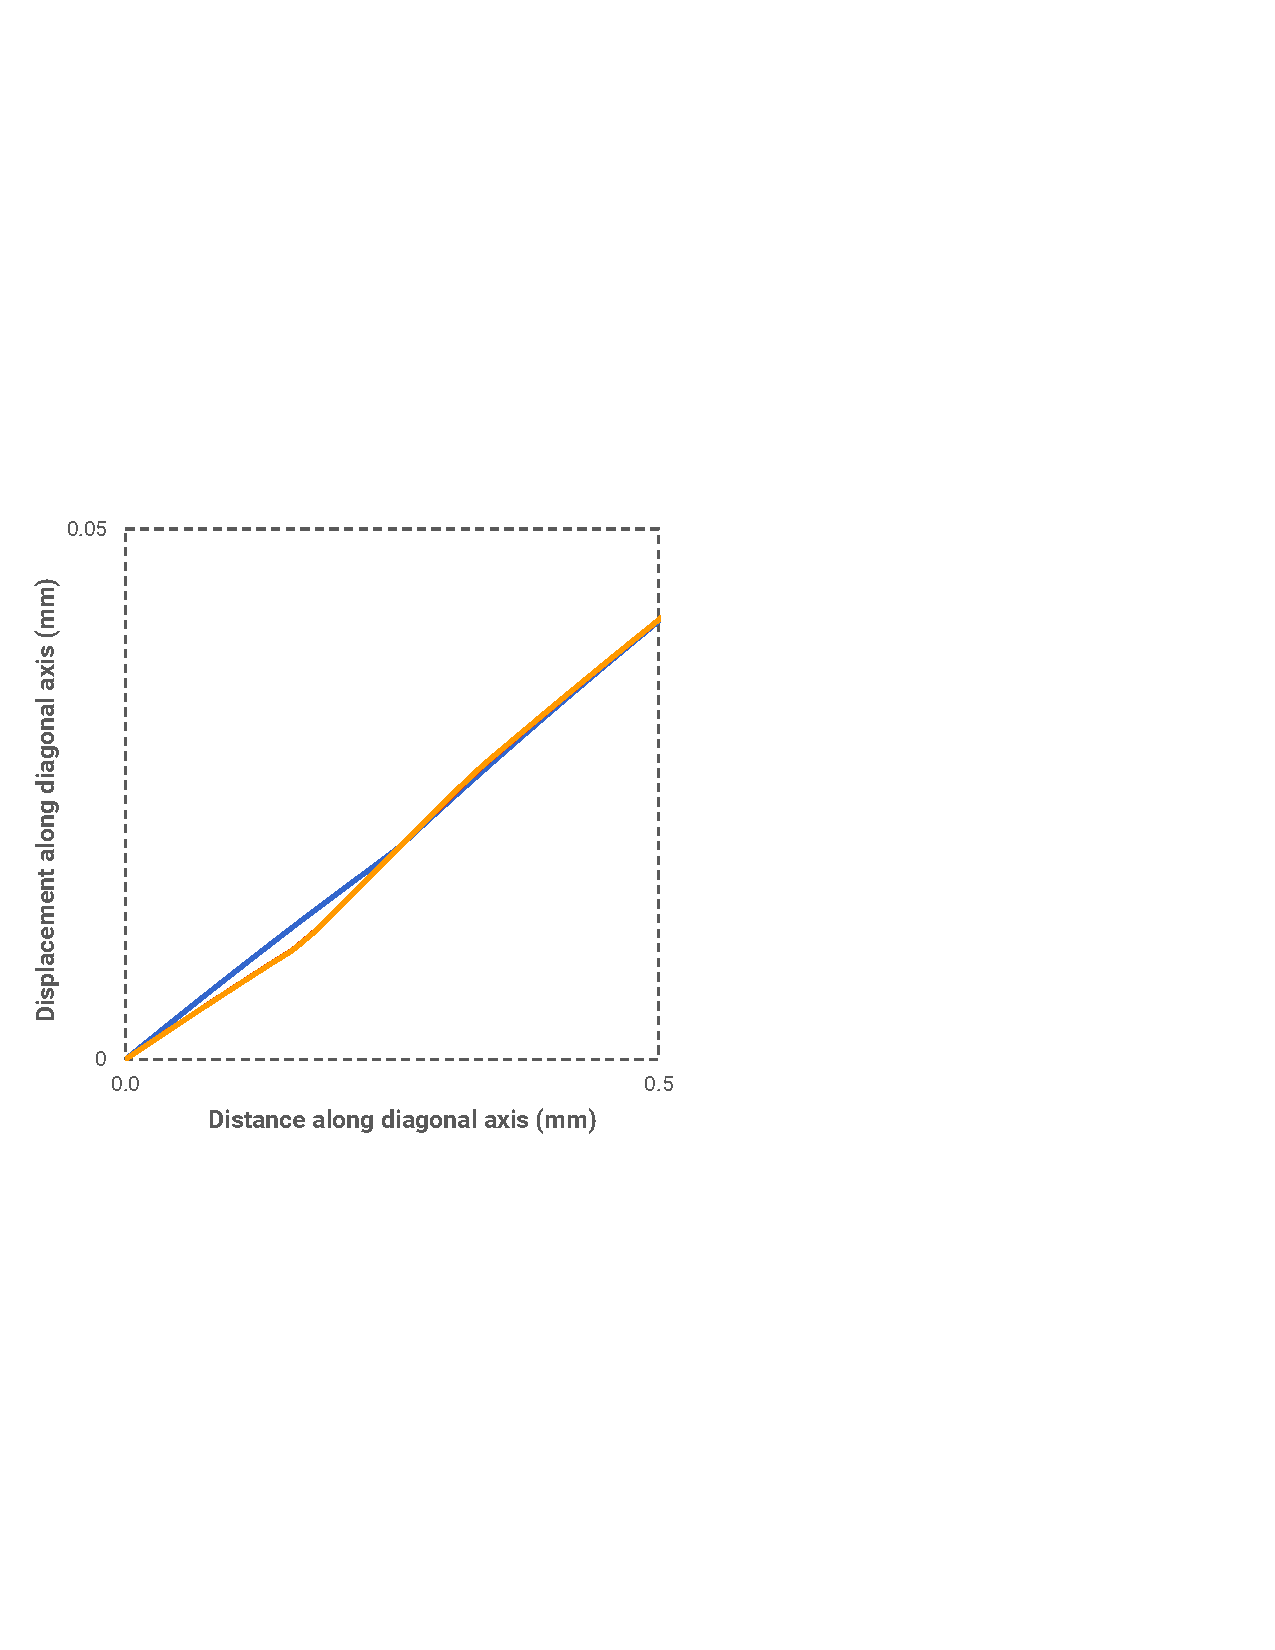
\includegraphics[scale=0.46]{media/5-verif/2-gurev3/gurev3-2.pdf}
\label{fig:gure3-2}}		
%
\caption{Results for Gurev P3 verification problem: (a) Displacement magnitude along diagonal axis, with (b) details for the fixed end of the beam. The results for Imitor and Celeris are indistinguishable in these plots.}
\label{fig:gurev3}
\end{figure}

\begin{figure}[ht!]
\centering
\subfigure[]{%
		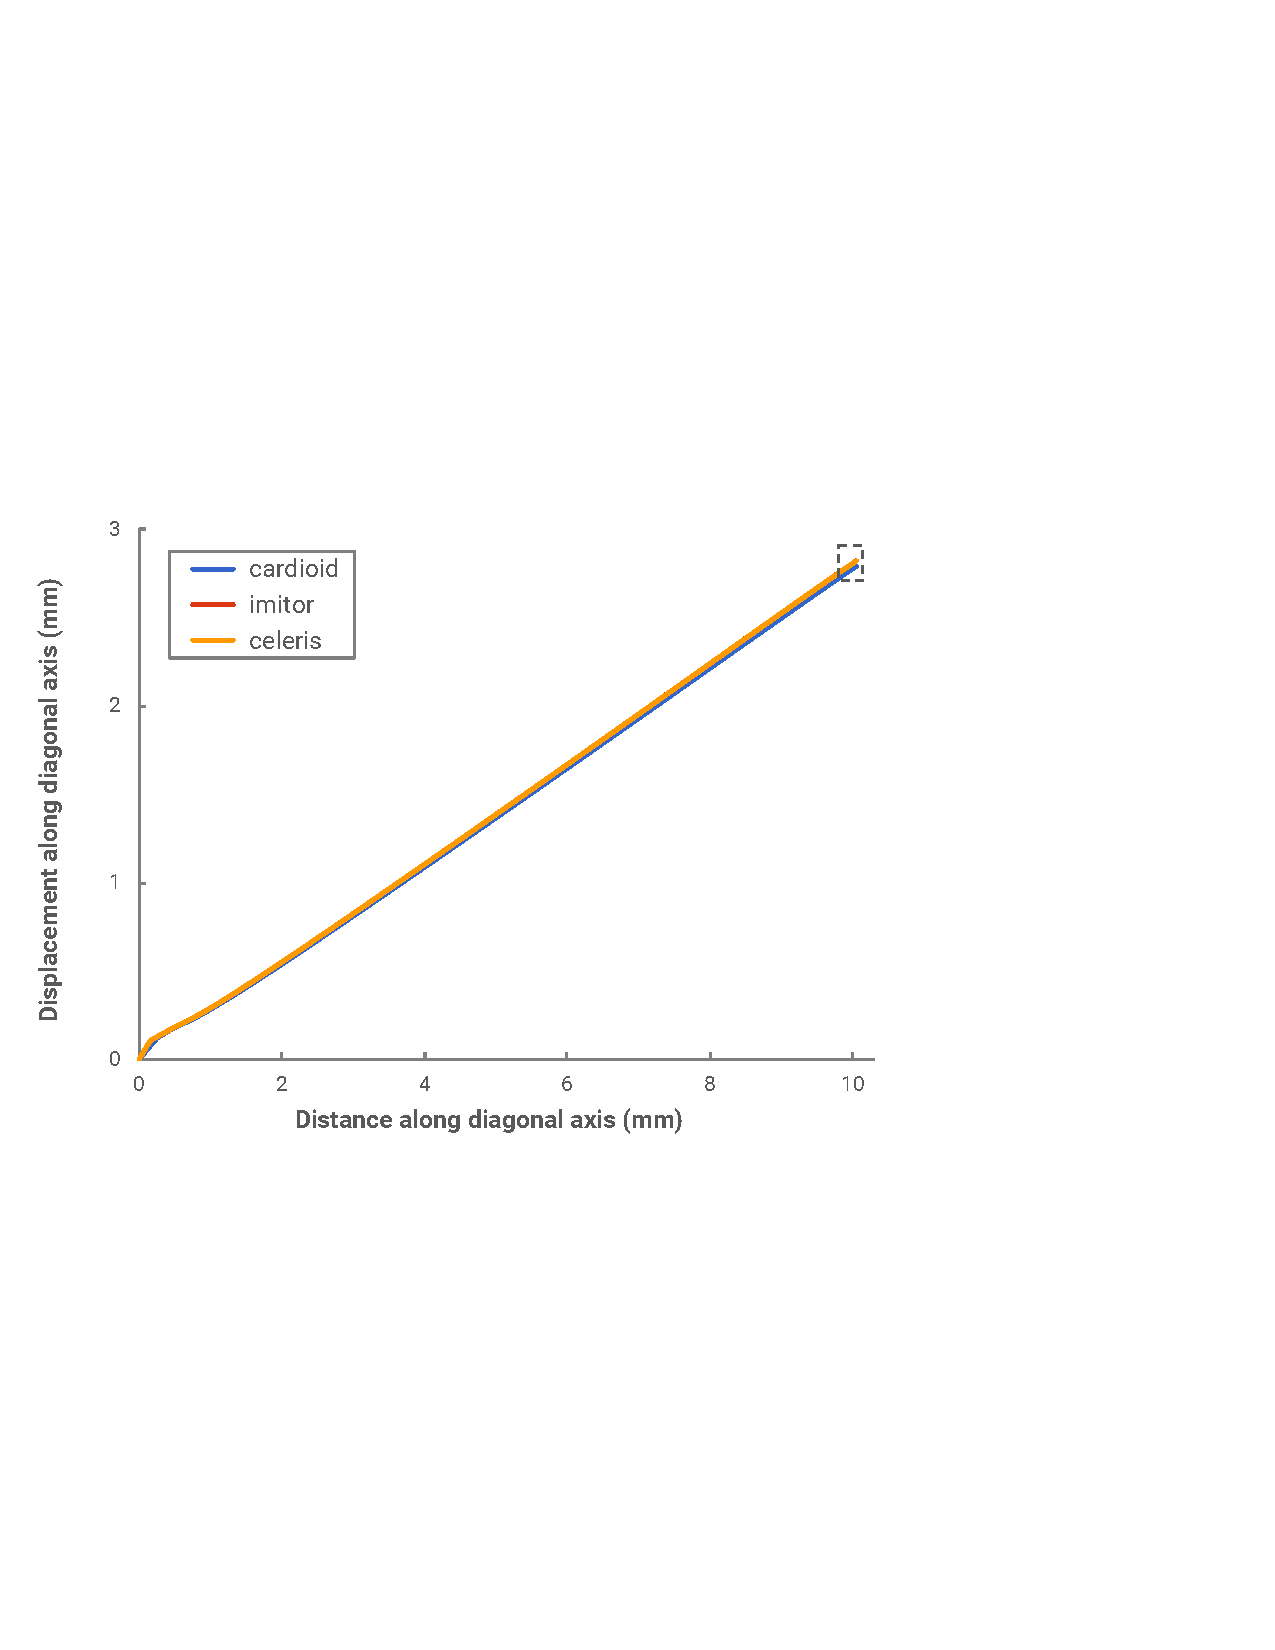
\includegraphics[scale=0.46]{media/5-verif/3-gurev4/gurev4-1.pdf}
\label{fig:gurev4-1}}		
\subfigure[]{%
		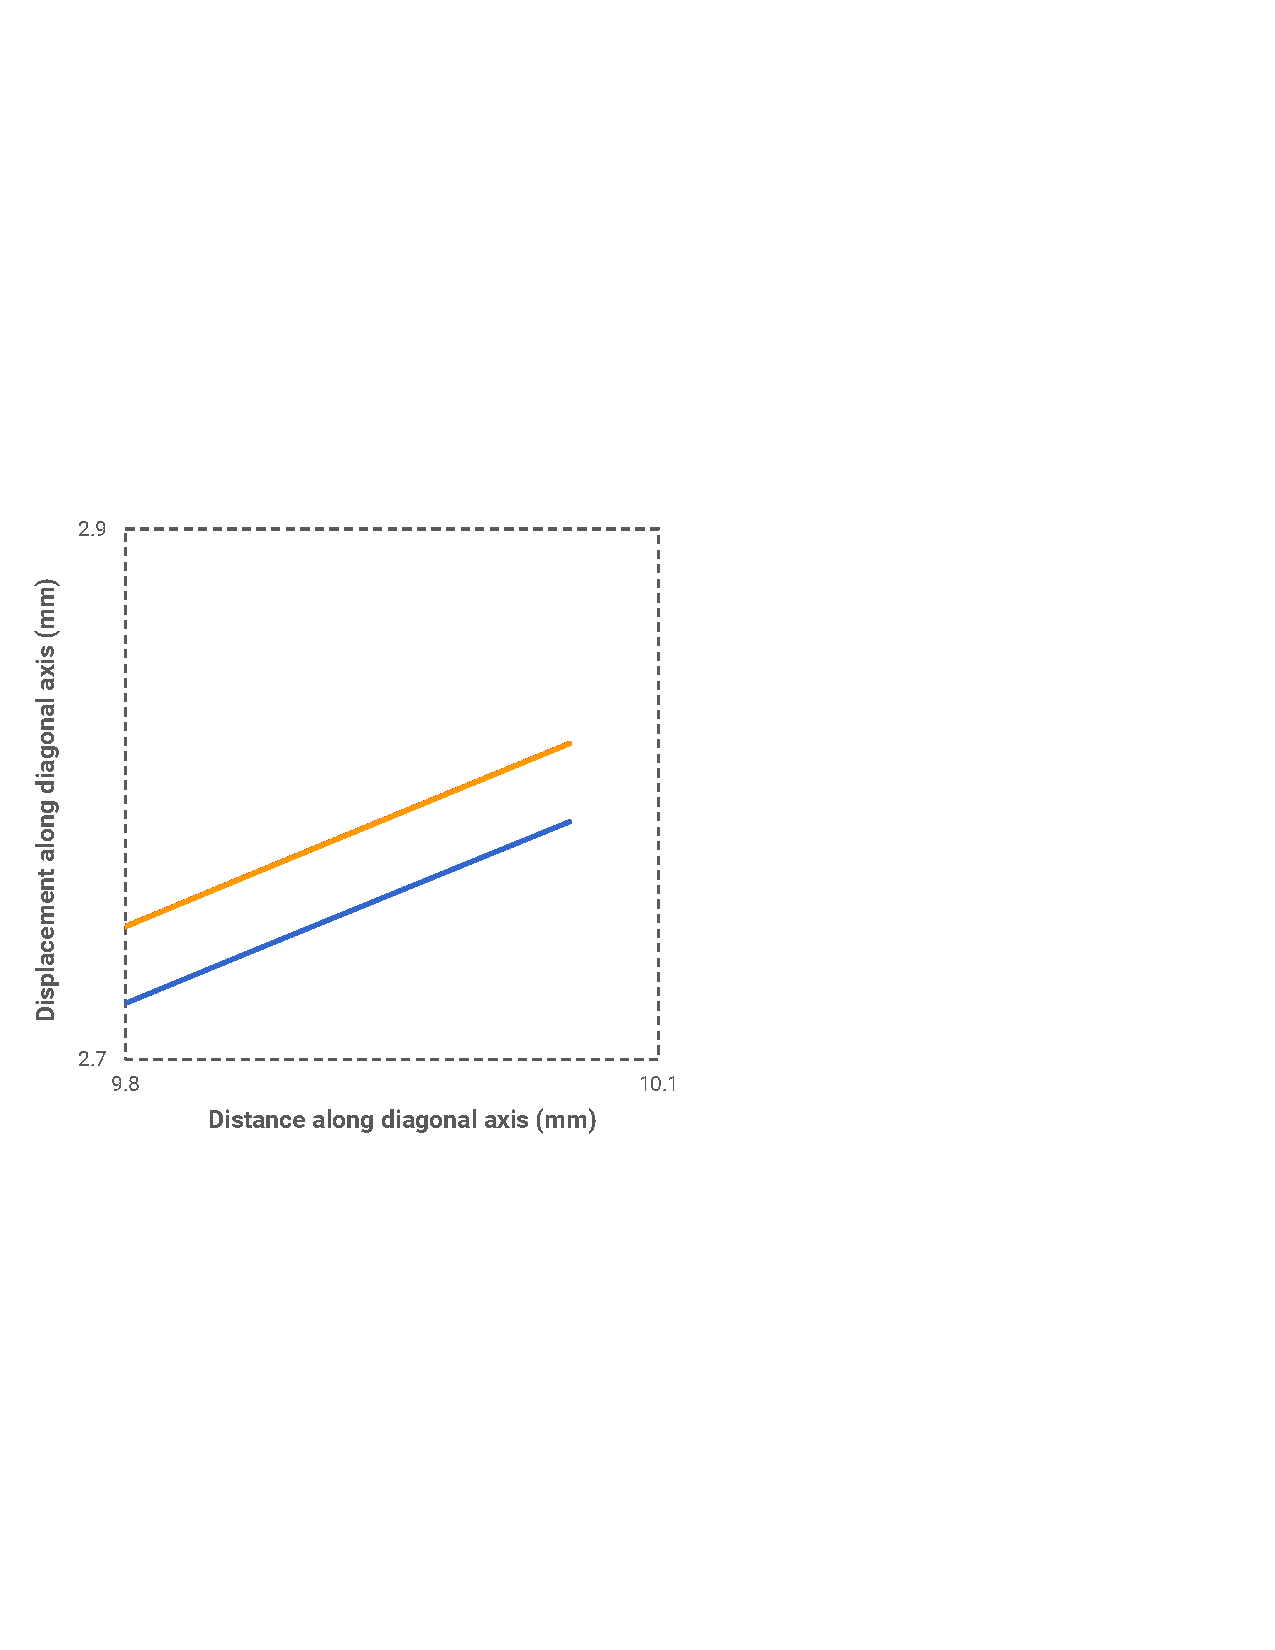
\includegraphics[scale=0.46]{media/5-verif/3-gurev4/gurev4-2.pdf}
\label{fig:gurev4-2}}		
%
\caption{Results for Gurev P4 verification problem: (a) Displacement magnitude along diagonal axis, with (b) details for the free end of the beam. The results for Imitor and Celeris are indistinguishable in these plots.}
\label{fig:gurev4}
\end{figure}

\begin{figure}[ht!]
\centering
\subfigure[]{%
		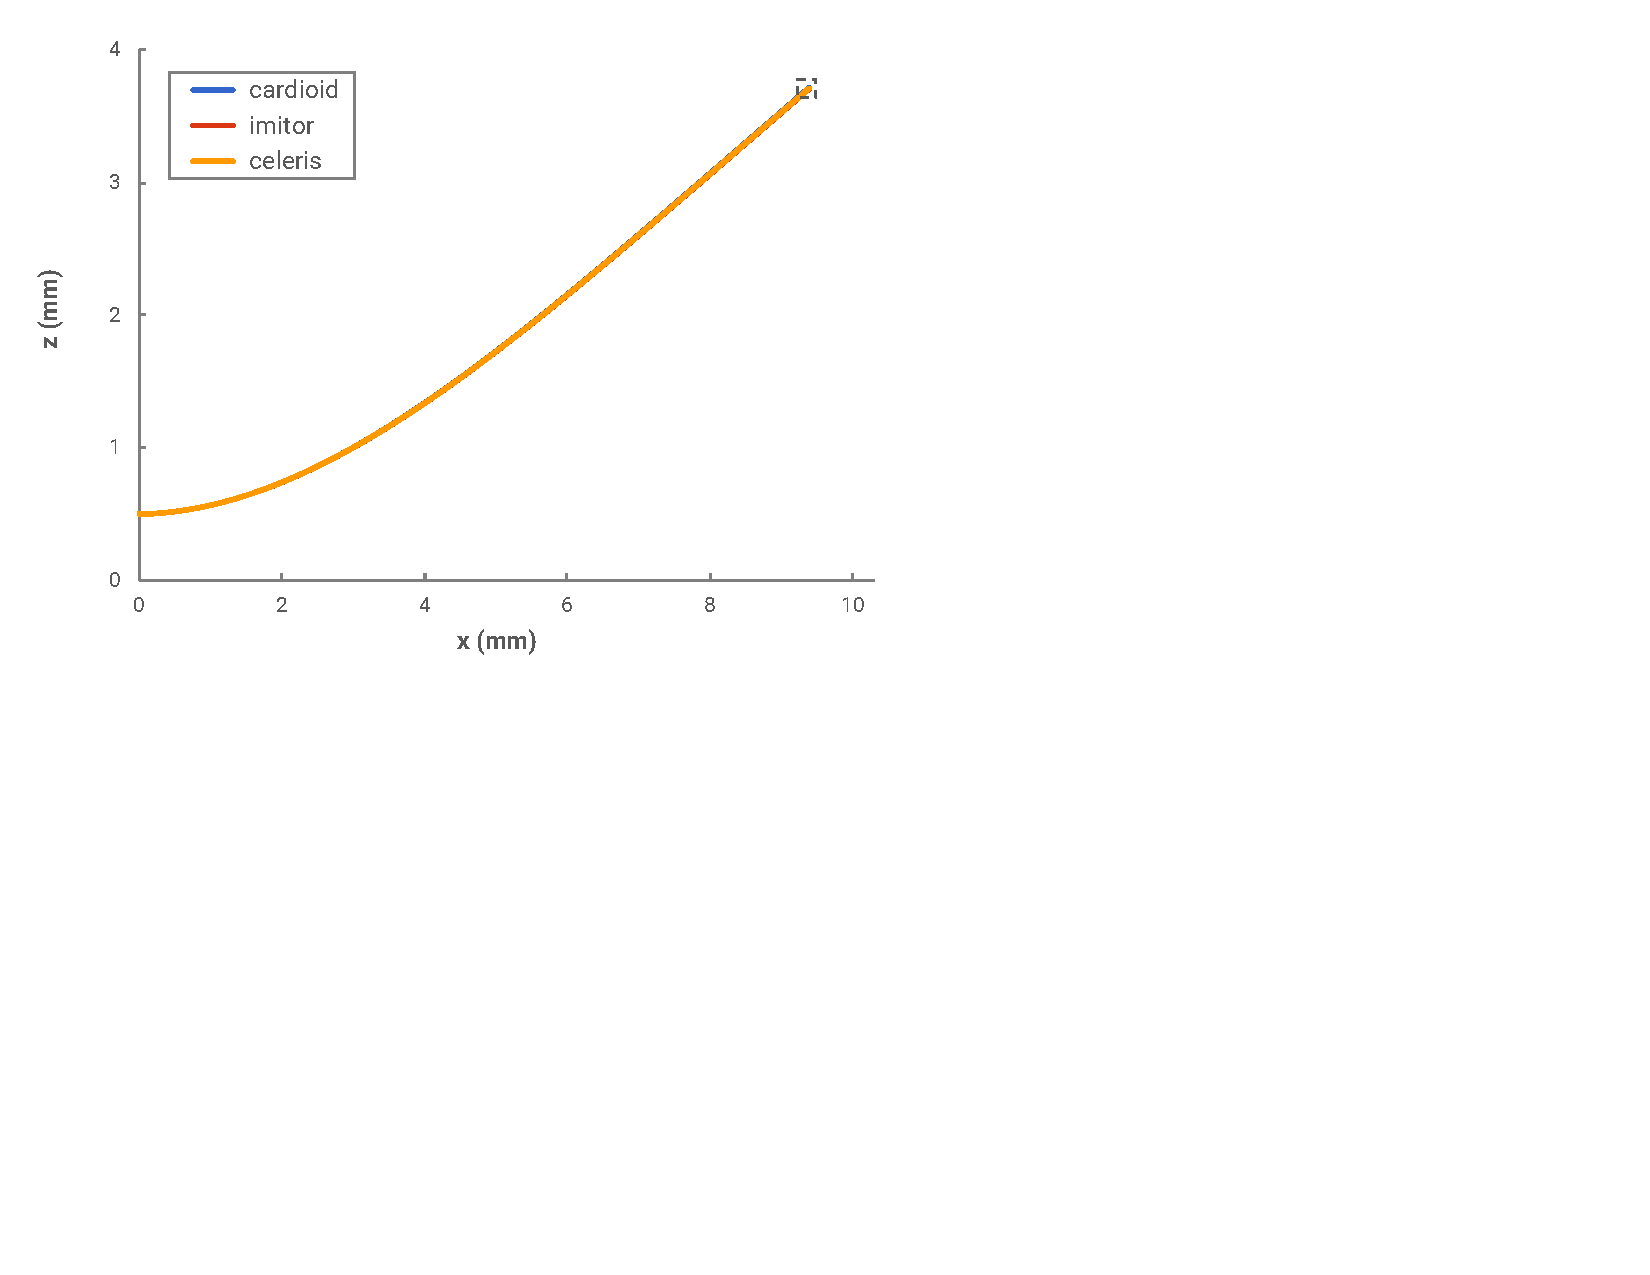
\includegraphics[scale=0.46]{media/5-verif/4-land1/land1-1.pdf}
\label{fig:land1-1}}		
\subfigure[]{%
		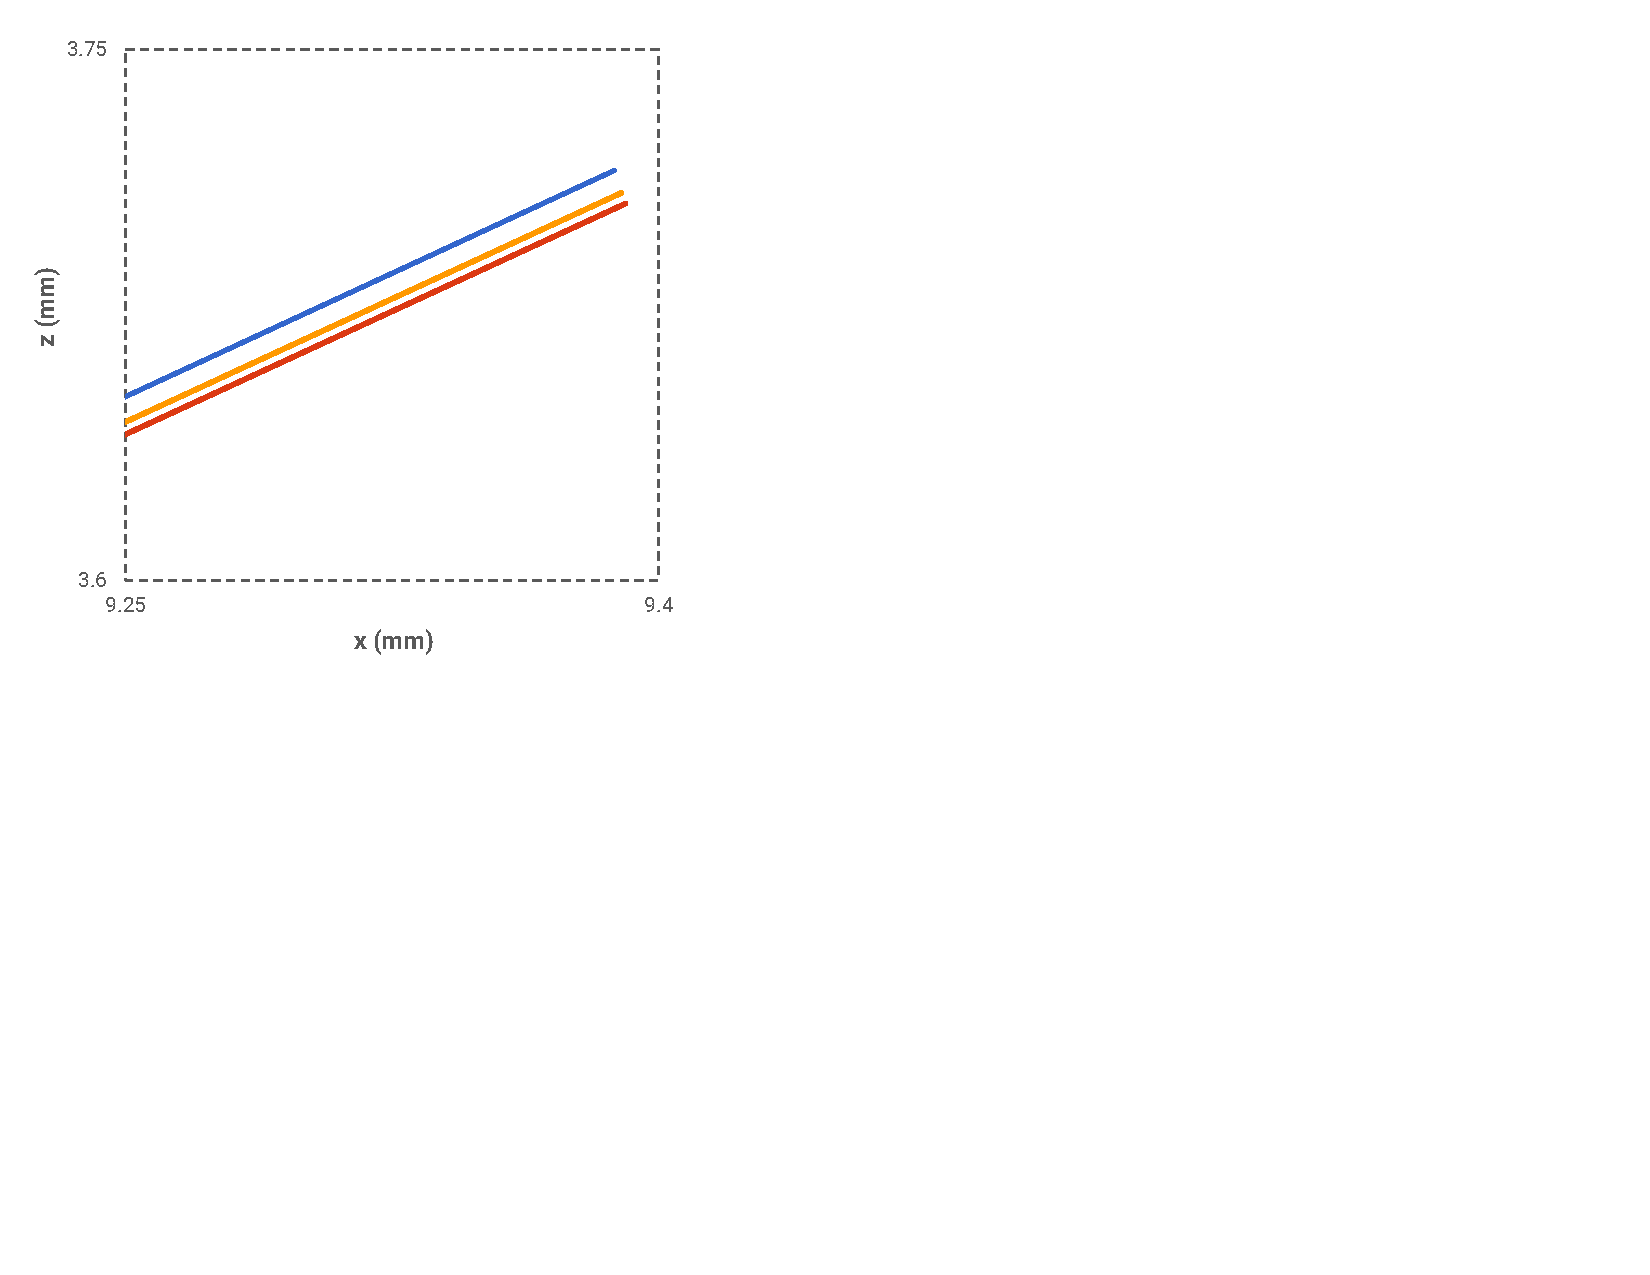
\includegraphics[scale=0.46]{media/5-verif/4-land1/land1-2.pdf}
\label{fig:land1-2}}	
\subfigure[]{%
		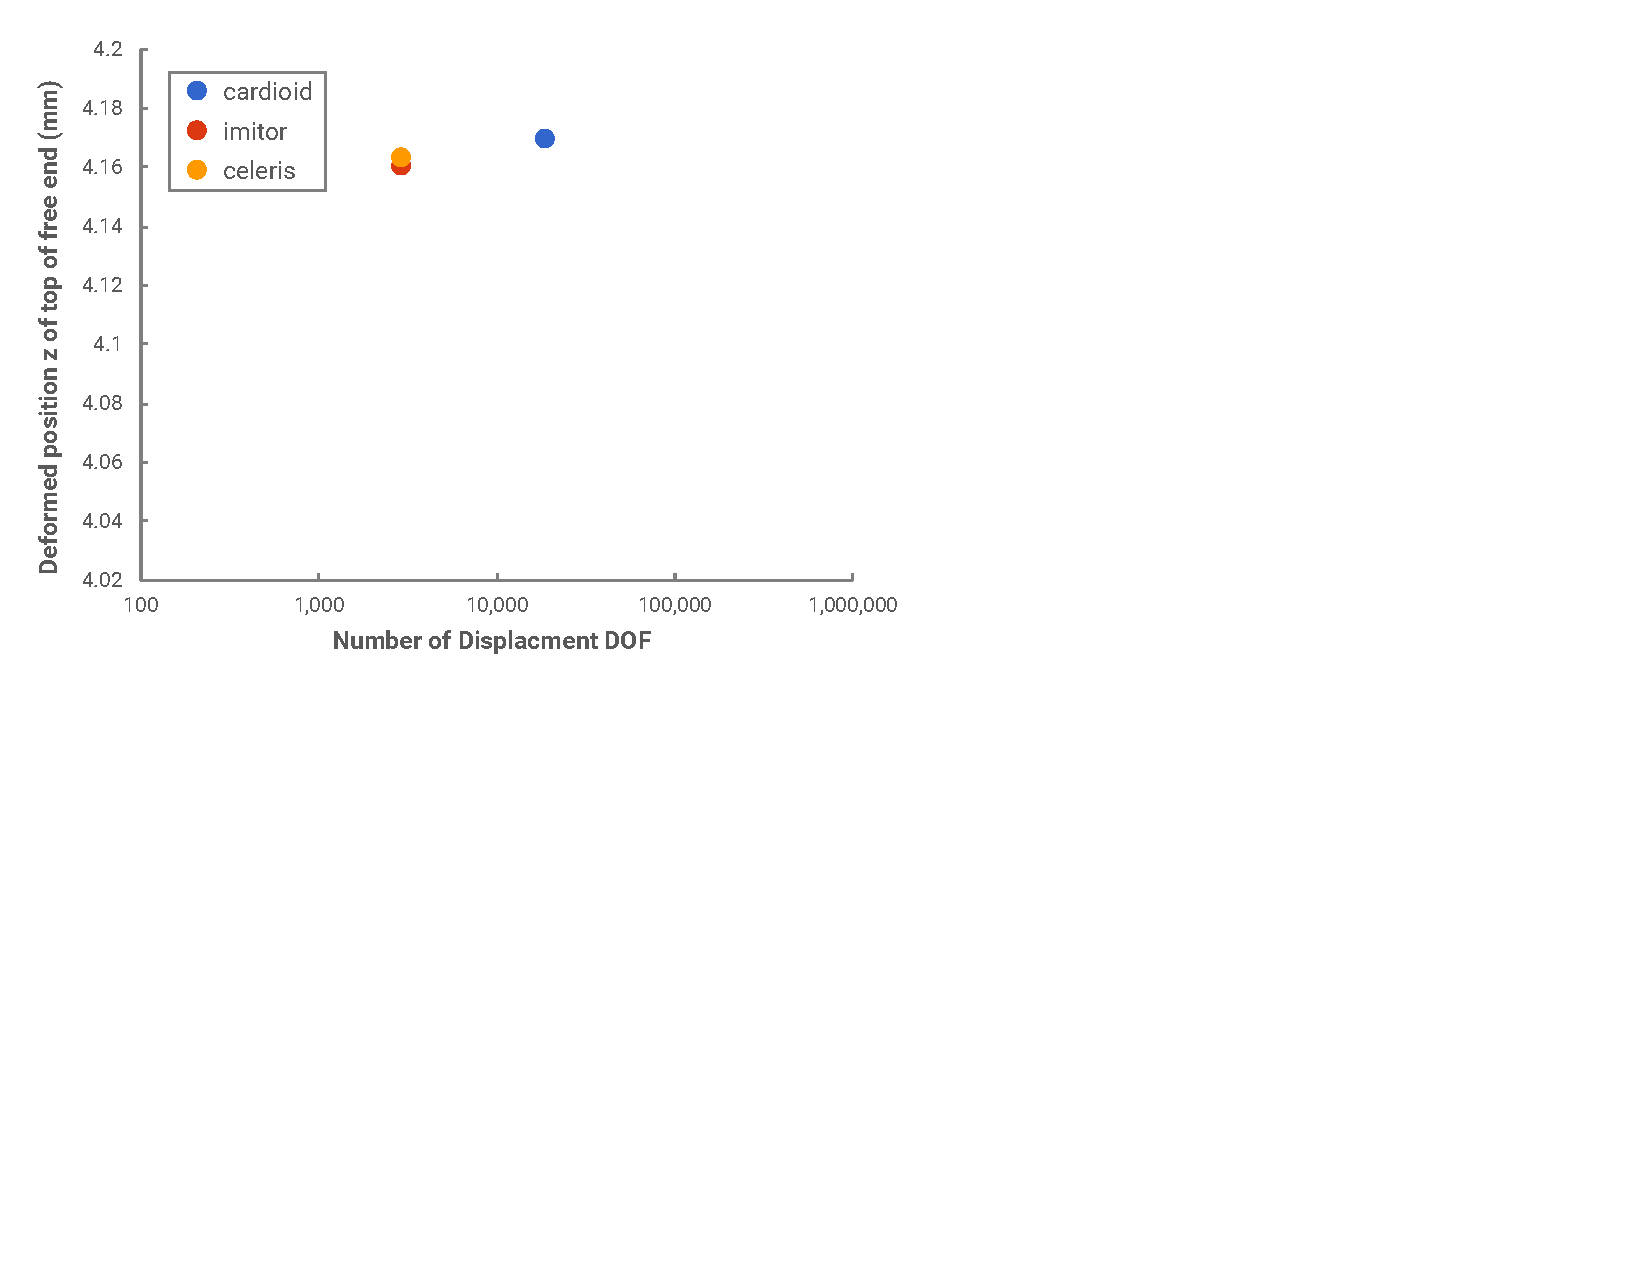
\includegraphics[scale=0.46]{media/5-verif/4-land1/land1-3.pdf}
\label{fig:land1-3}}			
%
\caption{Results for Land P1 verification problem: (a) Deformed position of midline, with (b) details for the free end of the beam. Panel (c) shows the deformed position of the point $\bm{X} = (10, 0.5, 1)$ for each of the simulation codes.}
\label{fig:land1}
\end{figure}


\begin{figure}[ht!]
\centering
\subfigure[]{%
		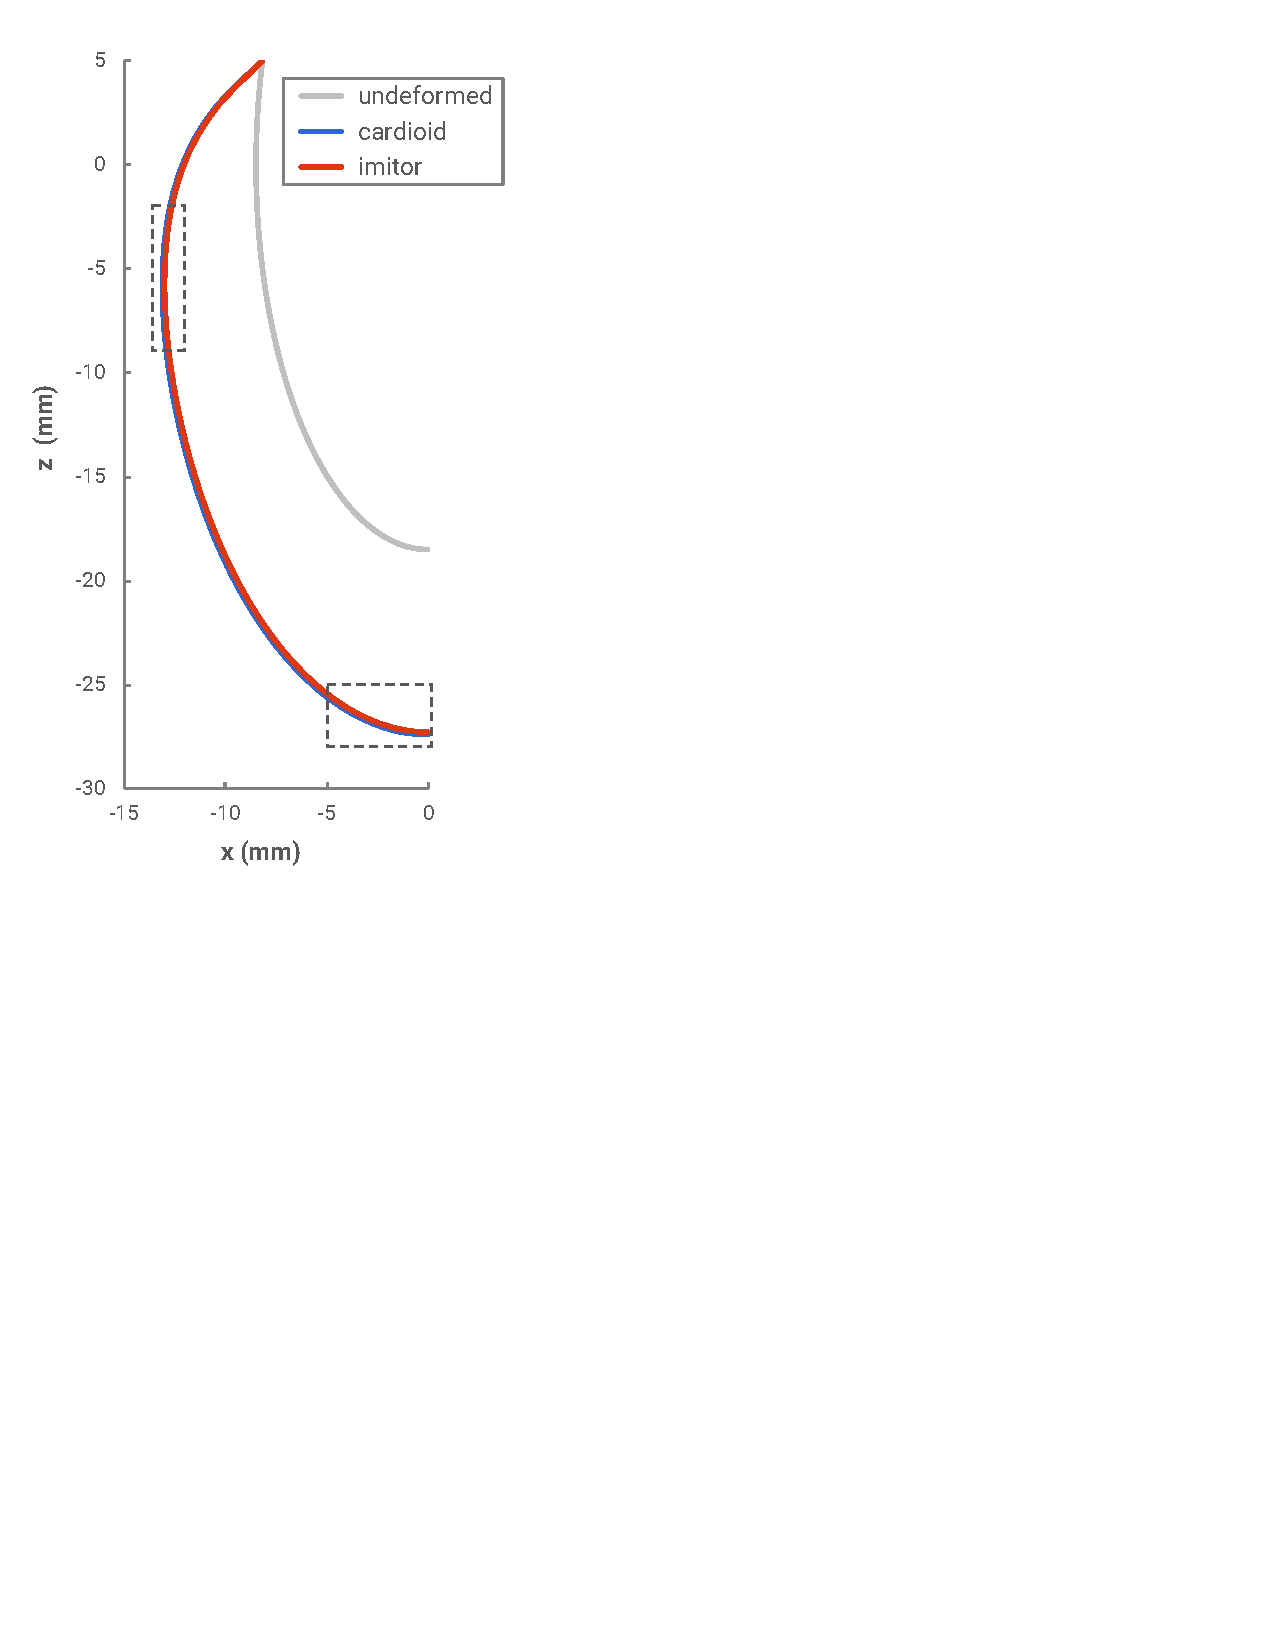
\includegraphics[scale=0.46]{media/5-verif/5-land2/land2-1.pdf}
\label{fig:land2-1}}		
\subfigure[]{%
		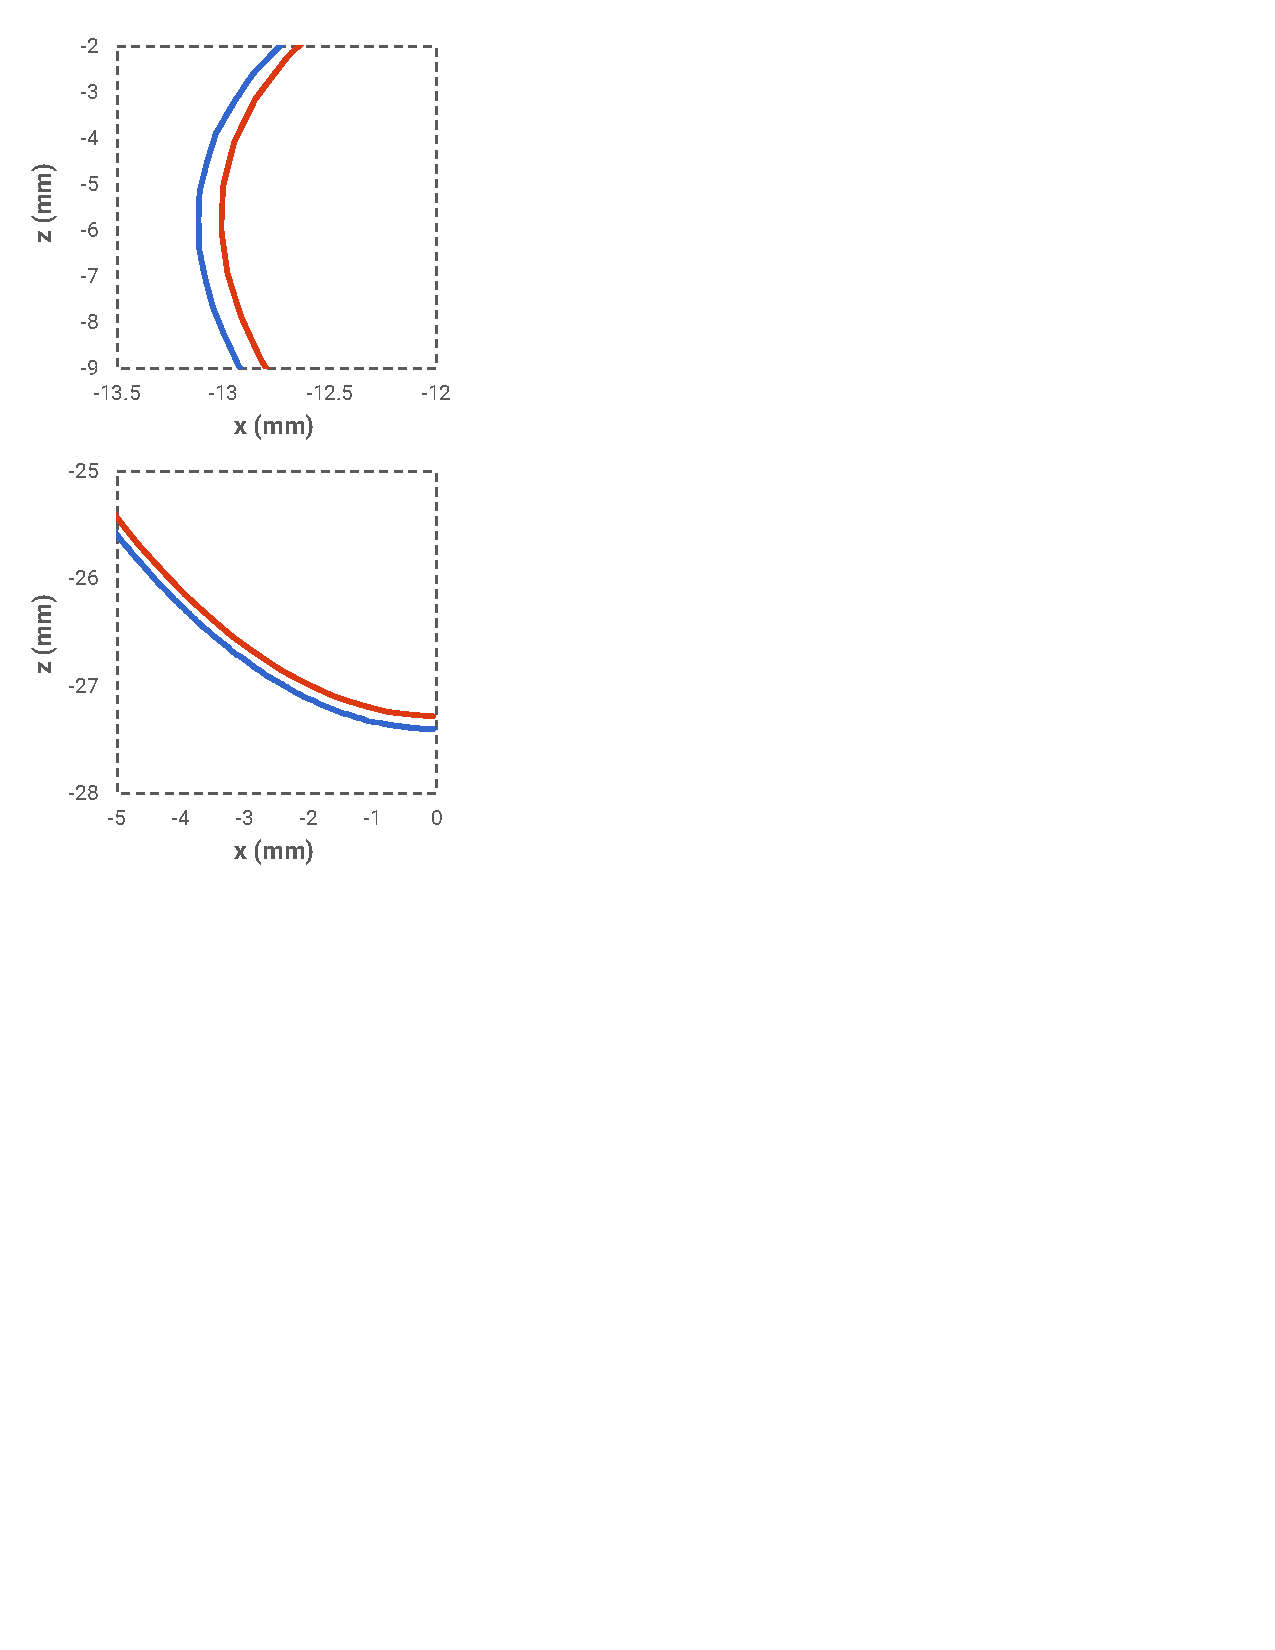
\includegraphics[scale=0.46]{media/5-verif/5-land2/land2-2.pdf}
\label{fig:land2-2}}	
\subfigure[]{%
		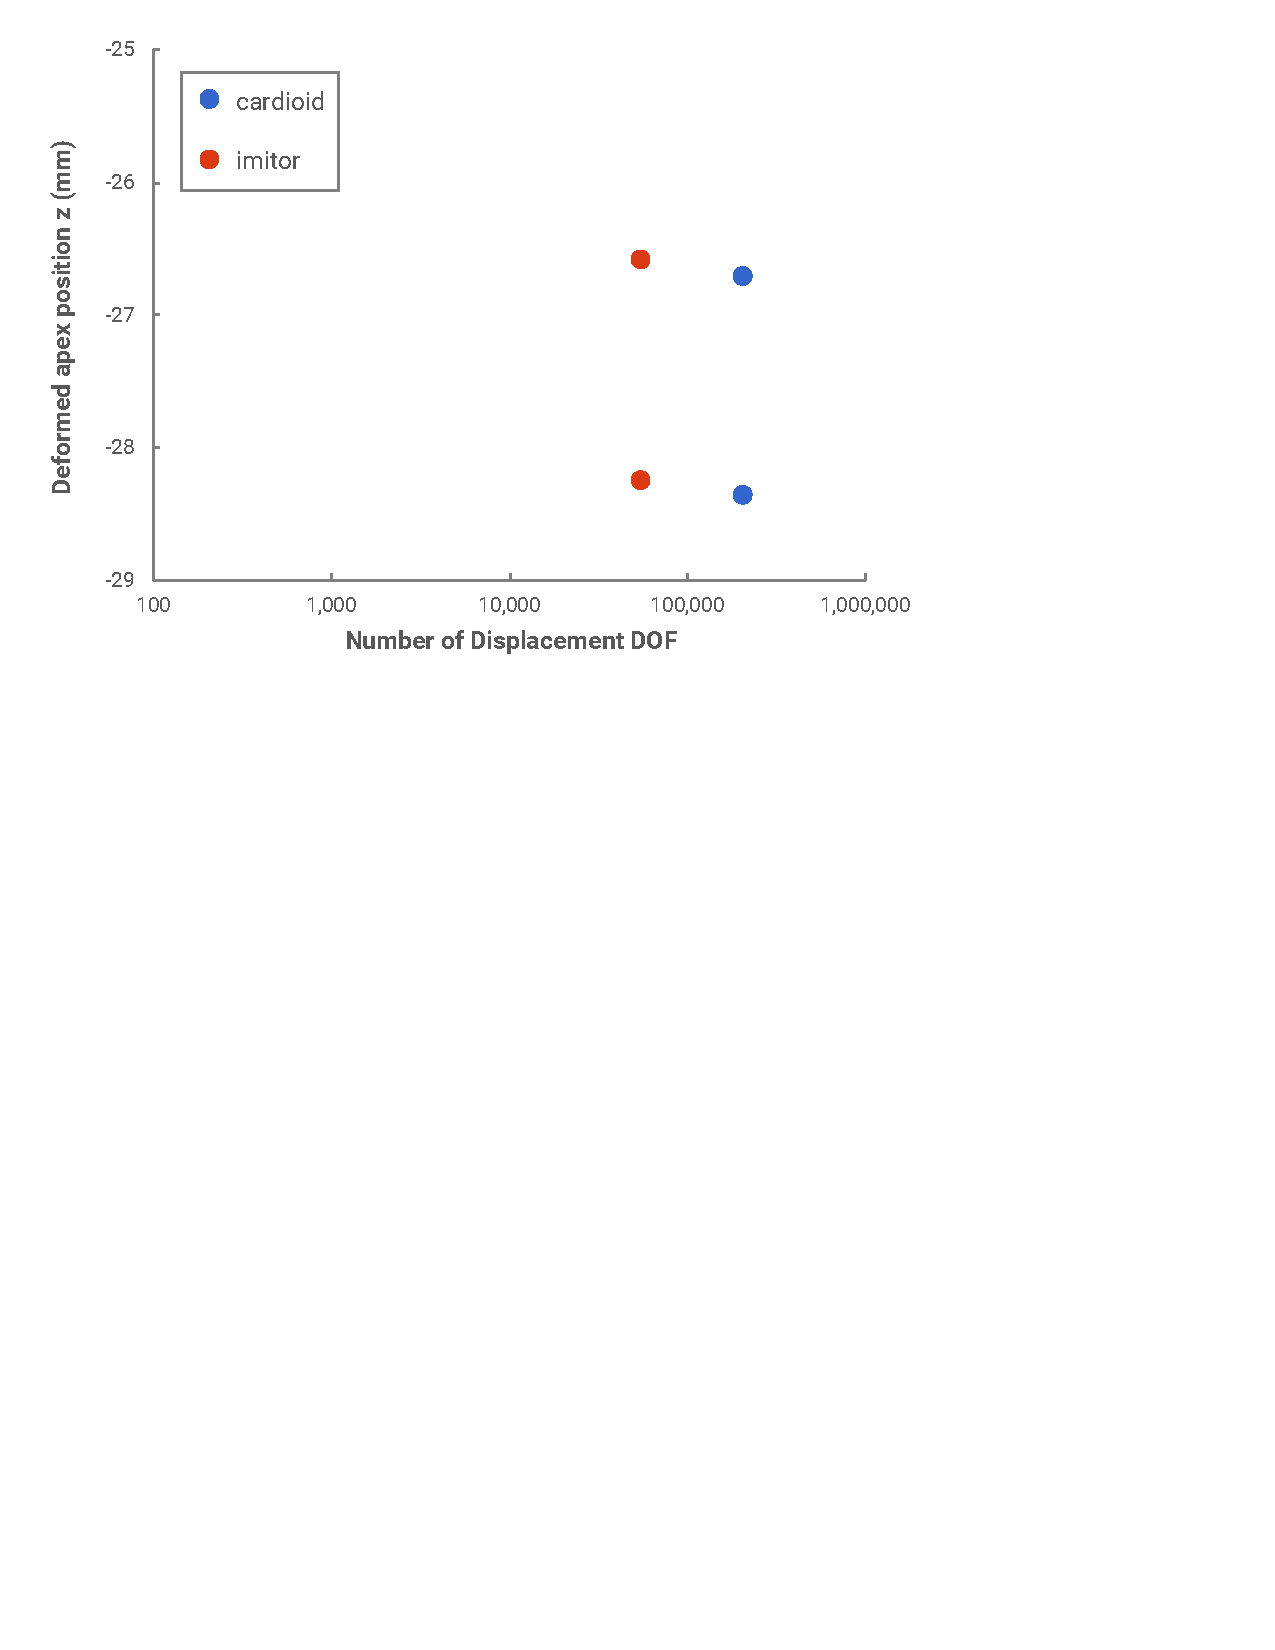
\includegraphics[scale=0.46]{media/5-verif/5-land2/land2-3.pdf}
\label{fig:land2-3}}			
%
\caption{Results for Land P2 verification problem: (a) Deformed position of middle of the ventricle wall, with (b) details at the inflection point (top right) and the apical region (bottom right). Panel (c) shows the deformed position of the apex at the endo- and epicardium for each of the simulation codes.}
\label{fig:land2}
\end{figure}

\begin{figure}[ht!]
\centering
\subfigure[]{%
		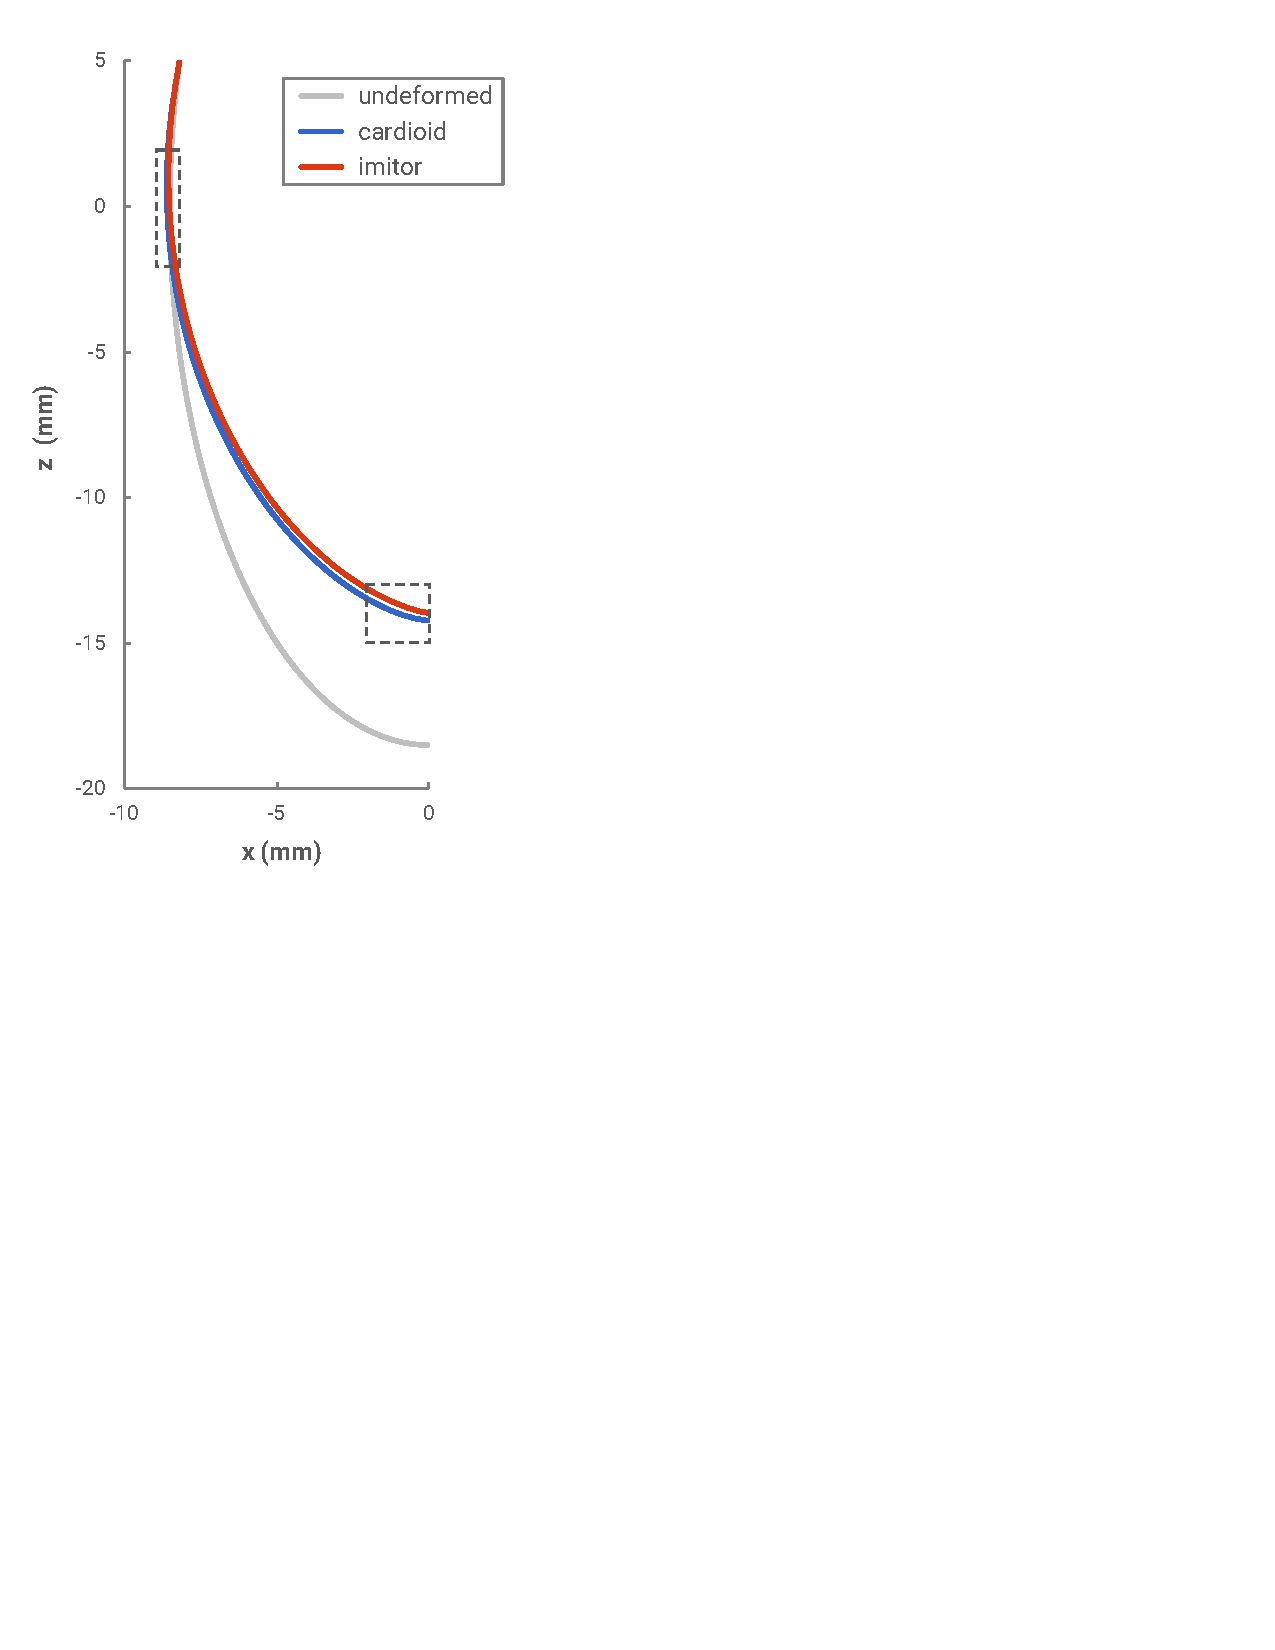
\includegraphics[scale=0.46]{media/5-verif/6-land3/land3-1.pdf}
\label{fig:land3-1}}		
\subfigure[]{%
		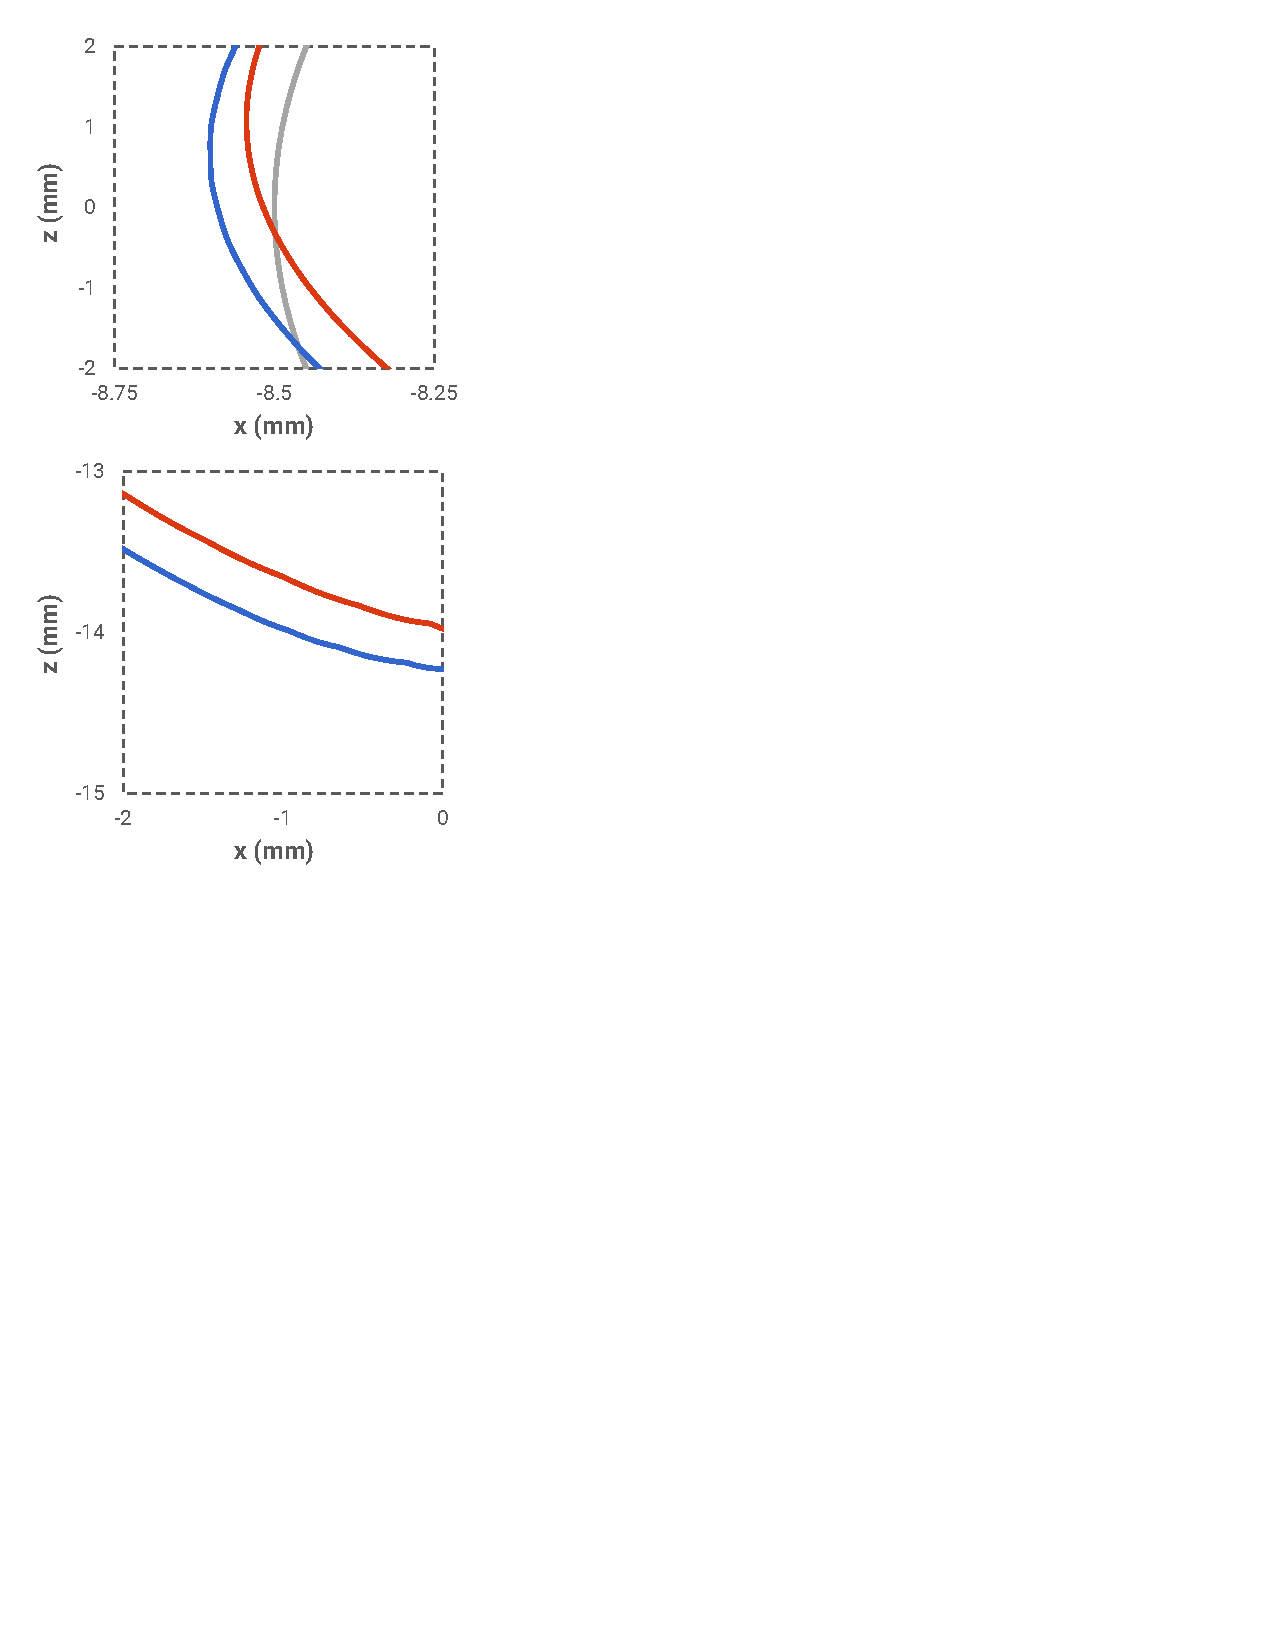
\includegraphics[scale=0.46]{media/5-verif/6-land3/land3-2.pdf}
\label{fig:land3-2}}	
%
\caption{Results for Land P3 verification problem: (a) Deformed position of middle of the ventricle wall, with (b) details at the inflection point (top right) and the apical region (bottom right).}
\label{fig:land3}
\end{figure}

\begin{figure}[ht!]
\centering
\subfigure[]{%
		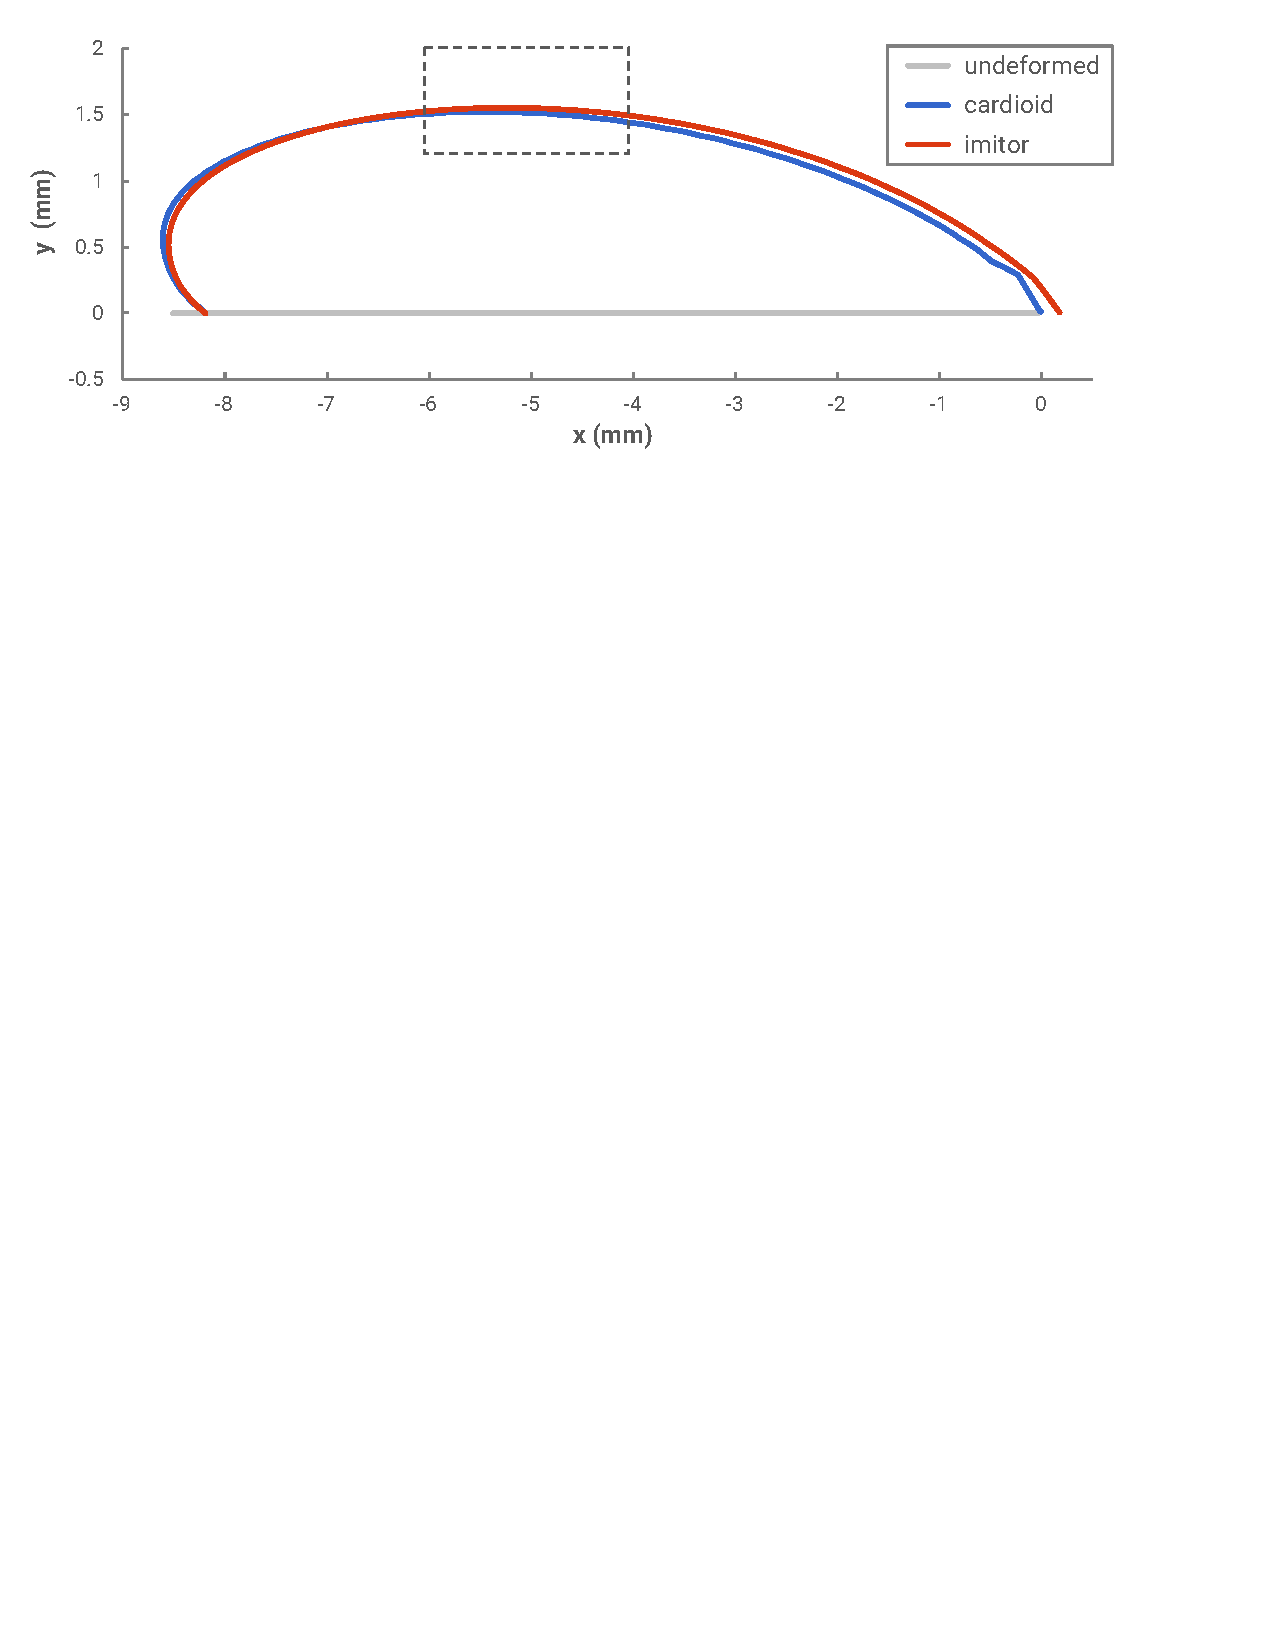
\includegraphics[scale=0.46]{media/5-verif/6-land3/land3-3.pdf}
\label{fig:land3.2-1}}		
\subfigure[]{%
		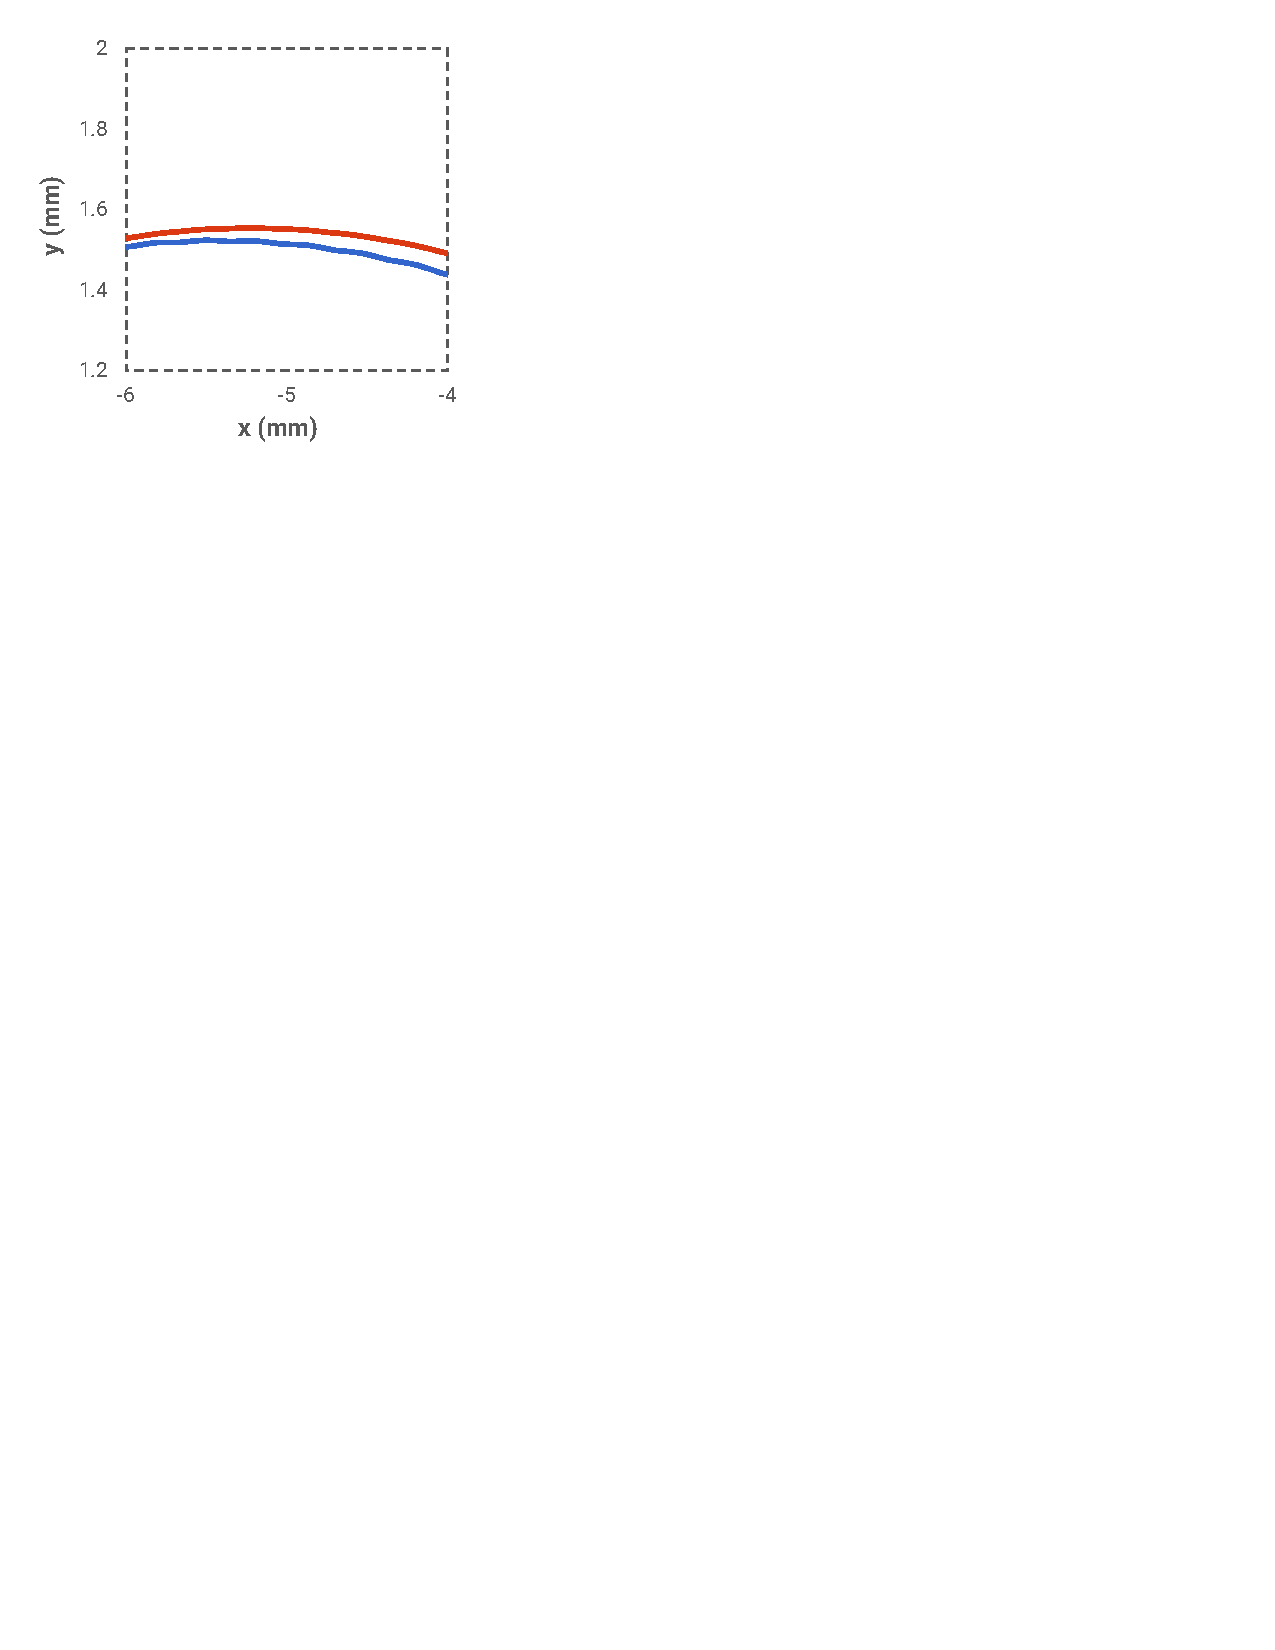
\includegraphics[scale=0.46]{media/5-verif/6-land3/land3-4.pdf}		
\label{fig:land3.2-2}}	
\subfigure[]{%
		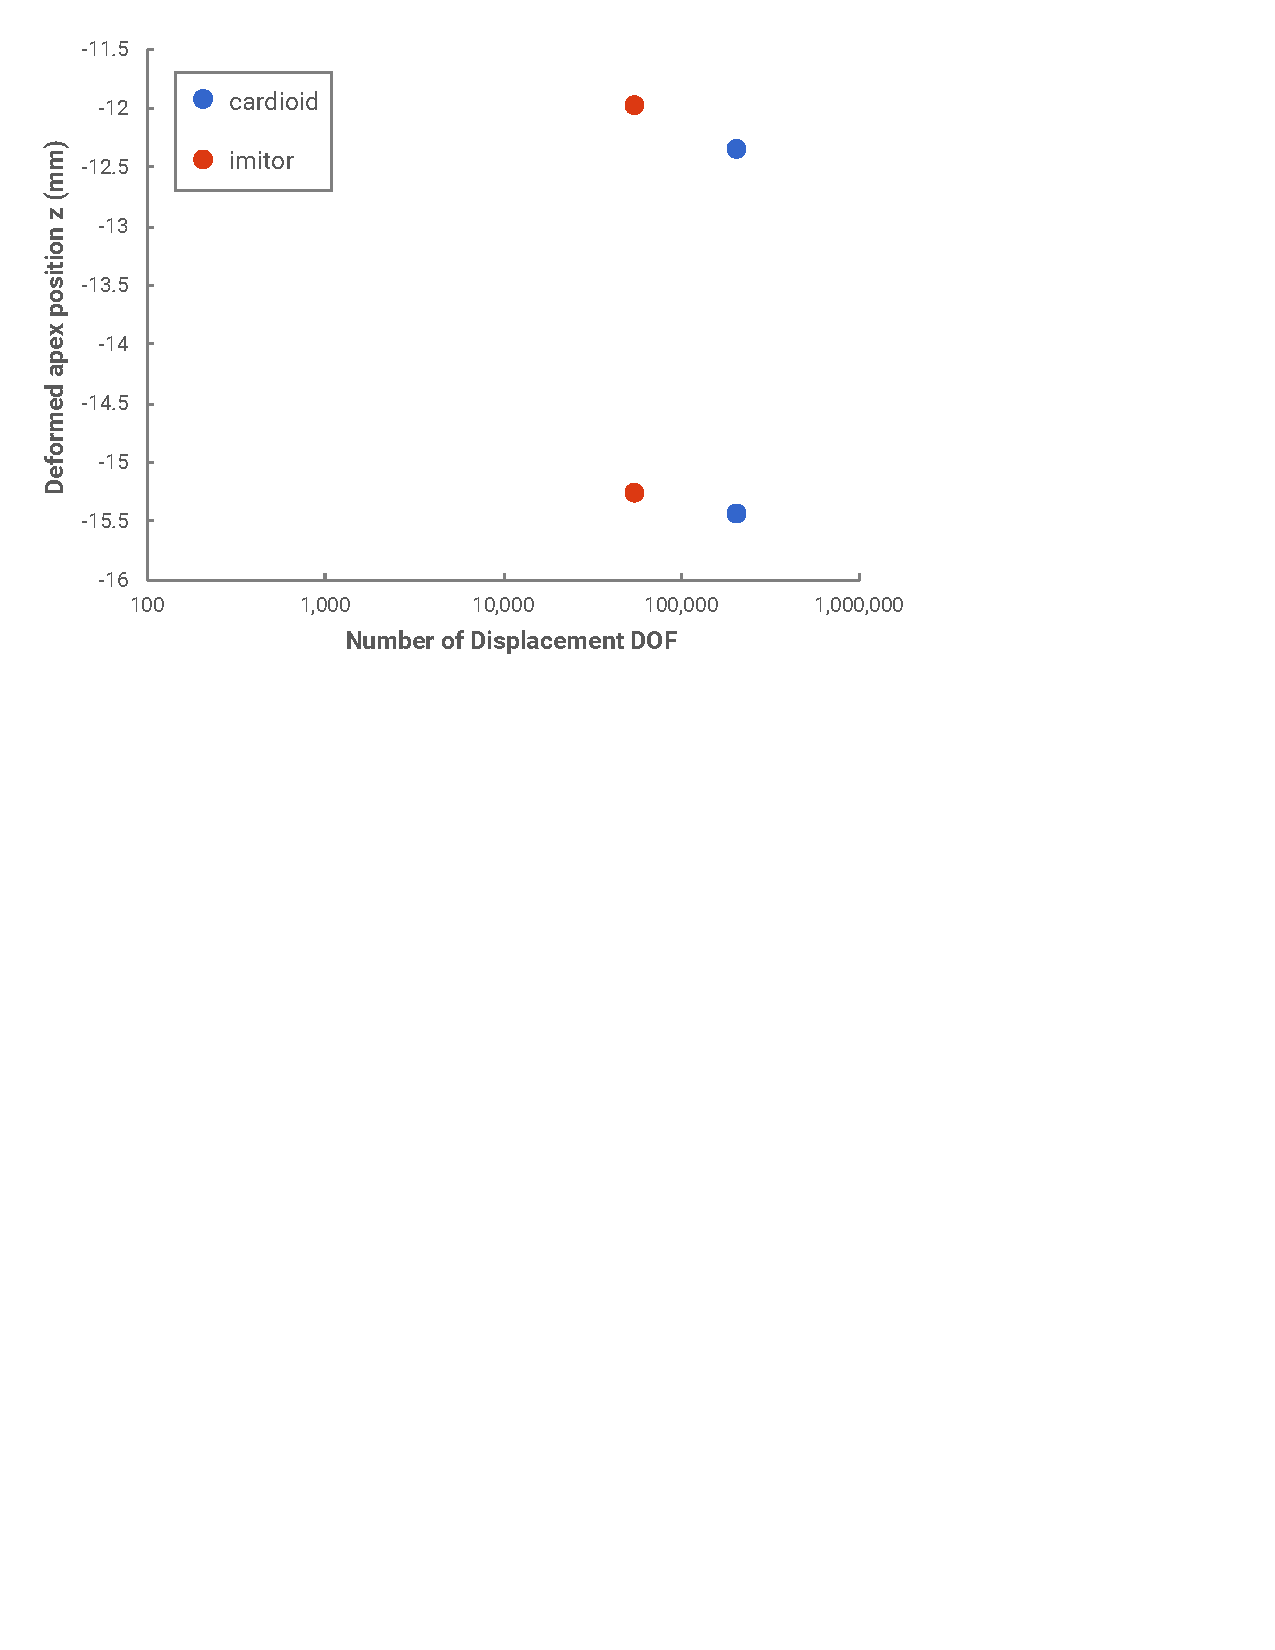
\includegraphics[scale=0.46]{media/5-verif/6-land3/land3-5.pdf}
\label{fig:land3.2-3}}			
	
%
\caption{Results for Land P3 verification problem: (a) The same deformed position of middle of the ventricle wall, shown in the $x-y$ plane, with (b) details at the inflection point. Panel (c) shows the deformed position of the apex at the endo- and epicardium for each of the simulation codes.}
\label{fig:land3.2}
\end{figure}
